\documentclass[12pt,]{krantz}
\usepackage{lmodern}
\usepackage{amssymb,amsmath}
\usepackage{ifxetex,ifluatex}
\usepackage{fixltx2e} % provides \textsubscript
\ifnum 0\ifxetex 1\fi\ifluatex 1\fi=0 % if pdftex
  \usepackage[T1]{fontenc}
  \usepackage[utf8]{inputenc}
\else % if luatex or xelatex
  \ifxetex
    \usepackage{mathspec}
  \else
    \usepackage{fontspec}
  \fi
  \defaultfontfeatures{Ligatures=TeX,Scale=MatchLowercase}
    \setmonofont[Mapping=tex-ansi,Scale=0.7]{Source Code Pro}
\fi
% use upquote if available, for straight quotes in verbatim environments
\IfFileExists{upquote.sty}{\usepackage{upquote}}{}
% use microtype if available
\IfFileExists{microtype.sty}{%
\usepackage{microtype}
\UseMicrotypeSet[protrusion]{basicmath} % disable protrusion for tt fonts
}{}
\usepackage[unicode=true]{hyperref}
\PassOptionsToPackage{usenames,dvipsnames}{color} % color is loaded by hyperref
\hypersetup{
            pdftitle={Introduction to Data Science},
            pdfauthor={Hui Lin and Ming Li},
            colorlinks=true,
            linkcolor=Maroon,
            citecolor=Blue,
            urlcolor=Blue,
            breaklinks=true}
\urlstyle{same}  % don't use monospace font for urls
\usepackage{natbib}
\bibliographystyle{apalike}
\usepackage{color}
\usepackage{fancyvrb}
\newcommand{\VerbBar}{|}
\newcommand{\VERB}{\Verb[commandchars=\\\{\}]}
\DefineVerbatimEnvironment{Highlighting}{Verbatim}{commandchars=\\\{\}}
% Add ',fontsize=\small' for more characters per line
\usepackage{framed}
\definecolor{shadecolor}{RGB}{248,248,248}
\newenvironment{Shaded}{\begin{snugshade}}{\end{snugshade}}
\newcommand{\KeywordTok}[1]{\textcolor[rgb]{0.13,0.29,0.53}{\textbf{{#1}}}}
\newcommand{\DataTypeTok}[1]{\textcolor[rgb]{0.13,0.29,0.53}{{#1}}}
\newcommand{\DecValTok}[1]{\textcolor[rgb]{0.00,0.00,0.81}{{#1}}}
\newcommand{\BaseNTok}[1]{\textcolor[rgb]{0.00,0.00,0.81}{{#1}}}
\newcommand{\FloatTok}[1]{\textcolor[rgb]{0.00,0.00,0.81}{{#1}}}
\newcommand{\ConstantTok}[1]{\textcolor[rgb]{0.00,0.00,0.00}{{#1}}}
\newcommand{\CharTok}[1]{\textcolor[rgb]{0.31,0.60,0.02}{{#1}}}
\newcommand{\SpecialCharTok}[1]{\textcolor[rgb]{0.00,0.00,0.00}{{#1}}}
\newcommand{\StringTok}[1]{\textcolor[rgb]{0.31,0.60,0.02}{{#1}}}
\newcommand{\VerbatimStringTok}[1]{\textcolor[rgb]{0.31,0.60,0.02}{{#1}}}
\newcommand{\SpecialStringTok}[1]{\textcolor[rgb]{0.31,0.60,0.02}{{#1}}}
\newcommand{\ImportTok}[1]{{#1}}
\newcommand{\CommentTok}[1]{\textcolor[rgb]{0.56,0.35,0.01}{\textit{{#1}}}}
\newcommand{\DocumentationTok}[1]{\textcolor[rgb]{0.56,0.35,0.01}{\textbf{\textit{{#1}}}}}
\newcommand{\AnnotationTok}[1]{\textcolor[rgb]{0.56,0.35,0.01}{\textbf{\textit{{#1}}}}}
\newcommand{\CommentVarTok}[1]{\textcolor[rgb]{0.56,0.35,0.01}{\textbf{\textit{{#1}}}}}
\newcommand{\OtherTok}[1]{\textcolor[rgb]{0.56,0.35,0.01}{{#1}}}
\newcommand{\FunctionTok}[1]{\textcolor[rgb]{0.00,0.00,0.00}{{#1}}}
\newcommand{\VariableTok}[1]{\textcolor[rgb]{0.00,0.00,0.00}{{#1}}}
\newcommand{\ControlFlowTok}[1]{\textcolor[rgb]{0.13,0.29,0.53}{\textbf{{#1}}}}
\newcommand{\OperatorTok}[1]{\textcolor[rgb]{0.81,0.36,0.00}{\textbf{{#1}}}}
\newcommand{\BuiltInTok}[1]{{#1}}
\newcommand{\ExtensionTok}[1]{{#1}}
\newcommand{\PreprocessorTok}[1]{\textcolor[rgb]{0.56,0.35,0.01}{\textit{{#1}}}}
\newcommand{\AttributeTok}[1]{\textcolor[rgb]{0.77,0.63,0.00}{{#1}}}
\newcommand{\RegionMarkerTok}[1]{{#1}}
\newcommand{\InformationTok}[1]{\textcolor[rgb]{0.56,0.35,0.01}{\textbf{\textit{{#1}}}}}
\newcommand{\WarningTok}[1]{\textcolor[rgb]{0.56,0.35,0.01}{\textbf{\textit{{#1}}}}}
\newcommand{\AlertTok}[1]{\textcolor[rgb]{0.94,0.16,0.16}{{#1}}}
\newcommand{\ErrorTok}[1]{\textcolor[rgb]{0.64,0.00,0.00}{\textbf{{#1}}}}
\newcommand{\NormalTok}[1]{{#1}}
\usepackage{longtable,booktabs}
\usepackage{graphicx,grffile}
\makeatletter
\def\maxwidth{\ifdim\Gin@nat@width>\linewidth\linewidth\else\Gin@nat@width\fi}
\def\maxheight{\ifdim\Gin@nat@height>\textheight\textheight\else\Gin@nat@height\fi}
\makeatother
% Scale images if necessary, so that they will not overflow the page
% margins by default, and it is still possible to overwrite the defaults
% using explicit options in \includegraphics[width, height, ...]{}
\setkeys{Gin}{width=\maxwidth,height=\maxheight,keepaspectratio}
\IfFileExists{parskip.sty}{%
\usepackage{parskip}
}{% else
\setlength{\parindent}{0pt}
\setlength{\parskip}{6pt plus 2pt minus 1pt}
}
\setlength{\emergencystretch}{3em}  % prevent overfull lines
\providecommand{\tightlist}{%
  \setlength{\itemsep}{0pt}\setlength{\parskip}{0pt}}
\setcounter{secnumdepth}{5}
% Redefines (sub)paragraphs to behave more like sections
\ifx\paragraph\undefined\else
\let\oldparagraph\paragraph
\renewcommand{\paragraph}[1]{\oldparagraph{#1}\mbox{}}
\fi
\ifx\subparagraph\undefined\else
\let\oldsubparagraph\subparagraph
\renewcommand{\subparagraph}[1]{\oldsubparagraph{#1}\mbox{}}
\fi
\usepackage{booktabs}
\usepackage{longtable}
\usepackage[bf,singlelinecheck=off]{caption}

\setmainfont[UprightFeatures={SmallCapsFont=AlegreyaSC-Regular}]{Alegreya}

\usepackage{framed,color}
\definecolor{shadecolor}{RGB}{248,248,248}

\renewcommand{\textfraction}{0.05}
\renewcommand{\topfraction}{0.8}
\renewcommand{\bottomfraction}{0.8}
\renewcommand{\floatpagefraction}{0.75}

\renewenvironment{quote}{\begin{VF}}{\end{VF}}
\let\oldhref\href
\renewcommand{\href}[2]{#2\footnote{\url{#1}}}

\ifxetex
  \usepackage{letltxmacro}
  \setlength{\XeTeXLinkMargin}{1pt}
  \LetLtxMacro\SavedIncludeGraphics\includegraphics
  \def\includegraphics#1#{% #1 catches optional stuff (star/opt. arg.)
    \IncludeGraphicsAux{#1}%
  }%
  \newcommand*{\IncludeGraphicsAux}[2]{%
    \XeTeXLinkBox{%
      \SavedIncludeGraphics#1{#2}%
    }%
  }%
\fi

\makeatletter
\newenvironment{kframe}{%
\medskip{}
\setlength{\fboxsep}{.8em}
 \def\at@end@of@kframe{}%
 \ifinner\ifhmode%
  \def\at@end@of@kframe{\end{minipage}}%
  \begin{minipage}{\columnwidth}%
 \fi\fi%
 \def\FrameCommand##1{\hskip\@totalleftmargin \hskip-\fboxsep
 \colorbox{shadecolor}{##1}\hskip-\fboxsep
     % There is no \\@totalrightmargin, so:
     \hskip-\linewidth \hskip-\@totalleftmargin \hskip\columnwidth}%
 \MakeFramed {\advance\hsize-\width
   \@totalleftmargin\z@ \linewidth\hsize
   \@setminipage}}%
 {\par\unskip\endMakeFramed%
 \at@end@of@kframe}
\makeatother

% \renewenvironment{Shaded}{\begin{kframe}}{\end{kframe}}

\newenvironment{rmdblock}[1]
  {
  \begin{itemize}
  \renewcommand{\labelitemi}{
    \raisebox{-.7\height}[0pt][0pt]{
      {\setkeys{Gin}{width=3em,keepaspectratio}\includegraphics{images/#1}}
    }
  }
  \setlength{\fboxsep}{1em}
  \begin{kframe}
  \item
  }
  {
  \end{kframe}
  \end{itemize}
  }
\newenvironment{rmdnote}
  {\begin{rmdblock}{note}}
  {\end{rmdblock}}
\newenvironment{rmdcaution}
  {\begin{rmdblock}{caution}}
  {\end{rmdblock}}
\newenvironment{rmdimportant}
  {\begin{rmdblock}{important}}
  {\end{rmdblock}}
\newenvironment{rmdtip}
  {\begin{rmdblock}{tip}}
  {\end{rmdblock}}
\newenvironment{rmdwarning}
  {\begin{rmdblock}{warning}}
  {\end{rmdblock}}

\usepackage{makeidx}
\makeindex

\urlstyle{tt}

\usepackage{amsthm}
\makeatletter
\def\thm@space@setup{%
  \thm@preskip=8pt plus 2pt minus 4pt
  \thm@postskip=\thm@preskip
}
\makeatother

\frontmatter

\title{Introduction to Data Science}
\author{Hui Lin and Ming Li}
\date{2017-12-28}

\usepackage{amsthm}
\newtheorem{theorem}{Theorem}[chapter]
\newtheorem{lemma}{Lemma}[chapter]
\theoremstyle{definition}
\newtheorem{definition}{Definition}[chapter]
\newtheorem{corollary}{Corollary}[chapter]
\newtheorem{proposition}{Proposition}[chapter]
\theoremstyle{definition}
\newtheorem{example}{Example}[chapter]
\theoremstyle{remark}
\newtheorem*{remark}{Remark}
\begin{document}
\maketitle

%\cleardoublepage\newpage\thispagestyle{empty}\null
%\cleardoublepage\newpage\thispagestyle{empty}\null
%\cleardoublepage\newpage
\thispagestyle{empty}
\begin{center}
%\includegraphics{images/dedication.pdf}
\end{center}

\setlength{\abovedisplayskip}{-5pt}
\setlength{\abovedisplayshortskip}{-5pt}

{
\hypersetup{linkcolor=black}
\setcounter{tocdepth}{2}
\tableofcontents
}
\listoftables
\listoffigures
\chapter*{Preface}\label{preface}


During the first couple years of our career as data scientists, we were
bewildered by all kinds of data science hype. There is a lack of
definition of many basic terminologies such as ``Big Data'' and ``Data
Science.'' How big is big? If someone ran into you asked what data
science was all about, what would you tell them? What is the difference
between the sexy role ``Data Scientist'' and the traditional ``Data
Analyst''? How suddenly came all kinds of machine algorithms? All those
struck us as confusing and vague as real-world data scientists! But we
always felt that there was something real there. After applying data
science for many years, we explored it more and had a much better idea
about data science. And this book is our endeavor to make data science
to a more legitimate field.

\section*{Goal of the Book}\label{goal-of-the-book}


This is an introductory book to data science with a specific focus on
the application. Data Science is a cross-disciplinary subject involving
hands-on experience and business problem-solving exposures. The majority
of existing introduction books on data science are about the modeling
techniques and the implementation of models using R or Python. However,
they fail to introduce data science in a context of the industrial
environment. Moreover, a crucial part, the art of data science in
practice, is often missing. This book intends to fill the gap.

Some key features of this book are as follows:

\begin{itemize}
\item
  It is comprehensive. It covers not only technical skills but also soft
  skills and big data environment in the industry.
\item
  It is hands-on. We provide the data and repeatable R and Python code.
  You can repeat the analysis in the book using the data and code
  provided. We also suggest you perform the analyses with your data
  whenever possible. You can only learn data science by doing it!
\item
  It is based on context. We put methods in the context of industrial
  data science questions.
\item
  Where appropriate, we point you to more advanced materials on models
  to dive deeper
\end{itemize}

\section*{Who This Book Is For}\label{who-this-book-is-for}


Non-mathematical readers will appreciate the emphasis on problem-solving
with real data across a wide variety of applications and the
reproducibility of the companion R and python code.

Readers should know basic statistical ideas, such as correlation and
linear regression analysis. While the text is biased against complex
equations, a mathematical background is needed for advanced topics.

\section*{What This Book Covers}\label{what-this-book-covers}


Based on industry experience, this book outlines the real world scenario
and points out pitfalls data science practitioners should avoid. It also
covers big data cloud platform and the art of data science such as soft
skills. We use R as the main tool and provide code for both R and
Python.

\section*{Conventions}\label{conventions}


\section*{Acknowledgements}\label{acknowledgements}


\mainmatter

\chapter{Introduction}\label{introduction}

Interest in data science is at an all-time high and has exploded in
popularity in the last couple of years. Data scientists today are from
various backgrounds. If someone ran into you asked what data science was
all about, what would you tell them? It is not easy to answer. Data
science is one of the areas where if you ask ten people you get ten
different answers. It is not well-defined as an academic subject but
broadly used in the industry. Media has been hyping about ``Data
Science'' ``Big Data'' and ``Artificial Intelligence'' over the fast few
years. With the data science hype picking up stream, many professionals
changed their titles to ``Data Scientist'' without any of the necessary
qualifications. Your first reaction to all of this might be some
combination of skepticism and confusion. We want to address this up
front that: we had that exact reaction. To make things clear, let's
start with the fundamental question.

\section{What is data science?}\label{what-is-data-science}

David Donoho \citep{data50} summarizes in ``50 Years of Data Science''
the main recurring ``Memes'' about data sciences:

\begin{enumerate}
\def\labelenumi{\arabic{enumi}.}
\tightlist
\item
  The `Big Data' Meme
\item
  The `Skills' Meme
\item
  The `Jobs' Meme
\end{enumerate}

Everyone should have heard about big data. Data science trainees now
need the skills to cope with such big data sets. What are those skills?
You may hear about: Hadoop, a system using Map/Reduce to process large
data sets distributed across a cluster of computers. The new skills are
for dealing with organizational artifacts of large-scale cluster
computing but not for better solving the real problem. A lot of data on
its own is worthless. It isn't the size of the data that's important.
It's what you do with it. The big data skills that so many are touting
today are not skills for better solving the real problem of inference
from data.

We are transiting to universal connectivity with a deluge of data
filling telecom servers. But these facts don't immediately create a
science. The statisticians and computer scientists have been laying the
groundwork for data science for at least 50 years. Today's data science
is an enlargement and combination of statistics and computer science
rather than a brand new discipline.

Data Science doesn't come out of the blue. Its predecessor is data
analysis. Back in 1962, John Tukey wrote in ``The Future of Data
Analysis'':

\begin{quote}
For a long time I have thought I was a statistician, interested in
inferences from the particular to the general. But as I have watched
mathematical statistics evolve, I have had cause to wonder and to doubt.
\ldots{}All in all, I have come to feel that my central interest is in
data analysis, which I take to include, among other things: procedures
for analyzing data, techniques for interpreting the results of such
procedures, ways of planning the gathering of data to make its analysis
easier, more precise or more accurate, and all the machinery and results
of (mathematical) statistics which apply to analyzing data.
\end{quote}

It deeply shocked his academic readers. Aren't you supposed to present
something mathematically precise, such as definitions, theorems, and
proofs? If we use one sentence to summarize what John said, it is:

\begin{quote}
data analysis is more than mathematics.
\end{quote}

In September 2015, the University of Michigan made plans to invest \$100
million over the next five years in a new Data Science Initiative (DSI)
that will enhance opportunities for student and faculty researchers
across the university to tap into the enormous potential of big data.
How does DSI define Data science? Their website gives us an idea:

\begin{quote}
``This coupling of scientific discovery and practice involves the
collection, management, processing, analysis, visualization, and
interpretation of vast amounts of heterogeneous data associated with a
diverse array of scientific, translational, and interdisciplinary
applications.''
\end{quote}

How about data scientist? Here is a list of somewhat whimsical
definitions for a ``data scientist'':

\begin{itemize}
\tightlist
\item
  ``A data scientist is a data analyst who lives in California''
\item
  ``A data scientist is someone who is better at statistics than any
  software engineer and better at software engineering than any
  statistician.''
\item
  ``A data scientist is a statistician who lives in San Francisco.''
\item
  ``Data Science is statistics on a Mac.''
\end{itemize}

There is lots of confusion between Data Scientist, Statistician,
Business/Financial/Risk(etc.) Analyst and BI professional due to the
apparent intersections among skillsets. We see data science as a
discipline to make sense of data. The techniques and methodologies of
data science stem from the fields of computer science and statistics.
One of the most well-cited diagrams describing the area comes from Drew
Conway where he suggested data science is the intersection of hacking
skills, math and stats knowledge, and substantial expertise. This
diagram might be a bit of an oversimplification, but it's a great start.

There are almost as many definitions of data science as there are data
scientists. Instead of listing some of these definitions, it might be
more informative to let the subject matter define the field.

Let's start from a brief history of data science. If you hit up the
Google Trends website which shows search keyword information over time
and check the term ``data science,'' you will find the history of data
science goes back a little further than 2004. From the way media
describes it, you may feel machine learning algorithms were just
invented last month, and there was never ``big'' data before Google.
That is not true. There are new and exciting developments of data
science, but many of the techniques we are using are based on decades of
work by statisticians, computer scientists, mathematicians and
scientists of all types.

\begin{figure}[htbp]
\centering
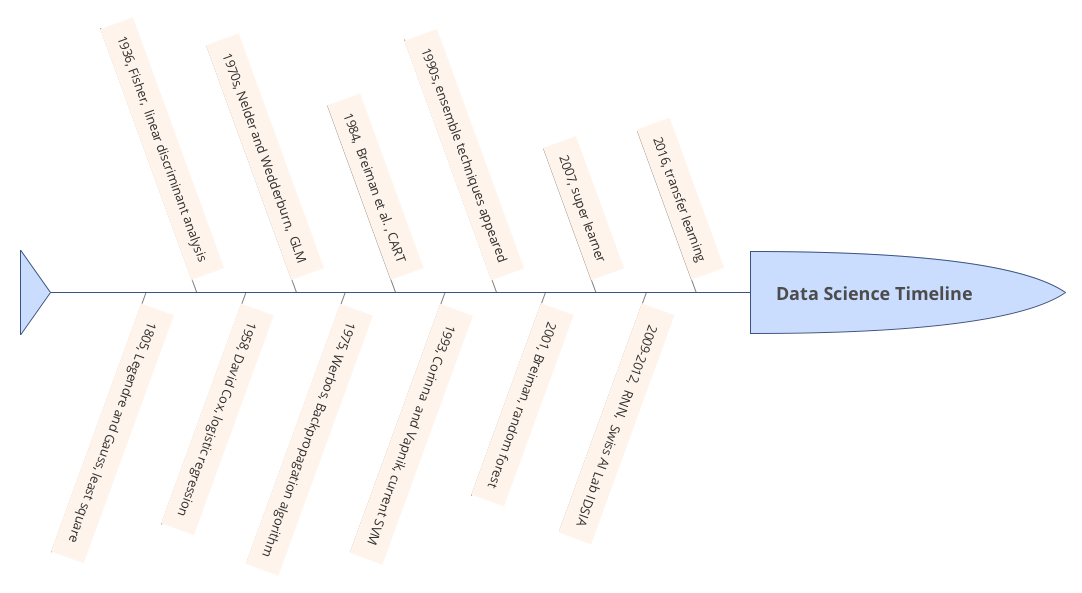
\includegraphics{images/DataScienceTimeline.png}
\caption{Data Science Timeline}
\end{figure}

In the early 19th century when Legendre and Gauss came up the least
squares method for linear regression, only physicists would use it to
fit linear regression. Now, even non-technical people can fit linear
regressions using excel. In 1936 Fisher came up with linear discriminant
analysis. In the 1940s, we had another widely used model -- logistic
regression. In the 1970s, Nelder and Wedderburn formulated ``generalized
linear model (GLM)'' which:

\begin{quote}
``generalized linear regression by allowing the linear model to be
related to the response variable via a link function and by allowing the
magnitude of the variance of each measurement to be a function of its
predicted value.'' {[}from Wikipedia{]}
\end{quote}

By the end of the 1970s, there was a range of analytical models and most
of them were linear because computers were not powerful enough to fit
non-linear model until the 1980s.

In 1984 Breiman et al. introduced classification and regression tree
(CART) which is one of the oldest and most utilized classification and
regression techniques. After that Ross Quinlan came up with more tree
algorithms such as ID3, C4.5, and C5.0. In the 1990s, ensemble
techniques (methods that combine many models' predictions) began to
appear. Bagging is a general approach that uses bootstrapping in
conjunction with any regression or classification model to construct an
ensemble. Based on the ensemble idea, Breiman came up with random forest
in 2001. Later, Yoav Freund and Robert Schapire came up with the
AdaBoost.M1 algorithm. Benefiting from the increasing availability of
digitized information, and the possibility to distribute that via the
internet, the toolbox has been expanding fast. The applications include
business, health, biology, social science, politics, etc.

John Tukey identified four forces driving data analysis (there was no
``data science'' then):

\begin{enumerate}
\def\labelenumi{\arabic{enumi}.}
\tightlist
\item
  The formal theories of math and statistics
\item
  Acceleration of developments in computers and display devices
\item
  The challenge, in many fields, of more and ever larger bodies of data
\item
  The emphasis on quantification in an ever wider variety of disciplines
\end{enumerate}

Tukey's 1962 list is surprisingly modern. Let's inspect those points in
today's context. There is always a time gap between a theory and its
application. We had the theories much earlier than application.
Fortunately, for the past 50 years, statisticians have been laying the
theoretical groundwork for constructing ``data science'' today. The
development of computers enables us to calculate much faster and deliver
results in a friendly and intuitive way. The striking transition to the
internet of things generates vast amounts of commercial data. Industries
have also sensed the value of exploiting that data. Data science seems
certain to be a major preoccupation of commercial life in coming
decades. All the four forces John identified exist today and have been
driving data science.

\section{What kind of questions can data science
solve?}\label{what-kind-of-questions-can-data-science-solve}

\subsection{Prerequisites}\label{prerequisites}

Data science is not a panacea, and data scientists are not magicians.
There are problems data science can't help. It is best to make a
judgment as early in the analytical cycle as possible. Tell your clients
honestly and clearly when you figure data analytics can't give the
answer they want. What kind of questions can data science solve? What
are the requirements for our question?

\begin{enumerate}
\def\labelenumi{\arabic{enumi}.}
\tightlist
\item
  Your question needs to be specific enough
\end{enumerate}

Look at two examples:

\begin{itemize}
\tightlist
\item
  Question 1: How can I increase product sales?
\item
  Question 2: Is the new promotional tool introduced at the beginning of
  this year boosting the annual sales of P1197 in Iowa and Wisconsin?
  (P1197 is an impressive corn seed product from DuPont Pioneer)
\end{itemize}

It is easy to see the difference between the two questions. Question 1
is a grammatically correct question, but it is proper for data analysis
to answer. Why? It is too general. What is the response variable here?
Product sales? Which product? Is it annual sales or monthly sales? What
are the candidate predictors? You nearly can't get any useful
information from the questions. In contrast, question 2 is much more
specific. From the analysis point of view, the response variable is
clearly ``annual sales of P1197 in Iowa and Wisconsin''. Even we don't
know all the predictors, but the variable of interest is ``the new
promotional tool introduced early this year.'' We want to study the
impact of the promotion of the sales. You can start from there and move
on to figure out other variables need to include in the model by further
communication.

As a data scientist, you may start with something general and unspecific
like question 1 and eventually get to question 2. Effective
communication and in-depth domain knowledge about the business problem
are essential to convert a general business question into a solvable
analytical problem. Domain knowledge helps data scientist communicate
with the language the other people can understand and obtain the
required information.

However, defining the question and variables involved don't guarantee
that you can answer it. I have encountered a well-defined supply chain
problem. My client asked about the stock needed for a product in a
particular area. Why can not this question be answered? I did fit a
Multivariate Adaptive Regression Spline (MARS) model and thought I found
a reasonable solution. But it turned out later that the data they gave
me was inaccurate. In some areas, only estimates of past supply figures
were available. The lesson lends itself to the next point.

\begin{enumerate}
\def\labelenumi{\arabic{enumi}.}
\setcounter{enumi}{1}
\tightlist
\item
  You need to have sound and relevant data
\end{enumerate}

One cannot make a silk purse out of a sow's ear. Data scientists need
data, sound and relevant data. The supply problem is a case in point.
There was relevant data, but not sound. All the later analytics based on
that data was a building on sand. Of course, data nearly almost have
noise, but it has to be in a certain range. Generally speaking, the
accuracy requirement for the independent variables of interest and
response variable is higher than others. In question 2, it is data
related to the ``new promotion'' and ``sales of P1197''.

The data has to be helpful for the question. If you want to predict
which product consumers are most likely to buy in the next three months,
you need to have historical purchasing data: the last buying time, the
amount of invoice, coupons and so on. Information about customers'
credit card number, ID number, the email address is not going to help.

Often the quality of the data is more important than the quantity, but
the quantity cannot be overlooked. In the premise of guaranteeing
quality, usually the more data, the better. If you have a specific and
reasonable question, also sound and relevant data, then congratulations,
you can start playing data science!

\subsection{Problem type}\label{problem-type}

Many of the data science books classify the various models from a
technical point of view. Such as supervised vs.~unsupervised models,
linear vs.~nonlinear models, parametric models vs.~non-parametric
models, and so on. Here we will continue on ``problem-oriented'' track.
We first introduce different groups of real problems and then present
which models can be used to answer the corresponding category of
questions.

\begin{figure}[htbp]
\centering
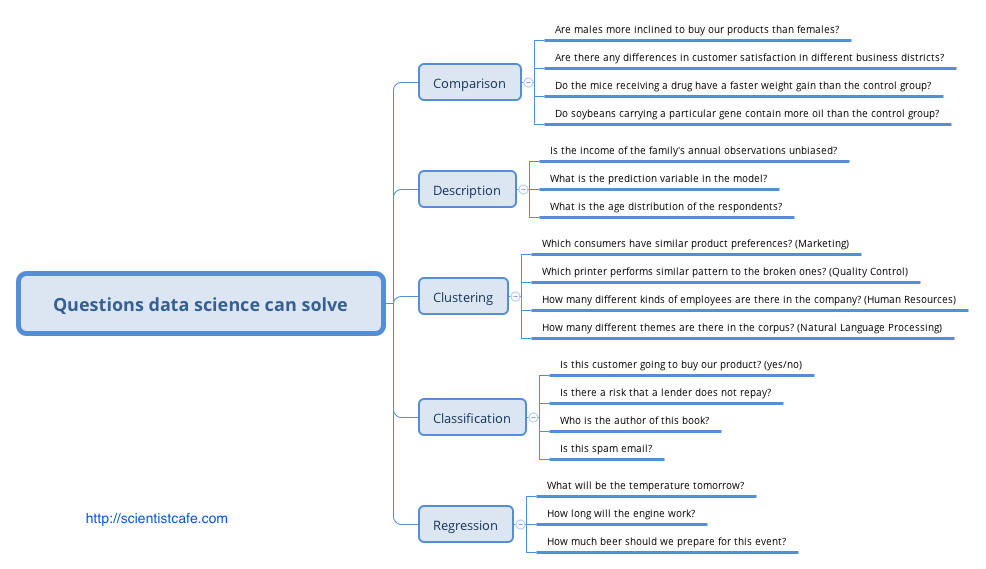
\includegraphics{images/DataScienceQuestion.png}
\caption{Data Science Questions}
\end{figure}

\begin{enumerate}
\def\labelenumi{\arabic{enumi}.}
\tightlist
\item
  Comparison
\end{enumerate}

The first common problem is to compare different groups. Such as: Is A
better in some way than B? Or more comparisons: Is there any difference
among A, B, C in a certain aspect? Here are some examples:

\begin{itemize}
\tightlist
\item
  Are the purchasing amounts different between consumers receiving
  coupons and those without coupons?
\item
  Are males more inclined to buy our products than females?
\item
  Are there any differences in customer satisfaction in different
  business districts?
\item
  Do the mice receiving a drug have a faster weight gain than the
  control group?
\item
  Do soybeans carrying a particular gene contain more oil than the
  control group?
\end{itemize}

For those problems, it is usually to start exploring from the summary
statistics and visualization by groups. After a preliminary
visualization, you can test the differences between treatment and
control group statistically. The commonly used statistical tests are
chi-square test, t-test, and ANOVA. There are also methods using
Bayesian methods. In biology industry, such as new drug development,
crop breeding, mixed effect models are the dominant technique.

\begin{enumerate}
\def\labelenumi{\arabic{enumi}.}
\setcounter{enumi}{1}
\tightlist
\item
  Description
\end{enumerate}

In the problem such as customer segmentation, after you cluster the
sample, the next step is to figure out the profile of each class by
comparing the descriptive statistics of the various variables. Questions
of this kind are:

\begin{itemize}
\tightlist
\item
  Is the income of the family's annual observations unbiased?
\item
  What is the mean/variance of the monthly sales volume of a product in
  different regions?
\item
  What is the difference in the magnitude of the variable? (Decide
  whether the data needs to be standardized)
\item
  What is the prediction variable in the model?
\item
  What is the age distribution of the respondents?
\end{itemize}

Data description is often used to check data, find the appropriate data
preprocessing method, and demonstrate the model results.

\begin{enumerate}
\def\labelenumi{\arabic{enumi}.}
\setcounter{enumi}{2}
\tightlist
\item
  Clustering
\end{enumerate}

Clustering is a widespread problem, which is usually related to
classification. Clustering answers questions like:

\begin{itemize}
\tightlist
\item
  Which consumers have similar product preferences? (Marketing)
\item
  Which printer performs similar pattern to the broken ones? (Quality
  Control)
\item
  How many different kinds of employees are there in the company? (Human
  Resources)
\item
  How many different themes are there in the corpus? (Natural Language
  Processing)
\end{itemize}

Note that clustering is unsupervised learning. The most common
clustering algorithms include K-Means and Hierarchical Clustering.

\begin{enumerate}
\def\labelenumi{\arabic{enumi}.}
\setcounter{enumi}{3}
\tightlist
\item
  Classification
\end{enumerate}

Usually, a labeled sample set is used as a training set to train the
classifier. Then the classifier is used to predict the category of a
future sample. Here are some example questions:

\begin{itemize}
\tightlist
\item
  Is this customer going to buy our product? (yes/no)
\item
  Is there a risk that a lender does not repay?
\item
  Who is the author of this book?
\item
  Is this spam email?
\end{itemize}

There are hundreds of classifiers. In practice, we do not have to try
all the models as long as we fit in several of the best models in most
cases.

\begin{enumerate}
\def\labelenumi{\arabic{enumi}.}
\setcounter{enumi}{4}
\tightlist
\item
  Regression
\end{enumerate}

In general, regression deals with the problem of ``how much is it?'' and
return a numerical answer. In some cases, it is necessary to coerce the
model results to be 0, or round the result to the nearest integer. It is
the most common problem.

\begin{itemize}
\tightlist
\item
  What will be the temperature tomorrow?
\item
  What will be the company's sales in the fourth quarter of this year?
\item
  How long will the engine work?
\item
  How much beer should we prepare for this event?
\end{itemize}

\section{Data Scientist Skill Set}\label{data-scientist-skill-set}

We talked about the bewildering definitions of data scientist. What are
the required skills for a data scientist?

\begin{itemize}
\tightlist
\item
  Educational Background
\end{itemize}

Most of the data scientists today have undergraduate or higher degree
from one of the following areas: computer science, electronic
engineering, mathematics or statistics. According to a 2017 survey, 25\%
of US data scientists have a Ph.D.~degree, 64\% have a Master's degree,
and 11\% are Bachelors.

\begin{itemize}
\tightlist
\item
  Database Skills
\end{itemize}

Data scientists in the industry need to use SQL to pull data from the
database. So it is necessary to be familiar with how data is structured
and how to do basic data manipulation using SQL. Many
statistics/mathematics students do not have experience with SQL in
school. Don't worry. If you are proficient in one programming language,
it is easy to pick up SQL. The main purpose of graduate school should be
to develop the ability to learn and analytical thinking rather than the
technical skills. Even the technical skills are necessary to enter the
professional area. Most of the skills needed at work are not taught in
school.

\begin{itemize}
\tightlist
\item
  Programming Skills
\end{itemize}

Programming skills are critical for data scientists. According to a 2017
survey from
\href{http://www.burtchworks.com/2017/06/19/2017-sas-r-python-flash-survey-results/}{Burtch
Works}, 97\% of the data scientists today using R or Python. We will
provide exemplary code for both in this book. There is not one
``have-to-use'' tool. The goal is to solve the problem not which tool to
choose. However, a good tool needs to be flexible and scalable.

\begin{itemize}
\tightlist
\item
  Modeling Skills
\end{itemize}

Data scientists need to know statistical and machine learning models.
There is no clear line separating these two. Many statistical models are
also machine learning models, vice versa. Generally speaking, a data
scientist is familiar with basic statistical tests such as t-test,
chi-square test, and analysis of variance. They can explain the
difference between Spearman rank correlation and Pearson correlation, be
aware of basic sampling schemes, such as Simple Random Sampling,
Stratified Random Sampling, and Multi-Stage Sampling. Know commonly used
probability distributions such as Normal distribution, Binomial
distribution, Poisson distribution, F distribution, T distribution, and
Chi-square distribution. Experimental design plays a significant role in
the biological study. Understanding the main tenants of Bayesian methods
is necessary (at least be able to write the Bayes theorem on the
whiteboard and know what does it mean). Know the difference between
supervised and unsupervised learning. Understand commonly used cluster
algorithms, classifiers, and regression models. Some powerful tools in
predictive analytics are tree models (such as random forest and
AdaBoost) and penalized model (such as lasso and SVM). Data scientist
working on social science (such as consumer awareness surveys), also
needs to know the latent variable model, such as exploratory factor
analysis, confirmatory factor analysis, structural equation model.

Is the list getting a little scary? It can get even longer. Don't worry
if you don't know all of them now. You will learn as you go. Standard
mathematics, statistics or computer science training in graduate school
can get you started. But you have to learn lots of new skills after
school. Learning is happening increasingly outside of formal educational
settings and in unsupervised environments. An excellent data scientist
must be a lifetime learner. Fortunately, technological advantages
provide new tools and opportunities for lifetime learners, MOOC, online
data science workshops and various online tutorials. So above all, being
a \textbf{life-time learner} is the most critical.

\begin{itemize}
\tightlist
\item
  Soft Skills
\end{itemize}

In addition to technical knowledge, there are some critical soft skills.
These include the ability to translate practical problems into data
problems, excellent communication skill, attention to detail,
storytelling and so on. We will discuss it in a later chapter in more
detail.

\begin{figure}[htbp]
\centering
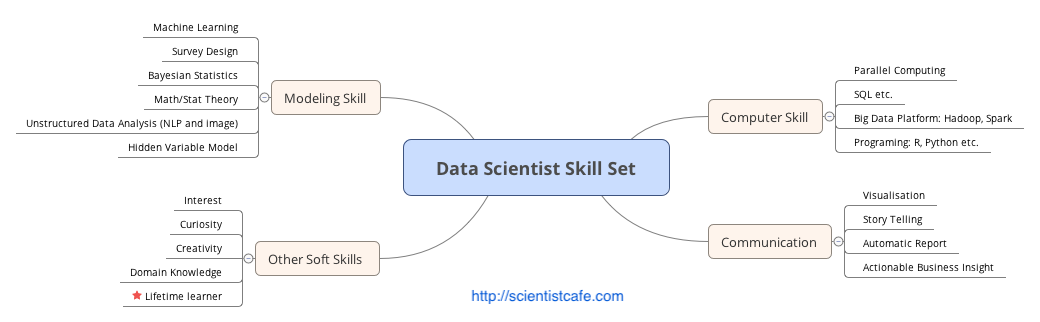
\includegraphics{images/SkillEN.png}
\caption{Data Scientist Skill Set}
\end{figure}

\section{Types of Learning}\label{types-of-learning}

There are three broad groups of styles: supervised learning,
reinforcement learning, and unsupervised learning.

In supervised learning, each observation of the predictor measurement(s)
corresponds to a response measurement. There are two flavors of
supervised learning: regression and classification. In regression, the
response is a real number such as the total net sales in 2017, or the
yield of corn next year. The goal is to approximate the response
measurement as much as possible. In classification, the response is a
class label, such as dichotomous response such as yes/no. The response
can also have more than two categories, such as four segments of
customers. A supervised learning model is a function that maps some
input variables with corresponding parameters to a response y. Modeling
tuning is to adjust the value of parameters to make the mapping fit the
given response. In other words, it is to minimize the discrepancy
between given response and the model output. When the response y is a
real value, it is intuitive to define discrepancy as the squared
difference between model output and given the response. When y is
categorical, there are other ways to measure the difference, such as AUC
or information gain.

In reinforcement learning, the correct input/output pairs are not
present. The model will learn from a sequence of actions and select the
action maximizing the expected sum of the future rewards. There is a
discount factor that makes future rewards less valuable than current
rewards. Reinforcement learning is difficult for the following reasons:

\begin{enumerate}
\def\labelenumi{(\arabic{enumi})}
\item
  The rewards are not instant. If the action sequence is long, it is
  hard to know which action was wrong.
\item
  The rewards are occasional. Each reward does not supply much
  information, so its impact of parameter change is limited. Typically,
  it is not likely to learn a large number of parameters using
  reinforcement learning. However, it is possible for supervised and
  unsupervised learning. The number of parameters in reinforcement
  learning usually range from dozens to maybe 1,000, but not millions.
\end{enumerate}

In unsupervised learning, there is no response variable. For a long
time, the machine learning community overlooked unsupervised learning
except for one called clustering. Moreover, many researchers thought
that clustering was the only form of unsupervised learning. One reason
is that it is hard to define the goal of unsupervised learning
explicitly. Unsupervised learning can be used to do the following:

\begin{enumerate}
\def\labelenumi{(\arabic{enumi})}
\item
  Identify a good internal representation or pattern of the input that
  is useful for subsequent supervised or reinforcement learning, such as
  finding clusters.
\item
  It is a dimension reduction tool that is to provide compact, low
  dimensional representations of the input, such as factor analysis.
\item
  Provide a reduced number of uncorrelated learned features from
  original variables, such as principal component regression.
\end{enumerate}

\begin{figure}[htbp]
\centering
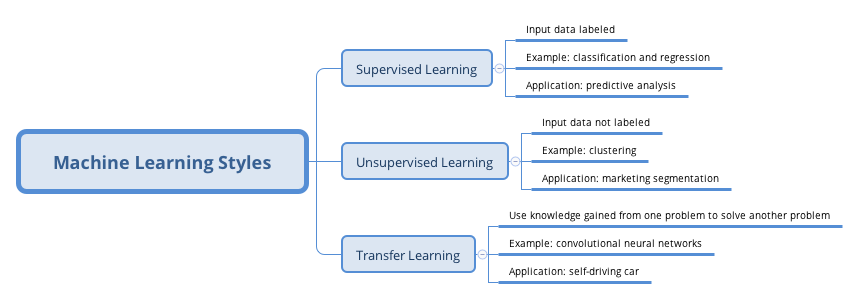
\includegraphics{images/LearningStyles.png}
\caption{Machine Learning Styles}
\end{figure}

\section{Types of Algorithm}\label{types-of-algorithm}

The categorization here is based on the structure (such as tree model,
Regularization Methods) or type of question to answer (such as
regression).\footnote{The summary of various algorithms for data science
  in this section is based on Jason Brownlee's blog ``(A Tour of Machine
  Learning
  Algorithms){[}\url{http://machinelearningmastery.com/a-tour-of-machine-learning-algorithms/}{]}.''
  We added and subtracted some algorithms in each category and gave
  additional comments.} It is far less than perfect but will help to
show a bigger map of different algorithms. Some can be legitimately
classified into multiple categories, such as support vector machine
(SVM) can be a classifier, and can also be used for regression. So you
may see other ways of grouping. Also, the following summary does not
list all the existing algorithms (there are just too many).

\begin{enumerate}
\def\labelenumi{\arabic{enumi}.}
\tightlist
\item
  Regression
\end{enumerate}

Regression can refer to the algorithm or a particular type of problem.
It is supervised learning. Regression is one of the oldest and most
widely used statistical models. It is often called the statistical
machine learning method. Standard regression models are:

\begin{itemize}
\tightlist
\item
  Ordinary Least Squares Regression
\item
  Logistic Regression
\item
  Multivariate Adaptive Regression Splines (MARS)
\item
  Locally Estimated Scatterplot Smoothing (LOESS)
\end{itemize}

The least squares regression and logistic regression are traditional
statistical models. Both of them are highly interpretable. MARS is
similar to neural networks and partial least squares (PLS) in the
respect that they all use surrogate features instead of original
predictors.

They differ in how to create the surrogate features. PLS and neural
networks use linear combinations of the original predictors as surrogate
features \footnote{To be clear on neural networks, the linear
  combinations of predictors are put through non-linear activation
  functions, deeper neural networks have many layers of non-linear
  transformation}. MARS creates two contrasted versions of a predictor
by a truncation point. And LOESS is a non-parametric model, usually only
used in visualization.

\begin{enumerate}
\def\labelenumi{\arabic{enumi}.}
\setcounter{enumi}{1}
\tightlist
\item
  Similarity-based Algorithms
\end{enumerate}

This type of model is based on a similarity measure. There are three
main steps: (1) compare the new sample with the existing ones; (2)
search for the closest sample; (3) and let the response of the nearest
sample be used as the prediction.

\begin{itemize}
\tightlist
\item
  K-Nearest Neighbour {[}KNN{]}
\item
  Learning Vector Quantization {[}LVQ{]}
\item
  Self-Organizing Map {[}SOM{]}
\end{itemize}

The biggest advantage of this type of model is that they are intuitive.
K-Nearest Neighbour is generally the most popular algorithm in this set.
The other two are less common. The key to similarity-based algorithms is
to find an appropriate distance metric for your data.

\begin{enumerate}
\def\labelenumi{\arabic{enumi}.}
\setcounter{enumi}{2}
\tightlist
\item
  Feature Selection Algorithms
\end{enumerate}

The primary purpose of feature selection is to exclude non-information
or redundant variables and also reduce dimension. Although it is
possible that all the independent variables are significant for
explaining the response. But more often, the response is only related to
a portion of the predictors. We will expand the feature selection in
detail later.

\begin{itemize}
\tightlist
\item
  Filter method
\item
  Wrapper method
\item
  Embedded method
\end{itemize}

Filter method focuses on the relationship between a single feature and a
target variable. It evaluates each feature (or an independent variable)
before modeling and selects ``important'' variables.

Wrapper method removes the variable according to particular law and
finds the feature combination that optimizes the model fitting by
evaluating a set of feature combinations. In essence, it is a searching
algorithm.

Embedding method is part of the machine learning model. Some model has
built-in variable selection function such as lasso, and decision tree.

\begin{enumerate}
\def\labelenumi{\arabic{enumi}.}
\setcounter{enumi}{3}
\tightlist
\item
  Regularization Method
\end{enumerate}

This method itself is not a complete model, but rather an add-on to
other models (such as regression models). It appends a penalty function
on the criteria used by the original model to estimate the variables
(such as likelihood function or the sum of squared error). In this way,
it penalizes model complexity and contracts the model parameters. That
is why people call them ``shrinkage method.'' This approach is
advantageous in practice.

\begin{itemize}
\tightlist
\item
  Ridge Regression
\item
  Least Absolute Shrinkage and Selection Operator (LASSO)
\item
  Elastic Net
\end{itemize}

\begin{enumerate}
\def\labelenumi{\arabic{enumi}.}
\setcounter{enumi}{4}
\tightlist
\item
  Decision Tree
\end{enumerate}

Decision trees are no doubt one of the most popular machine learning
algorithms. Thanks to all kinds of software, implementation is a
no-brainer which requires nearly zero understanding of the mechanism.
The followings are some of the common trees:

\begin{itemize}
\tightlist
\item
  Classification and Regression Tree (CART)
\item
  Iterative Dichotomiser 3 (ID3)
\item
  C4.5
\item
  Random Forest
\item
  Gradient Boosting Machines (GBM)
\end{itemize}

\begin{enumerate}
\def\labelenumi{\arabic{enumi}.}
\setcounter{enumi}{5}
\tightlist
\item
  Bayesian Models
\end{enumerate}

People usually confuse Bayes theorem with Bayesian models. Bayes theorem
is an implication of probability theory which gives Bayesian data
analysis its name.

\[Pr(\theta|y)=\frac{Pr(y|\theta)Pr(\theta)}{Pr(y)}\]

The actual Bayesian model is not identical to Bayes theorem. Given a
likelihood, parameters to estimate, and a prior for each parameter, a
Bayesian model treats the estimates as a purely logical consequence of
those assumptions. The resulting estimates are the posterior
distribution which is the relative plausibility of different parameter
values, conditional on the observations. The Bayesian model here is not
strictly in the sense of Bayesian but rather model using Bayes theorem.

\begin{itemize}
\tightlist
\item
  Naïve Bayes
\item
  Averaged One-Dependence Estimators (AODE)
\item
  Bayesian Belief Network (BBN)
\end{itemize}

\begin{enumerate}
\def\labelenumi{\arabic{enumi}.}
\setcounter{enumi}{6}
\tightlist
\item
  Kernel Methods
\end{enumerate}

The most common kernel method is the support vector machine (SVM). This
type of algorithm maps the input data to a higher order vector space
where classification or regression problems are easier to solve.

\begin{itemize}
\tightlist
\item
  Support Vector Machine (SVM)
\item
  Radial Basis Function (RBF)
\item
  Linear Discriminate Analysis (LDA)
\end{itemize}

\begin{enumerate}
\def\labelenumi{\arabic{enumi}.}
\setcounter{enumi}{7}
\tightlist
\item
  Clustering Methods
\end{enumerate}

Like regression, when people mention clustering, sometimes they mean a
class of problems, sometimes a class of algorithms. The clustering
algorithm usually clusters similar samples to categories in a centroidal
or hierarchical manner. The two are the most common clustering methods:

\begin{itemize}
\tightlist
\item
  K-Means
\item
  Hierarchical Clustering
\end{itemize}

\begin{enumerate}
\def\labelenumi{\arabic{enumi}.}
\setcounter{enumi}{8}
\tightlist
\item
  Association Rule
\end{enumerate}

The basic idea of an association rule is: when events occur together
more often than one would expect from their rates of occurrence, such
co-occurrence is an interesting pattern. The most used algorithms are:

\begin{itemize}
\tightlist
\item
  Apriori algorithm
\item
  Eclat algorithm
\end{itemize}

\begin{enumerate}
\def\labelenumi{\arabic{enumi}.}
\setcounter{enumi}{9}
\tightlist
\item
  Artificial Neural Network
\end{enumerate}

The term neural network has evolved to encompass a repertoire of models
and learning methods. There has been lots of hype around the model
family making them seem magical and mysterious. A neural network is a
two-stage regression or classification model. The basic idea is that it
uses linear combinations of the original predictors as surrogate
features, and then the new features are put through non-linear
activation functions to get hidden units in the 2nd stage. When there
are multiple hidden layers, it is called deep learning, another over
hyped term. Among varieties of neural network models, the most widely
used ``vanilla'' net is the single hidden layer back-propagation
network.

\begin{itemize}
\tightlist
\item
  Perceptron Neural Network
\item
  Back Propagation
\item
  Hopield Network
\item
  Self-Organizing Map (SOM)
\item
  Learning Vector Quantization (LVQ)
\end{itemize}

\begin{enumerate}
\def\labelenumi{\arabic{enumi}.}
\setcounter{enumi}{10}
\tightlist
\item
  Deep Learning
\end{enumerate}

The name is a little misleading. As mentioned before, it is multilayer
neural network. It is hyped tremendously especially after AlphaGO
defeated Li Shishi at the board game Go. We don't have too much
experience with the application of deep learning and are not in the
right position to talk more about it. Here are some of the common
algorithms:

\begin{itemize}
\tightlist
\item
  Restricted Boltzmann Machine (RBN)
\item
  Deep Belief Networks (DBN)
\item
  Convolutional Network
\item
  Stacked Autoencoders
\item
  Long short-term memory (LSTM)
\end{itemize}

\begin{enumerate}
\def\labelenumi{\arabic{enumi}.}
\setcounter{enumi}{11}
\tightlist
\item
  Dimensionality Reduction
\end{enumerate}

Its purpose is to construct new features that have significant physical
or statistical characteristics, such as capturing as much of the
variance as possible.

\begin{itemize}
\tightlist
\item
  Principle Component Analysis (PCA)
\item
  Partial Least Square Regression (PLS)
\item
  Multi-Dimensional Scaling (MDS)
\item
  Exploratory Factor Analysis (EFA)
\end{itemize}

PCA attempts to find uncorrelated linear combinations of original
variables that can explain the variance to the greatest extent possible.
EFA also tries to explain as much variance as possible in a lower
dimension. MDS maps the observed similarity to a low dimension, such as
a two-dimensional plane. Instead of extracting underlying components or
latent factors, MDS attempts to find a lower-dimensional map that best
preserves all the observed similarities between items. So it needs to
define a similarity measure as in clustering methods.

\begin{enumerate}
\def\labelenumi{\arabic{enumi}.}
\setcounter{enumi}{12}
\tightlist
\item
  Ensemble Methods
\end{enumerate}

Ensemble method made its debut in the 1990s. The idea is to build a
prediction model by combining the strengths of a collection of simpler
base models. Bagging, originally proposed by Leo Breiman, is one of the
earliest ensemble methods. After that, people developed Random Forest
\citep{Ho1998, amit1997} and Boosting method
\citep{Valiant1984, KV1989}. This is a class of powerful and effective
algorithms.

\begin{itemize}
\tightlist
\item
  Bootstrapped Aggregation (Bagging)
\item
  Random Forest
\item
  Gradient Boosting Machine (GBM)
\end{itemize}

\begin{figure}[htbp]
\centering
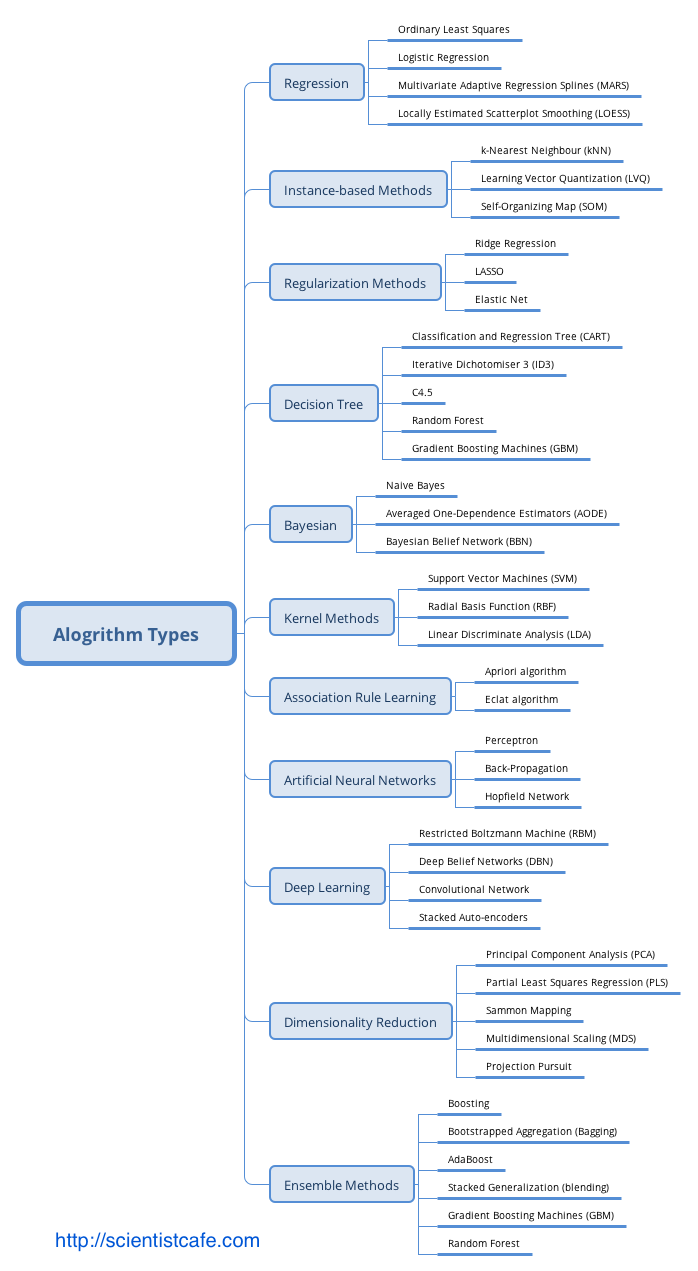
\includegraphics{images/AlogrithmTypes.png}
\caption{Machines Learning Algorithms}
\end{figure}

\chapter{Soft Skills for Data
Scientists}\label{soft-skills-for-data-scientists}

\section{Comparison between Statistician and Data
Scientist}\label{comparison-between-statistician-and-data-scientist}

Statistics as a scientific area can be traced back to 1749 and
statistician as a career has been around for hundreds of years with
well-established theory and application. Data Scientist becomes an
attractive career for only a few years along with the fact that data
size and variety beyond the traditional statistician's toolbox and the
fast-growing of computation power. Statistician and data scientist have
a lot of common backgrounds, but there are also some significant
differences.

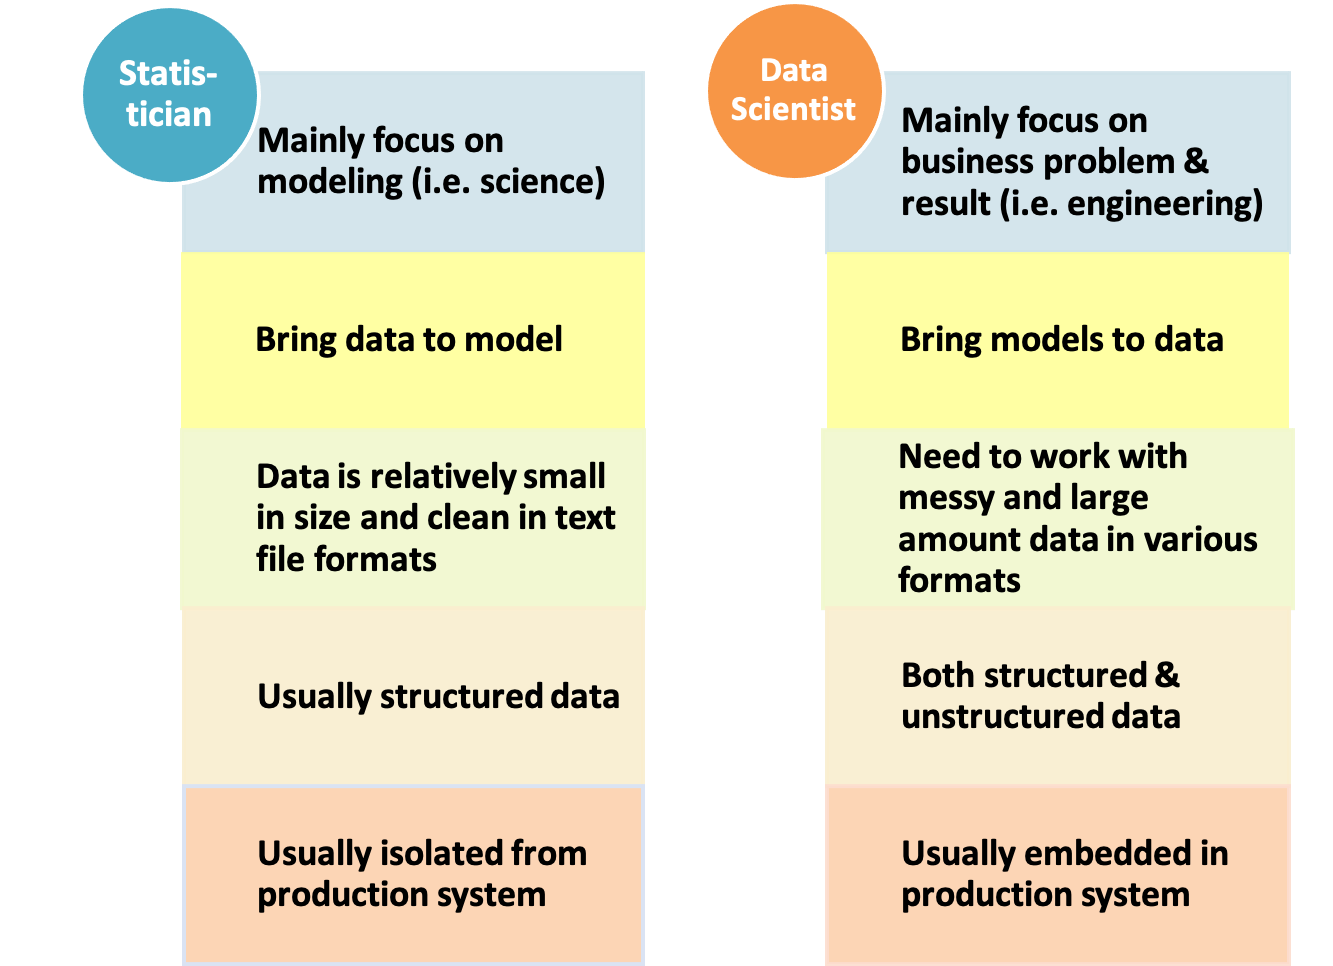
\includegraphics{images/softskill1.png}

Both statistician and data scientist work closely with data. For the
traditional statistician, the data is usually well-formatted text files
with numbers and labels. The size of the data usually can be fitted in a
PC's memory. Comparing to statisticians, data scientists need to deal
with more varieties of data: well-formatted data stored in a database
system with size much larger than a PC's memory or hard-disk; huge
amount of verbatim text, voice, image, and video; real-time streaming
data and other types of records. One particular power of statistics is
that statistician can fit model and make an inference based on limited
data. It is quite common that once the data is given and cleaned, the
majority of the work is developed different models around the data.
Today, data is relatively abundant, and modeling is just part of the
overall effort. The focus is to deliver actionable results. Different
from statisticians, data scientists, sometimes need to fit model on the
cloud instead of reading data in since the data size is too large. From
the entire problem-solving cycle, statisticians are usually not well
integrated with the production system where data is obtained in real
time; while data scientists are more embedded in the production system
and closer to the data generation procedures.

\section{Where Data Science Team
Fits?}\label{where-data-science-team-fits}

During the past decade, a huge amount of data has become available and
readily accessible for analysis in many companies across different
business sectors. The size, complexity, and speed of increment of data
suddenly beyond the traditional scope of statistical analysis or BI
reporting as mentioned above. To leverage the big data, many companies
have established new data science organizations. Companies have gone
through different paths to create their data science and machine
learning organizations. There are three major formats of data science
teams:

\begin{enumerate}
\def\labelenumi{(\arabic{enumi})}
\tightlist
\item
  independent of any current organizations and the team report directly
  to senior leadership;\\
\item
  within each business unit and the team report to business unit
  leaders;\\
\item
  within in the traditional IT organizations and the team report to IT
  leaders.
\end{enumerate}

Companies are different in many aspects, but in general, the most
efficient option to mine big data is a team of data scientist
independent of business units and IT organizations. The independence
enables the data science team to collaborate across business units and
IT organizations more efficiently and the independence also provides
flexibility and potential to solve corporate level strategic big data
problems. For each business units, there are many business unit specific
data science related problems and embedding data scientist within each
business units is also an efficient way to solve business unit specific
data science problems. The full cycle of data science projects from data
to decision (i.e.~Data -\textgreater{} Information -\textgreater{}
Knowledge -\textgreater{} Insight -\textgreater{} Decision) is
relatively difficult to achieve if the data science team is part of
traditional IT organizations.

\section{Beyond Data and Analytics}\label{beyond-data-and-analytics}

Data scientists usually have a good sense of data and analytics, but
data scientist project is more than just data and analytics. A data
science project may involve people with many different roles:

\begin{itemize}
\tightlist
\item
  a business owner or leader to identify opportunities in business
  value; program managers to ensure each data science project fit into
  the overall technical program development;
\item
  data owners and computation resource and infrastructure owners from IT
  department;
\item
  dedicated team to make sure the data and model are under model
  governance and privacy guidelines;
\item
  a team to implement, maintain and refresh the model;
\item
  project managers to coordinate all parties to set periodical tasks so
  that the project meets the preset milestones and delivery results;
\item
  multiple rounds of discussion of resource allocation (i.e.~who will
  pay for the data science project).
\end{itemize}

Effective communication and in-depth domain knowledge about the business
problem are essential requirements for a successful data scientist. A
data scientist will interact with people at various levels ranging from
senior leaders who are setting the corporate strategies to front-line
employees who are doing the daily work. A data scientist needs to have
the capability to view the problem from 10,000 feet above ground, as
well as down to the detail to the very bottom. To convert a business
question into a data problem, a data scientist needs to communicate
using the language the other people can understand and obtain the
required information.

\section{Data Scientist as a Leader}\label{data-scientist-as-a-leader}

During the entire process of data science project defining, planning,
executing and implementation, the data scientist lead needs to be
involved in every step to ensure the business problem is defined
correctly and the business value and success metric are evaluated
reasonably. Corporates are investing heavily in data science and machine
learning with a very high expectation of big return. There are too many
opportunities to introduce unrealistic goal and business impact for a
particular data science project. The leading data scientist need to be
the leader in these discussions to define the goal backed by data and
analytics. Many data science projects over promise in deliverables and
too optimistic on the timeline and these projects eventually fail by not
delivering the preset business impact within the timeline. As the data
scientist in the team, we need to identify these issues early in the
stage and communicate to the entire team to make sure the project has a
realistic deliverable and timeline. The data scientist team also need to
work closely with data owners to identify relevant internal and external
data source and evaluate the quality of the data; as well as working
closely with the computation infrastructure team to understand the
computation resources (i.e.~hardware and software) available for the
data science project.

\section{Three Pillars of Knowledge}\label{three-pillars-of-knowledge}

The following picture summarizes the needed three pillars of knowledge
to be a successful data scientist.

\begin{enumerate}
\def\labelenumi{(\arabic{enumi})}
\item
  A successful data scientist needs to have a strong technical
  background in data mining, statistics and machine learning. The
  in-depth understanding of modeling with the insight about data enable
  a data scientist to convert a business problem to a data science
  problem.
\item
  A successful data scientist needs some domain knowledge to understand
  business problem. For any data science project, the data scientist
  need to collaborate with other team members and effective
  communication and leadership skills are critical, especially when you
  are the only data person in the room and you need to decide with
  uncertainty.
\item
  The last pillar is about computation environment and model
  implementation in big data platform. This used to be the most
  difficult one for a data scientist with statistics background
  (i.e.~lack computer science or programming skills). The good news is
  that with the rise of cloud computation big data platform, this
  barrier is getting easier for a statistician to overcome and we will
  discuss in more detail in next chapter.
\end{enumerate}

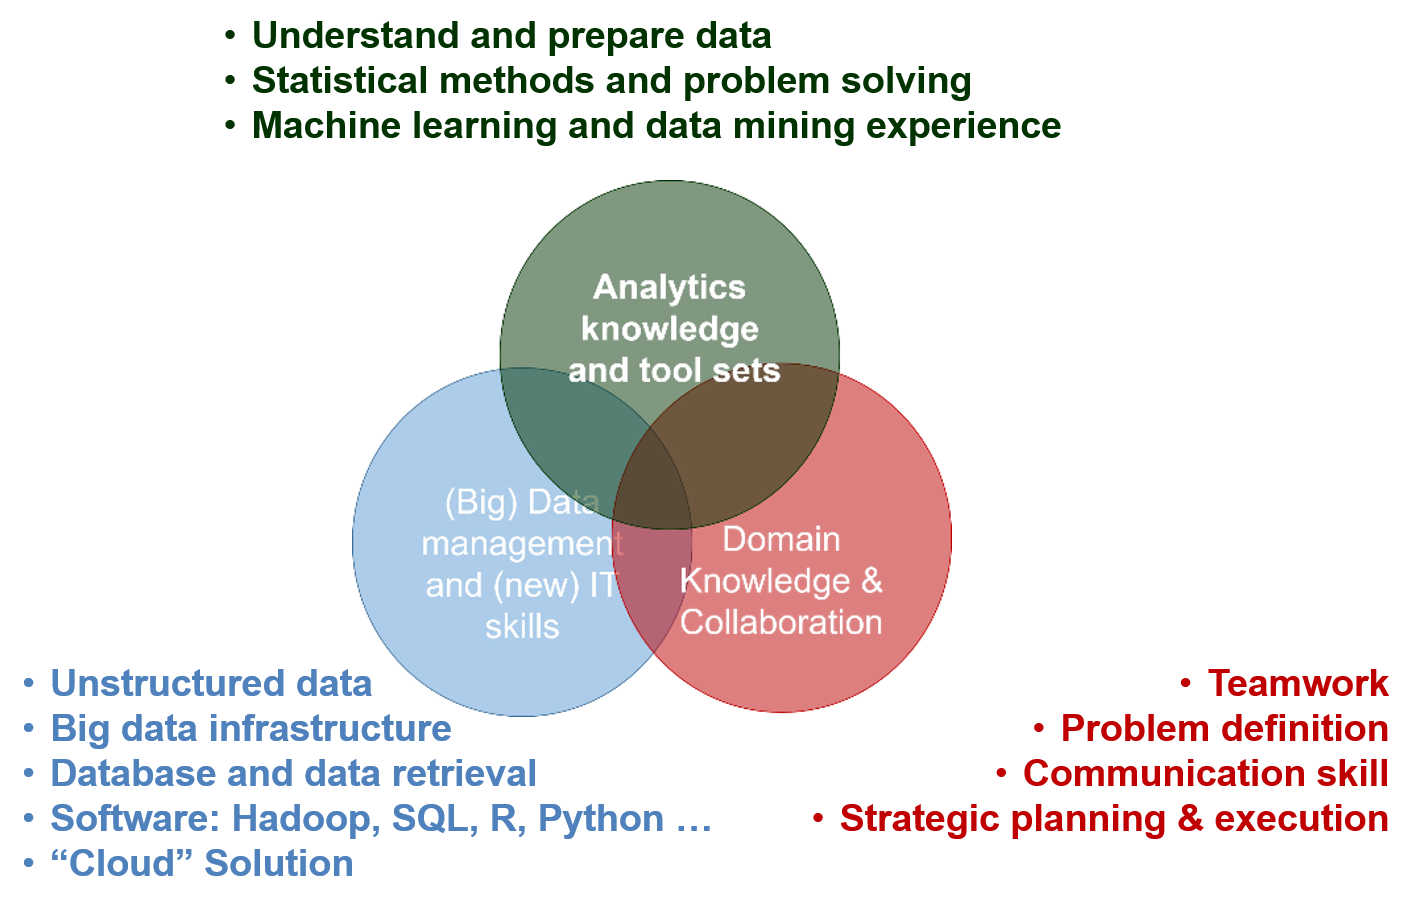
\includegraphics{images/softskill2.png}

\section{Common Pitfalls of Data Science
Projects}\label{common-pitfalls-of-data-science-projects}

Data science projects are usually complicated, and many of these data
science projects eventually fail due to various reasons. We will briefly
discuss a few common pitfalls in data science projects and how to avoid
them.

\begin{itemize}
\item
  \textbf{Solve the wrong problem:} data science project usually starts
  with a very vague description and a few rounds of detailed discussion
  with all stakeholders involved are needed to define the busses
  problem. There will be lots of opportunities to introduce misalignment
  when mapping the business problem into specific data science methods.
  Especially when the quality and availability of the data are not as
  good as what is expected at the first place. If not well-communicated
  during the project, the final data science solution may not be the
  right one to solve the business problem. As the data scientist
  (sometimes the only data scientist) in the room, we must understand
  the business problem thoroughly and communicate regularly to business
  partners especially there is a change of status to make sure everyone
  is aligned with the progress and final deliverables.
\item
  \textbf{Over promise on business value:} business leaders usually have
  high expectation on data science projects and the goal of business
  value and deliverables sometimes are set unrealistic and eventually
  beyond the scope of available data and computation resource. As the
  data scientist (sometimes the only data scientist) in the room, we
  must have our voice heard based on fact (i.e.~data, analytics, and
  resources) instead of wishful thinking. Backed with fact-based
  evidence, it is easier to communicate what is a realistic goal for the
  entire team.
\item
  \textbf{Too optimistic about the timeline:} there are lots of
  uncertainties in data science projects such as the data source
  availability and data quality, computation hardware and software,
  resource availability in the business team, implementation team and IT
  department, as well as project direction change which may delay the
  final delivery date. To have a better-estimated timeline, get as much
  detail as possible for all the needed tasks and estimated each task
  individually and reach out to each team member to confirm their
  availability. Most importantly, communicate with the entire team if
  there are blocking factors for the project in a prompt way such that
  everyone aware of the situation and potential impact on the timeline.
\item
  \textbf{Too optimistic about data availability and quality:} the most
  important asset in data science project is data. Even though we are at
  the big data age, often there is not enough relevant data for the data
  science projects. The data quality is also a general problem for data
  science projects. A thorough data availability and quality check are
  needed at the beginning of the data science project to estimate the
  needed effort to obtain data as well as data cleaning.
\item
  \textbf{Model cannot be scaled:} be careful if you use a subset of
  data to fit the model and then scale it to the entire dataset. When
  developing the model using a smaller dataset, we must keep in mind how
  much computation resources needed for the whole dataset. With limited
  computation resource, it is important to maximize the computation time
  in production to a reasonable level based on the business application
  when fits the model with a sample dataset.
\item
  \textbf{Take too long to fail:} data science projects usually are
  trying to push the boundary of current applications to new territory,
  people do not expect all data science projects to be successful. Fail
  fast is good practice such that we can quickly find a better way to
  solve the problem. A data scientist needs to have an open mindset to
  not stuck with one idea or one approach for a long time to avoid
  taking too long to fail.
\end{itemize}

\chapter{Introduction to the data}\label{introduction-to-the-data}

Before tackling analytics problem, we start by introducing data to be
analyzed in later chapters.

\section{Customer Data for Clothing
Company}\label{customer-data-for-clothing-company}

Our first data set represents customers of a clothing company who sells
products in stores and online. This data is typical of what one might
get from a company's marketing data base (the data base will have more
data than the one we show here). This data includes 1000 customers for
whom we have 3 types of data:

\begin{enumerate}
\def\labelenumi{\arabic{enumi}.}
\tightlist
\item
  Demography

  \begin{itemize}
  \tightlist
  \item
    \texttt{age}: age of the respondent
  \item
    \texttt{gender}: male/female
  \item
    \texttt{house}: 0/1 variable indicating if the customer owns a house
    or not
  \end{itemize}
\item
  Sales in the past year

  \begin{itemize}
  \tightlist
  \item
    \texttt{store\_exp}: expense in store
  \item
    \texttt{online\_exp}: expense online
  \item
    \texttt{store\_trans}: times of store purchase
  \item
    \texttt{online\_trans}: times of online purchase
  \end{itemize}
\item
  Survey on product preference
\end{enumerate}

It is common for companies to survey their customers and draw insights
to guide future marketing activities. The survey is as below:

How strongly do you agree or disagree with the following statements:

\begin{enumerate}
\def\labelenumi{\arabic{enumi}.}
\tightlist
\item
  Strong disagree
\item
  Disagree
\item
  Neither agree nor disagree
\item
  Agree
\item
  Strongly agree
\end{enumerate}

\begin{itemize}
\tightlist
\item
  Q1. I like to buy clothes from different brands
\item
  Q2. I buy almost all my clothes from some of my favorite brands
\item
  Q3. I like to buy premium brands
\item
  Q4. Quality is the most important factor in my purchasing decision
\item
  Q5. Style is the most important factor in my purchasing decision
\item
  Q6. I prefer to buy clothes in store
\item
  Q7. I prefer to buy clothes online
\item
  Q8. Price is important
\item
  Q9. I like to try different styles
\item
  Q10. I like to make a choice by myself and don't need too much of
  others' suggestions
\end{itemize}

There are 4 segments of customers:

\begin{enumerate}
\def\labelenumi{\arabic{enumi}.}
\tightlist
\item
  Price
\item
  Conspicuous
\item
  Quality
\item
  Style
\end{enumerate}

Let's check it:

\begin{Shaded}
\begin{Highlighting}[]
\KeywordTok{str}\NormalTok{(sim.dat,}\DataTypeTok{vec.len=}\DecValTok{3}\NormalTok{)}
\end{Highlighting}
\end{Shaded}

\begin{verbatim}
## 'data.frame':    1000 obs. of  19 variables:
##  $ age         : int  57 63 59 60 51 59 57 57 ...
##  $ gender      : Factor w/ 2 levels "Female","Male": 1 1 2 2 2 2 2 2 ...
##  $ income      : num  120963 122008 114202 113616 ...
##  $ house       : Factor w/ 2 levels "No","Yes": 2 2 2 2 2 2 2 2 ...
##  $ store_exp   : num  529 478 491 348 ...
##  $ online_exp  : num  304 110 279 142 ...
##  $ store_trans : int  2 4 7 10 4 4 5 11 ...
##  $ online_trans: int  2 2 2 2 4 5 3 5 ...
##  $ Q1          : int  4 4 5 5 4 4 4 5 ...
##  $ Q2          : int  2 1 2 2 1 2 1 2 ...
##  $ Q3          : int  1 1 1 1 1 1 1 1 ...
##  $ Q4          : int  2 2 2 3 3 2 2 3 ...
##  $ Q5          : int  1 1 1 1 1 1 1 1 ...
##  $ Q6          : int  4 4 4 4 4 4 4 4 ...
##  $ Q7          : int  1 1 1 1 1 1 1 1 ...
##  $ Q8          : int  4 4 4 4 4 4 4 4 ...
##  $ Q9          : int  2 1 1 2 2 1 1 2 ...
##  $ Q10         : int  4 4 4 4 4 4 4 4 ...
##  $ segment     : Factor w/ 4 levels "Conspicuous",..: 2 2 2 2 2 2 2 2 ...
\end{verbatim}

\section{Customer Satisfaction Survey Data from Airline
Company}\label{customer-satisfaction-survey-data-from-airline-company}

This data set is from a customer satisfaction survey for three airline
companies. There are \texttt{N=1000} respondents and 15 questions. The
market researcher asked respondents to recall the experience with
different airline companies and assign a score (1-9) to each airline
company for all the 15 questions. The higher the score, the more
satisfied the customer to the specific item. The 15 questions are of 4
types (the variable names are in the parentheses):

\begin{itemize}
\tightlist
\item
  How satisfied are you with your\_\_\_\_\_\_?
\end{itemize}

\begin{enumerate}
\def\labelenumi{\arabic{enumi}.}
\tightlist
\item
  Ticketing

  \begin{itemize}
  \tightlist
  \item
    Ease of making reservation(Easy\_Reservation)
  \item
    Availability of preferred seats(Preferred\_Seats)
  \item
    Variety of flight options(Flight\_Options)
  \item
    Ticket prices(Ticket\_Prices)
  \end{itemize}
\item
  Aircraft

  \begin{itemize}
  \tightlist
  \item
    Seat comfort(Seat\_Comfort)
  \item
    Roominess of seat area(Seat\_Roominess)
  \item
    Availability of Overhead(Overhead\_Storage)
  \item
    Cleanliness of aircraft(Clean\_Aircraft)
  \end{itemize}
\item
  Service

  \begin{itemize}
  \tightlist
  \item
    Courtesy of flight attendant(Courtesy)
  \item
    Friendliness(Friendliness)
  \item
    Helpfulness(Helpfulness)
  \item
    Food and drinks(Service)
  \end{itemize}
\item
  General

  \begin{itemize}
  \tightlist
  \item
    Overall satisfaction(Satisfaction)
  \item
    Purchase again(Fly\_Again)
  \item
    Willingness to recommend(Recommend)
  \end{itemize}
\end{enumerate}

Now check the data frame we have:

\begin{Shaded}
\begin{Highlighting}[]
\KeywordTok{str}\NormalTok{(rating,}\DataTypeTok{vec.len=}\DecValTok{3}\NormalTok{)}
\end{Highlighting}
\end{Shaded}

\begin{verbatim}
## Classes 'tbl_df', 'tbl' and 'data.frame':    3000 obs. of  17 variables:
##  $ Easy_Reservation: int  6 5 6 5 4 5 6 4 ...
##  $ Preferred_Seats : int  5 7 6 6 5 6 6 6 ...
##  $ Flight_Options  : int  4 7 5 5 3 4 6 3 ...
##  $ Ticket_Prices   : int  5 6 6 5 6 5 5 5 ...
##  $ Seat_Comfort    : int  5 6 7 7 6 6 6 4 ...
##  $ Seat_Roominess  : int  7 8 6 8 7 8 6 5 ...
##  $ Overhead_Storage: int  5 5 7 6 5 4 4 4 ...
##  $ Clean_Aircraft  : int  7 6 7 7 7 7 6 4 ...
##  $ Courtesy        : int  5 6 6 4 2 5 5 4 ...
##  $ Friendliness    : int  4 6 6 6 3 4 5 5 ...
##  $ Helpfulness     : int  6 5 6 4 4 5 5 4 ...
##  $ Service         : int  6 5 6 5 3 5 5 5 ...
##  $ Satisfaction    : int  6 7 7 5 4 6 5 5 ...
##  $ Fly_Again       : int  6 6 6 7 4 5 3 4 ...
##  $ Recommend       : int  3 6 5 5 4 5 6 5 ...
##  $ ID              : int  1 2 3 4 5 6 7 8 ...
##  $ Airline         : chr  "AirlineCo.1" "AirlineCo.1" "AirlineCo.1" ...
\end{verbatim}

\chapter{Data Pre-processing}\label{data-pre-processing}

Many data analysis related books focus on models, algorithms and
statistical inferences. However, in practice, raw data is usually not
directly used for modeling. Data preprocessing is the process of
converting raw data into clean data that is proper for modeling. A model
fails for various reasons. One is that the modeler doesn't correctly
preprocess data before modeling. Data preprocessing can significantly
impact model results, such as imputing missing value and handling with
outliers. So data preprocessing is a very critical part.

\begin{figure}[htbp]
\centering
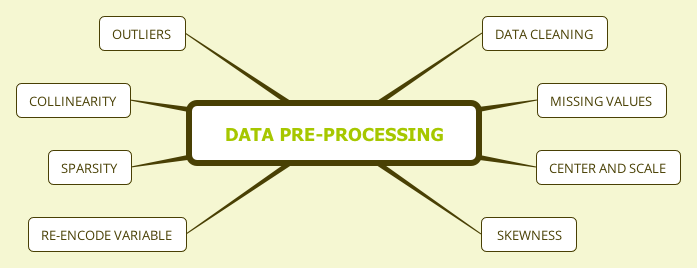
\includegraphics[width=0.90000\textwidth]{images/DataPre-processing.png}
\caption{Data Pre-processing Outline}
\end{figure}

In real life, depending on the stage of data cleanup, data has the
following types:

\begin{enumerate}
\def\labelenumi{\arabic{enumi}.}
\tightlist
\item
  Raw data
\item
  Technically correct data
\item
  Data that is proper for the model
\item
  Summarized data
\item
  Data with fixed format
\end{enumerate}

The raw data is the first-hand data that analysts pull from the
database, market survey responds from your clients, the experimental
results collected by the R \& D department, and so on. These data may be
very rough, and R sometimes can't read them directly. The table title
could be multi-line, or the format does not meet the requirements:

\begin{itemize}
\tightlist
\item
  Use 50\% to represent the percentage rather than 0.5, so R will read
  it as a character;
\item
  The missing value of the sales is represented by ``-'' instead of
  space so that R will treat the variable as character or factor type;
\item
  The data is in a slideshow document, or the spreadsheet is not
  ``.csv'' but ``.xlsx''
\item
  \ldots{}
\end{itemize}

Most of the time, you need to clean the data so that R can import them.
Some data format requires a specific package. Technically correct data
is the data, after preliminary cleaning or format conversion, that R (or
another tool you use) can successfully import it.

Assume we have loaded the data into R with reasonable column names,
variable format and so on. That does not mean the data is entirely
correct. There may be some observations that do not make sense, such as
age is negative, the discount percentage is greater than 1, or data is
missing. Depending on the situation, there may be a variety of problems
with the data. It is necessary to clean the data before modeling.
Moreover, different models have different requirements on the data. For
example, some model may require the variables are of consistent scale;
some may be susceptible to outliers or collinearity, some may not be
able to handle categorical variables and so on. The modeler has to
preprocess the data to make it proper for the specific model.

Sometimes we need to aggregate the data. For example, add up the daily
sales to get annual sales of a product at different locations. In
customer segmentation, it is common practice to build a profile for each
segment. It requires calculating some statistics such as average age,
average income, age standard deviation, etc. Data aggregation is also
necessary for presentation, or for data visualization.

The final table results for clients need to be in a nicer format than
what used in the analysis. Usually, data analysts will take the results
from data scientists and adjust the format, such as labels, cell color,
highlight. It is important for a data scientist to make sure the results
look consistent which makes the next step easier for data analysts.

It is highly recommended to store each step of the data and the R code,
making the whole process as repeatable as possible. The R markdown
reproducible report will be extremely helpful for that. If the data
changes, it is easy to rerun the process. In the remainder of this
chapter, we will show the most common data preprocessing methods.

Load the R packages first:

\begin{Shaded}
\begin{Highlighting}[]
\KeywordTok{source}\NormalTok{(}\StringTok{"https://raw.githubusercontent.com/happyrabbit/CE_JSM2017/master/Rcode/00-course-setup.R"}\NormalTok{)}
\end{Highlighting}
\end{Shaded}

\section{Data Cleaning}\label{data-cleaning}

After you load the data, the first thing is to check how many variables
are there, the type of variables, the distributions, and data errors.
Let's read and check the data:

\begin{Shaded}
\begin{Highlighting}[]
\NormalTok{sim.dat <-}\StringTok{ }\KeywordTok{read.csv}\NormalTok{(}\StringTok{"https://raw.githubusercontent.com/happyrabbit/DataScientistR/master/Data/SegData.csv "}\NormalTok{)}
\KeywordTok{summary}\NormalTok{(sim.dat)}
\end{Highlighting}
\end{Shaded}

\begin{verbatim}
##       age           gender        income      
##  Min.   : 16.0   Female:554   Min.   : 41776  
##  1st Qu.: 25.0   Male  :446   1st Qu.: 85832  
##  Median : 36.0                Median : 93869  
##  Mean   : 38.8                Mean   :113543  
##  3rd Qu.: 53.0                3rd Qu.:124572  
##  Max.   :300.0                Max.   :319704  
##                               NA's   :184     
##  house       store_exp       online_exp  
##  No :432   Min.   : -500   Min.   :  69  
##  Yes:568   1st Qu.:  205   1st Qu.: 420  
##            Median :  329   Median :1942  
##            Mean   : 1357   Mean   :2120  
##            3rd Qu.:  597   3rd Qu.:2441  
##            Max.   :50000   Max.   :9479  
##                                          
##   store_trans     online_trans        Q1     
##  Min.   : 1.00   Min.   : 1.0   Min.   :1.0  
##  1st Qu.: 3.00   1st Qu.: 6.0   1st Qu.:2.0  
##  Median : 4.00   Median :14.0   Median :3.0  
##  Mean   : 5.35   Mean   :13.6   Mean   :3.1  
##  3rd Qu.: 7.00   3rd Qu.:20.0   3rd Qu.:4.0  
##  Max.   :20.00   Max.   :36.0   Max.   :5.0  
##                                              
##        Q2             Q3             Q4      
##  Min.   :1.00   Min.   :1.00   Min.   :1.00  
##  1st Qu.:1.00   1st Qu.:1.00   1st Qu.:2.00  
##  Median :1.00   Median :1.00   Median :3.00  
##  Mean   :1.82   Mean   :1.99   Mean   :2.76  
##  3rd Qu.:2.00   3rd Qu.:3.00   3rd Qu.:4.00  
##  Max.   :5.00   Max.   :5.00   Max.   :5.00  
##                                              
##        Q5             Q6             Q7      
##  Min.   :1.00   Min.   :1.00   Min.   :1.00  
##  1st Qu.:1.75   1st Qu.:1.00   1st Qu.:2.50  
##  Median :4.00   Median :2.00   Median :4.00  
##  Mean   :2.94   Mean   :2.45   Mean   :3.43  
##  3rd Qu.:4.00   3rd Qu.:4.00   3rd Qu.:4.00  
##  Max.   :5.00   Max.   :5.00   Max.   :5.00  
##                                              
##        Q8            Q9            Q10      
##  Min.   :1.0   Min.   :1.00   Min.   :1.00  
##  1st Qu.:1.0   1st Qu.:2.00   1st Qu.:1.00  
##  Median :2.0   Median :4.00   Median :2.00  
##  Mean   :2.4   Mean   :3.08   Mean   :2.32  
##  3rd Qu.:3.0   3rd Qu.:4.00   3rd Qu.:3.00  
##  Max.   :5.0   Max.   :5.00   Max.   :5.00  
##                                             
##         segment   
##  Conspicuous:200  
##  Price      :250  
##  Quality    :200  
##  Style      :350  
##                   
##                   
## 
\end{verbatim}

Are there any problems? Questionnaire response Q1-Q10 seem reasonable,
the minimum is 1 and maximum is 5. Recall that the questionnaire score
is 1-5. The number of store transactions (store\_trans) and online
transactions (store\_trans) make sense too. Things need to pay attention
are:

\begin{itemize}
\tightlist
\item
  There are some missing values.
\item
  There are outliers for store expenses (\texttt{store\_exp}). The
  maximum value is 50000. Who would spend \$50000 a year buying clothes?
  Is it an imputation error?
\item
  There is a negative value ( -500) in \texttt{store\_exp} which is not
  logical.
\item
  Someone is 300 years old.
\end{itemize}

How to deal with that? Depending on the real situation, if the sample
size is large enough, it will not hurt to delete those problematic
samples. Here we have 1000 observations. Since marketing survey is
usually expensive, it is better to set these values as missing and
impute them instead of deleting the rows.

\begin{Shaded}
\begin{Highlighting}[]
\CommentTok{# set problematic values as missings}
\NormalTok{sim.dat$age[}\KeywordTok{which}\NormalTok{(sim.dat$age>}\DecValTok{100}\NormalTok{)]<-}\OtherTok{NA}
\NormalTok{sim.dat$store_exp[}\KeywordTok{which}\NormalTok{(sim.dat$store_exp<}\DecValTok{0}\NormalTok{)]<-}\OtherTok{NA}
\CommentTok{# see the results}
\KeywordTok{summary}\NormalTok{(}\KeywordTok{subset}\NormalTok{(sim.dat,}\DataTypeTok{select=}\KeywordTok{c}\NormalTok{(}\StringTok{"age"}\NormalTok{,}\StringTok{"income"}\NormalTok{)))}
\end{Highlighting}
\end{Shaded}

\begin{verbatim}
##       age           income      
##  Min.   :16.0   Min.   : 41776  
##  1st Qu.:25.0   1st Qu.: 85832  
##  Median :36.0   Median : 93869  
##  Mean   :38.6   Mean   :113543  
##  3rd Qu.:53.0   3rd Qu.:124572  
##  Max.   :69.0   Max.   :319704  
##  NA's   :1      NA's   :184
\end{verbatim}

Now we will deal with the missing values in the data.

\section{Missing Values}\label{missing-values}

You can write a whole book about missing value. This section will only
show some of the most commonly used methods without getting too deep
into the topic. Chapter 7 of the book by De Waal, Pannekoek and Scholtus
\citep{Ton2011} makes a concise overview of some of the existing
imputation methods. The choice of specific method depends on the actual
situation. There is no best way.

One question to ask before imputation: Is there any auxiliary
information? Being aware of any auxiliary information is critical. For
example, if the system set customer who did not purchase as missing,
then the real purchasing amount should be 0. Is missing a random
occurrence? If so, it may be reasonable to impute with mean or median.
If not, is there a potential mechanism for the missing data? For
example, older people are more reluctant to disclose their ages in the
questionnaire, so that the absence of age is not completely random. In
this case, the missing values need to be estimated using the
relationship between age and other independent variables. For example,
use variables such as whether they have children, income, and other
survey questions to build a model to predict age.

Also, the purpose of modeling is important for selecting imputation
methods. If the goal is to interpret the parameter estimate or
statistical inference, then it is important to study the missing
mechanism carefully and to estimate the missing values using non-missing
information as much as possible. If the goal is to predict, people
usually will not study the absence mechanism rigorously (but sometimes
the mechanism is obvious). If the absence mechanism is not clear, treat
it as missing at random and use mean, median, or k-nearest neighbor to
impute. Since statistical inference is sensitive to missing values,
researchers from survey statistics have conducted in-depth studies of
various imputation schemes which focus on valid statistical inference.
The problem of missing values in the prediction model is different from
that in the traditional survey. Therefore, there are not many papers on
missing value imputation in the prediction model. Those who want to
study further can refer to Saar-Tsechansky and Provost's comparison of
different imputation methods \citep{missing1} and De Waal, Pannekoek and
Scholtus' book \citep{Ton2011}.

\subsection{Impute missing values with
median/mode}\label{impute-missing-values-with-medianmode}

In the case of missing at random, a common method is to impute with the
mean (continuous variable) or median (categorical variables). You can
use \texttt{impute()} function in \texttt{imputeMissings} package.

\begin{Shaded}
\begin{Highlighting}[]
\CommentTok{# save the result as another object}
\NormalTok{demo_imp<-}\KeywordTok{impute}\NormalTok{(sim.dat,}\DataTypeTok{method=}\StringTok{"median/mode"}\NormalTok{)}
\CommentTok{# check the first 5 columns, there is no missing values in other columns}
\KeywordTok{summary}\NormalTok{(demo_imp[,}\DecValTok{1}\NormalTok{:}\DecValTok{5}\NormalTok{])}
\end{Highlighting}
\end{Shaded}

\begin{verbatim}
##       age          gender        income      
##  Min.   :16.0   Female:554   Min.   : 41776  
##  1st Qu.:25.0   Male  :446   1st Qu.: 87896  
##  Median :36.0                Median : 93869  
##  Mean   :38.6                Mean   :109923  
##  3rd Qu.:53.0                3rd Qu.:119456  
##  Max.   :69.0                Max.   :319704  
##  house       store_exp    
##  No :432   Min.   :  156  
##  Yes:568   1st Qu.:  205  
##            Median :  330  
##            Mean   : 1358  
##            3rd Qu.:  597  
##            Max.   :50000
\end{verbatim}

After imputation, \texttt{demo\_imp} has no missing value. This method
is straightforward and widely used. The disadvantage is that it does not
take into account the relationship between the variables. When there is
a significant proportion of missing, it will distort the data. In this
case, it is better to consider the relationship between variables and
study the missing mechanism. In the example here, the missing variables
are numeric. If the missing variable is a categorical/factor variable,
the \texttt{impute()} function will impute with the mode.

You can also use \texttt{preProcess()} function, but it is only for
numeric variables, and can not impute categorical variables. Since
missing values here are numeric, we can use the \texttt{preProcess()}
function. The result is the same as the \texttt{impute()} function.
\texttt{PreProcess()} is a powerful function that can link to a variety
of data preprocessing methods. We will use the function later for other
data preprocessing.

\begin{Shaded}
\begin{Highlighting}[]
\NormalTok{imp<-}\KeywordTok{preProcess}\NormalTok{(sim.dat,}\DataTypeTok{method=}\StringTok{"medianImpute"}\NormalTok{)}
\NormalTok{demo_imp2<-}\KeywordTok{predict}\NormalTok{(imp,sim.dat)}
\KeywordTok{summary}\NormalTok{(demo_imp2[,}\DecValTok{1}\NormalTok{:}\DecValTok{5}\NormalTok{])}
\end{Highlighting}
\end{Shaded}

\begin{verbatim}
##       age          gender        income      
##  Min.   :16.0   Female:554   Min.   : 41776  
##  1st Qu.:25.0   Male  :446   1st Qu.: 87896  
##  Median :36.0                Median : 93869  
##  Mean   :38.6                Mean   :109923  
##  3rd Qu.:53.0                3rd Qu.:119456  
##  Max.   :69.0                Max.   :319704  
##  house       store_exp    
##  No :432   Min.   :  156  
##  Yes:568   1st Qu.:  205  
##            Median :  330  
##            Mean   : 1358  
##            3rd Qu.:  597  
##            Max.   :50000
\end{verbatim}

\subsection{K-nearest neighbors}\label{k-nearest-neighbors}

K-nearest neighbor (KNN) will find the k closest samples (Euclidian
distance) in the training set and impute the mean of those
``neighbors.''

Use \texttt{preProcess()} to conduct KNN:

\begin{Shaded}
\begin{Highlighting}[]
\NormalTok{imp<-}\KeywordTok{preProcess}\NormalTok{(sim.dat,}\DataTypeTok{method=}\StringTok{"knnImpute"}\NormalTok{,}\DataTypeTok{k=}\DecValTok{5}\NormalTok{)}
\CommentTok{# need to use predict() to get KNN result}
\NormalTok{demo_imp<-}\KeywordTok{predict}\NormalTok{(imp,sim.dat)}
\end{Highlighting}
\end{Shaded}

\begin{verbatim}
Error in `[.data.frame`(old, , non_missing_cols, drop = FALSE) : 
  undefined columns selected
\end{verbatim}

Now we get an error saying ``undefined columns selected.'' It is because
\texttt{sim.dat} has non-numeric variables. The \texttt{preProcess()} in
the first line will automatically ignore non-numeric columns, so there
is no error. However, there is a problem when using \texttt{predict()}
to get the result. Removing those variable will solve the problem.

\begin{Shaded}
\begin{Highlighting}[]
\CommentTok{# find factor columns}
\NormalTok{imp<-}\KeywordTok{preProcess}\NormalTok{(sim.dat,}\DataTypeTok{method=}\StringTok{"knnImpute"}\NormalTok{,}\DataTypeTok{k=}\DecValTok{5}\NormalTok{)}
\NormalTok{idx<-}\KeywordTok{which}\NormalTok{(}\KeywordTok{lapply}\NormalTok{(sim.dat,class)==}\StringTok{"factor"}\NormalTok{)}
\NormalTok{demo_imp<-}\KeywordTok{predict}\NormalTok{(imp,sim.dat[,-idx])}
\KeywordTok{summary}\NormalTok{(demo_imp[,}\DecValTok{1}\NormalTok{:}\DecValTok{3}\NormalTok{])}
\end{Highlighting}
\end{Shaded}

\begin{verbatim}
##       age             income         store_exp     
##  Min.   :-1.591   Min.   :-1.440   Min.   :-0.433  
##  1st Qu.:-0.957   1st Qu.:-0.537   1st Qu.:-0.416  
##  Median :-0.182   Median :-0.376   Median :-0.371  
##  Mean   : 0.000   Mean   : 0.024   Mean   : 0.000  
##  3rd Qu.: 1.016   3rd Qu.: 0.215   3rd Qu.:-0.274  
##  Max.   : 2.144   Max.   : 4.136   Max.   :17.527
\end{verbatim}

\texttt{lapply(data,class)} can return a list of column class. Here the
data frame is \texttt{sim.dat}, and the following code will give the
list of column class:

\begin{Shaded}
\begin{Highlighting}[]
\CommentTok{# only show the first three elements}
\KeywordTok{lapply}\NormalTok{(sim.dat,class)[}\DecValTok{1}\NormalTok{:}\DecValTok{3}\NormalTok{]}
\end{Highlighting}
\end{Shaded}

\begin{verbatim}
## $age
## [1] "integer"
## 
## $gender
## [1] "factor"
## 
## $income
## [1] "numeric"
\end{verbatim}

Comparing the KNN result with the previous median imputation, the two
are very different. This is because when you tell the
\texttt{preProcess()} function to use KNN (the option
\texttt{method\ ="\ knnImpute"}), it will automatically standardize the
data. Another way is to use Bagging tree (in the next section). Note
that KNN can not impute samples with the entire row missing. The reason
is straightforward. Since the algorithm uses the average of its
neighbors if none of them has a value, what does it apply to calculate
the mean? Let's append a new row with all values missing to the original
data frame to get a new object called \texttt{temp}. Then apply KNN to
\texttt{temp} and see what happens:

\begin{Shaded}
\begin{Highlighting}[]
\NormalTok{temp<-}\KeywordTok{rbind}\NormalTok{(sim.dat,}\KeywordTok{rep}\NormalTok{(}\OtherTok{NA}\NormalTok{,}\KeywordTok{ncol}\NormalTok{(sim.dat)))}
\NormalTok{imp<-}\KeywordTok{preProcess}\NormalTok{(sim.dat,}\DataTypeTok{method=}\StringTok{"knnImpute"}\NormalTok{,}\DataTypeTok{k=}\DecValTok{5}\NormalTok{)}
\NormalTok{idx<-}\KeywordTok{which}\NormalTok{(}\KeywordTok{lapply}\NormalTok{(temp,class)==}\StringTok{"factor"}\NormalTok{)}
\end{Highlighting}
\end{Shaded}

\begin{Shaded}
\begin{Highlighting}[]
\NormalTok{demo_imp<-}\KeywordTok{predict}\NormalTok{(imp,temp[,-idx])}
\end{Highlighting}
\end{Shaded}

\begin{verbatim}
Error in FUN(newX[, i], ...) : 
  cannot impute when all predictors are missing in the new data point
\end{verbatim}

There is an error saying ``cannot impute when all predictors are missing
in the new data point''. It is easy to fix by finding and removing the
problematic row:

\begin{Shaded}
\begin{Highlighting}[]
\NormalTok{idx<-}\KeywordTok{apply}\NormalTok{(temp,}\DecValTok{1}\NormalTok{,function(x) }\KeywordTok{sum}\NormalTok{(}\KeywordTok{is.na}\NormalTok{(x)) )}
\KeywordTok{as.vector}\NormalTok{(}\KeywordTok{which}\NormalTok{(idx==}\KeywordTok{ncol}\NormalTok{(temp)))}
\end{Highlighting}
\end{Shaded}

\begin{verbatim}
## [1] 1001
\end{verbatim}

It shows that row 1001 is problematic. You can go ahead to delete it.

\subsection{Bagging Tree}\label{bagging-tree}

Bagging (Bootstrap aggregating) was originally proposed by Leo Breiman.
It is one of the earliest ensemble methods \citep{bag1}. When used in
missing value imputation, it will use the remaining variables as
predictors to train a bagging tree and then use the tree to predict the
missing values. Although theoretically, the method is powerful, the
computation is much more intense than KNN. In practice, there is a
trade-off between computation time and the effect. If a median or mean
meet the modeling needs, even bagging tree may improve the accuracy a
little, but the upgrade is so marginal that it does not deserve the
extra time. The bagging tree itself is a model for regression and
classification. Here we use \texttt{preProcess()} to impute
\texttt{sim.dat}:

\begin{Shaded}
\begin{Highlighting}[]
\NormalTok{imp<-}\KeywordTok{preProcess}\NormalTok{(sim.dat,}\DataTypeTok{method=}\StringTok{"bagImpute"}\NormalTok{)}
\NormalTok{demo_imp<-}\KeywordTok{predict}\NormalTok{(imp,sim.dat)}
\KeywordTok{summary}\NormalTok{(demo_imp[,}\DecValTok{1}\NormalTok{:}\DecValTok{5}\NormalTok{])}
\end{Highlighting}
\end{Shaded}

\begin{verbatim}
      age           gender        income       house       store_exp      
 Min.   :16.00   Female:554   Min.   : 41776   No :432   Min.   :  155.8  
 1st Qu.:25.00   Male  :446   1st Qu.: 86762   Yes:568   1st Qu.:  205.1  
 Median :36.00                Median : 94739             Median :  329.0  
 Mean   :38.58                Mean   :114665             Mean   : 1357.7  
 3rd Qu.:53.00                3rd Qu.:123726             3rd Qu.:  597.3  
 Max.   :69.00                Max.   :319704             Max.   :50000.0  
\end{verbatim}

\section{Centering and Scaling}\label{centering-and-scaling}

It is the most straightforward data transformation. It centers and
scales a variable to mean 0 and standard deviation 1. It ensures that
the criterion for finding linear combinations of the predictors is based
on how much variation they explain and therefore improves the numerical
stability. Models involving finding linear combinations of the
predictors to explain response/predictors variation need data centering
and scaling, such as PCA \citep{pca1}, PLS \citep{PLS1} and EFA
\citep{EFA1}. You can quickly write code yourself to conduct this
transformation.

Let's standardize the variable \texttt{income} from \texttt{sim.dat}:

\begin{Shaded}
\begin{Highlighting}[]
\NormalTok{income<-sim.dat$income}
\CommentTok{# calculate the mean of income}
\NormalTok{mux<-}\KeywordTok{mean}\NormalTok{(income,}\DataTypeTok{na.rm=}\NormalTok{T)}
\CommentTok{# calculate the standard deviation of income}
\NormalTok{sdx<-}\KeywordTok{sd}\NormalTok{(income,}\DataTypeTok{na.rm=}\NormalTok{T)}
\CommentTok{# centering}
\NormalTok{tr1<-income-mux}
\CommentTok{# scaling}
\NormalTok{tr2<-tr1/sdx}
\end{Highlighting}
\end{Shaded}

Or the function \texttt{preProcess()} in package \texttt{caret} can
apply this transformation to a set of predictors.

\begin{Shaded}
\begin{Highlighting}[]
\NormalTok{sdat<-}\KeywordTok{subset}\NormalTok{(sim.dat,}\DataTypeTok{select=}\KeywordTok{c}\NormalTok{(}\StringTok{"age"}\NormalTok{,}\StringTok{"income"}\NormalTok{))}
\CommentTok{# set the "method" option}
\NormalTok{trans<-}\KeywordTok{preProcess}\NormalTok{(sdat,}\DataTypeTok{method=}\KeywordTok{c}\NormalTok{(}\StringTok{"center"}\NormalTok{,}\StringTok{"scale"}\NormalTok{))}
\CommentTok{# use predict() function to get the final result}
\NormalTok{transformed<-}\KeywordTok{predict}\NormalTok{(trans,sdat)}
\end{Highlighting}
\end{Shaded}

Now the two variables are in the same scale:

\begin{Shaded}
\begin{Highlighting}[]
\KeywordTok{summary}\NormalTok{(transformed)}
\end{Highlighting}
\end{Shaded}

\begin{verbatim}
##       age             income     
##  Min.   :-1.591   Min.   :-1.44  
##  1st Qu.:-0.957   1st Qu.:-0.56  
##  Median :-0.182   Median :-0.39  
##  Mean   : 0.000   Mean   : 0.00  
##  3rd Qu.: 1.016   3rd Qu.: 0.22  
##  Max.   : 2.144   Max.   : 4.14  
##  NA's   :1        NA's   :184
\end{verbatim}

Sometimes you only need to scale the variable. For example, if the model
adds a penalty to the parameter estimates (such as \(L_2\) penalty is
ridge regression and \(L_1\) penalty in LASSO), the variables need to
have a similar scale to ensure a fair variable selection. I am a heavy
user of this kind of penalty-based model in my work, and I used the
following quantile transformation:

\[
x_{ij}^{*}=\frac{x_{ij}-quantile(x_{.j},0.01)}{quantile(x_{.j}-0.99)-quantile(x_{-j},0.01)}
\]

The reason to use 99\% and 1\% quantile instead of maximum and minimum
values is to resist the impact of outliers.

It is easy to write a function to do it:

\begin{Shaded}
\begin{Highlighting}[]
\NormalTok{qscale<-function(dat)\{}
  \NormalTok{for (i in }\DecValTok{1}\NormalTok{:}\KeywordTok{ncol}\NormalTok{(dat))\{}
    \NormalTok{up<-}\KeywordTok{quantile}\NormalTok{(dat[,i],}\FloatTok{0.99}\NormalTok{)}
    \NormalTok{low<-}\KeywordTok{quantile}\NormalTok{(dat[,i],}\FloatTok{0.01}\NormalTok{)}
    \NormalTok{diff<-up-low}
    \NormalTok{dat[,i]<-(dat[,i]-low)/diff}
  \NormalTok{\}}
  \KeywordTok{return}\NormalTok{(dat)}
\NormalTok{\}}
\end{Highlighting}
\end{Shaded}

In order to illustrate, let's apply it to some variables from
`demo\_imp2:

\begin{Shaded}
\begin{Highlighting}[]
\NormalTok{demo_imp3<-}\KeywordTok{qscale}\NormalTok{(}\KeywordTok{subset}\NormalTok{(demo_imp2,}\DataTypeTok{select=}\KeywordTok{c}\NormalTok{(}\StringTok{"income"}\NormalTok{,}\StringTok{"store_exp"}\NormalTok{,}\StringTok{"online_exp"}\NormalTok{)))}
\KeywordTok{summary}\NormalTok{(demo_imp3)}
\end{Highlighting}
\end{Shaded}

\begin{verbatim}
##      income          store_exp        online_exp     
##  Min.   :-0.0578   Min.   :-0.003   Min.   :-0.0060  
##  1st Qu.: 0.1574   1st Qu.: 0.004   1st Qu.: 0.0427  
##  Median : 0.1852   Median : 0.023   Median : 0.2537  
##  Mean   : 0.2601   Mean   : 0.177   Mean   : 0.2784  
##  3rd Qu.: 0.3046   3rd Qu.: 0.063   3rd Qu.: 0.3229  
##  Max.   : 1.2386   Max.   : 7.477   Max.   : 1.2988
\end{verbatim}

After transformation, most of the variables are between 0-1.

\section{Resolve Skewness}\label{resolve-skewness}

\href{https://en.wikipedia.org/wiki/Skewness}{Skewness} is defined to be
the third standardized central moment. The formula for the sample
skewness statistics is:
\[ skewness=\frac{\sum(x_{i}-\bar{x})^{3}}{(n-1)v^{3/2}}\]
\[v=\frac{\sum(x_{i}-\bar{x})^{2}}{(n-1)}\] Skewness=0 means that the
destribution is symmetric, i.e.~the probability of falling on either
side of the distribution's mean is equal.

\begin{Shaded}
\begin{Highlighting}[]
\CommentTok{# need skewness() function from e1071 package}
\KeywordTok{set.seed}\NormalTok{(}\DecValTok{1000}\NormalTok{)}
\KeywordTok{par}\NormalTok{(}\DataTypeTok{mfrow=}\KeywordTok{c}\NormalTok{(}\DecValTok{1}\NormalTok{,}\DecValTok{2}\NormalTok{),}\DataTypeTok{oma=}\KeywordTok{c}\NormalTok{(}\DecValTok{2}\NormalTok{,}\DecValTok{2}\NormalTok{,}\DecValTok{2}\NormalTok{,}\DecValTok{2}\NormalTok{))}
\CommentTok{# random sample 1000 chi-square distribution with df=2}
\CommentTok{# right skew}
\NormalTok{x1<-}\KeywordTok{rchisq}\NormalTok{(}\DecValTok{1000}\NormalTok{,}\DecValTok{2}\NormalTok{, }\DataTypeTok{ncp =} \DecValTok{0}\NormalTok{)}
\CommentTok{# get left skew variable x2 from x1}
\NormalTok{x2<-}\KeywordTok{max}\NormalTok{(x1)-x1}
\KeywordTok{plot}\NormalTok{(}\KeywordTok{density}\NormalTok{(x2),}\DataTypeTok{main=}\KeywordTok{paste}\NormalTok{(}\StringTok{"left skew, skewnwss ="}\NormalTok{,}\KeywordTok{round}\NormalTok{(}\KeywordTok{skewness}\NormalTok{(x2),}\DecValTok{2}\NormalTok{)), }\DataTypeTok{xlab=}\StringTok{"X2"}\NormalTok{)}
\KeywordTok{plot}\NormalTok{(}\KeywordTok{density}\NormalTok{(x1),}\DataTypeTok{main=}\KeywordTok{paste}\NormalTok{(}\StringTok{"right skew, skewness ="}\NormalTok{,}\KeywordTok{round}\NormalTok{(}\KeywordTok{skewness}\NormalTok{(x1),}\DecValTok{2}\NormalTok{)), }\DataTypeTok{xlab=}\StringTok{"X1"}\NormalTok{)}
\end{Highlighting}
\end{Shaded}

\begin{figure}

{\centering 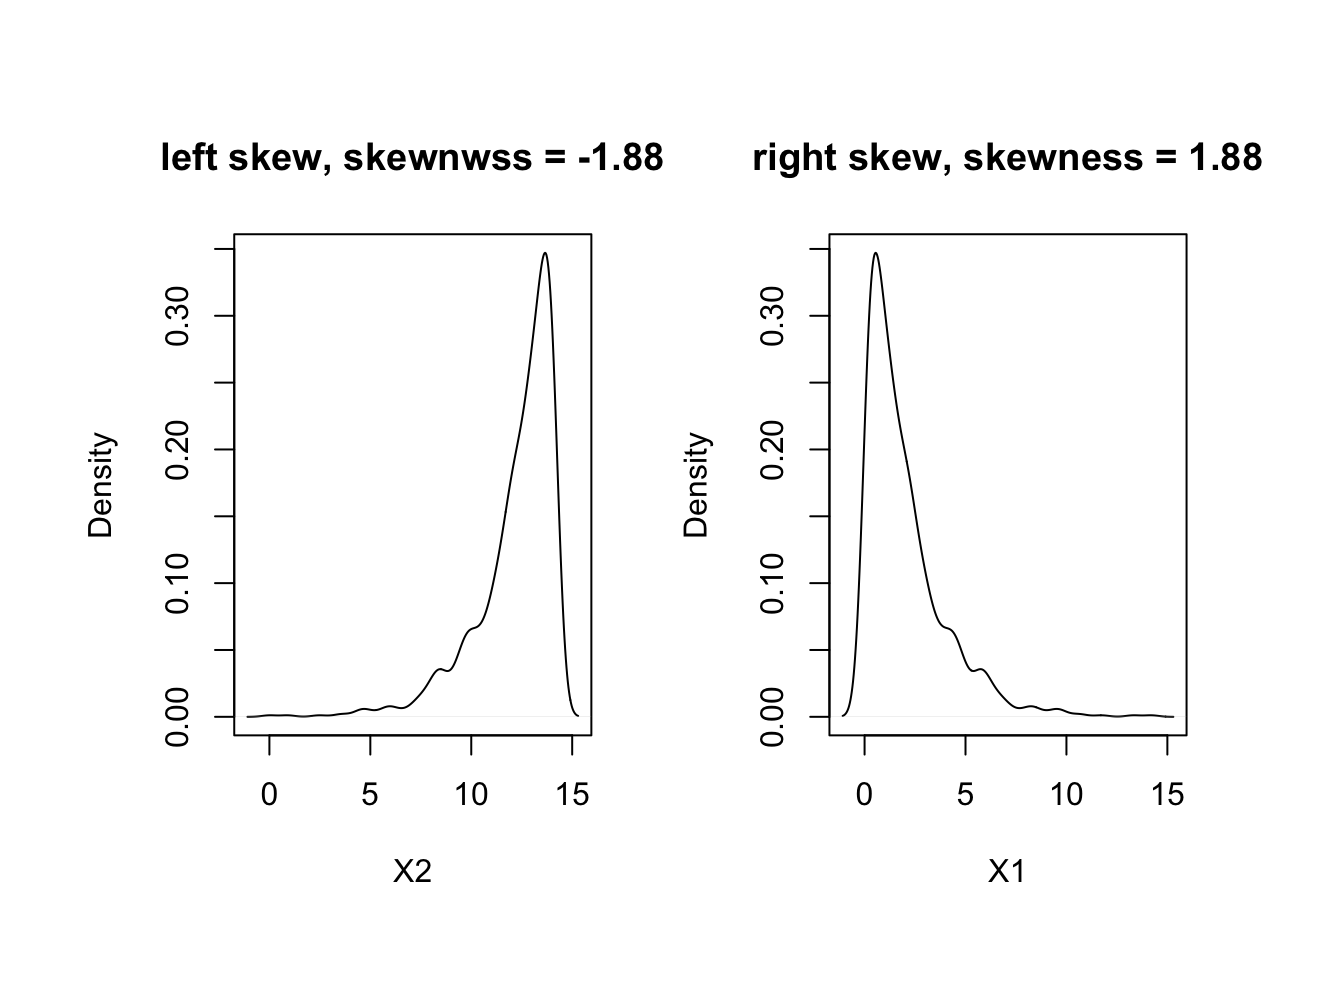
\includegraphics[width=0.8\linewidth]{IDS_files/figure-latex/skew-1} 

}

\caption{Shewed Distribution}\label{fig:skew}
\end{figure}

You can easily tell if a distribution is skewed by simple
visualization(Figure\ref{fig:skew}). There are different ways may help
to remove skewness such as log, square root or inverse. However, it is
often difficult to determine from plots which transformation is most
appropriate for correcting skewness. The Box-Cox procedure automatically
identified a transformation from the family of power transformations
that are indexed by a parameter \(\lambda\)\citep{BOXCOX1}.

\[
x^{*}=\begin{cases}
\begin{array}{c}
\frac{x^{\lambda}-1}{\lambda}\\
log(x)
\end{array} & \begin{array}{c}
if\ \lambda\neq0\\
if\ \lambda=0
\end{array}\end{cases}
\]

It is easy to see that this family includes log transformation
(\(\lambda=0\)), square transformation (\(\lambda=2\)), square root
(\(\lambda=0.5\)), inverse (\(\lambda=-1\)) and others in-between. We
can still use function \texttt{preProcess()} in package \texttt{caret}
to apply this transformation by chaning the \texttt{method} argument.

\begin{Shaded}
\begin{Highlighting}[]
\KeywordTok{describe}\NormalTok{(sim.dat)}
\end{Highlighting}
\end{Shaded}

\begin{verbatim}
##              vars    n      mean       sd  median
## age             1  999     38.58    14.19    36.0
## gender*         2 1000      1.45     0.50     1.0
## income          3  816 113543.07 49842.29 93868.7
## house*          4 1000      1.57     0.50     2.0
## store_exp       5  999   1358.71  2775.17   329.8
## online_exp      6 1000   2120.18  1731.22  1941.9
## store_trans     7 1000      5.35     3.70     4.0
## online_trans    8 1000     13.55     7.96    14.0
## Q1              9 1000      3.10     1.45     3.0
## Q2             10 1000      1.82     1.17     1.0
## Q3             11 1000      1.99     1.40     1.0
## Q4             12 1000      2.76     1.16     3.0
## Q5             13 1000      2.94     1.28     4.0
## Q6             14 1000      2.45     1.44     2.0
## Q7             15 1000      3.43     1.46     4.0
## Q8             16 1000      2.40     1.15     2.0
## Q9             17 1000      3.08     1.12     4.0
## Q10            18 1000      2.32     1.14     2.0
## segment*       19 1000      2.70     1.15     3.0
##                trimmed      mad      min    max  range
## age              37.67    16.31    16.00     69     53
## gender*           1.43     0.00     1.00      2      1
## income       104841.94 28989.47 41775.64 319704 277929
## house*            1.58     0.00     1.00      2      1
## store_exp       845.14   197.47   155.81  50000  49844
## online_exp     1874.51  1015.21    68.82   9479   9411
## store_trans       4.89     2.97     1.00     20     19
## online_trans     13.42    10.38     1.00     36     35
## Q1                3.13     1.48     1.00      5      4
## Q2                1.65     0.00     1.00      5      4
## Q3                1.75     0.00     1.00      5      4
## Q4                2.83     1.48     1.00      5      4
## Q5                3.05     0.00     1.00      5      4
## Q6                2.43     1.48     1.00      5      4
## Q7                3.54     0.00     1.00      5      4
## Q8                2.36     1.48     1.00      5      4
## Q9                3.23     0.00     1.00      5      4
## Q10               2.27     1.48     1.00      5      4
## segment*          2.75     1.48     1.00      4      3
##               skew kurtosis      se
## age           0.47    -1.18    0.45
## gender*       0.22    -1.95    0.02
## income        1.69     2.57 1744.83
## house*       -0.27    -1.93    0.02
## store_exp     8.08   115.04   87.80
## online_exp    1.18     1.31   54.75
## store_trans   1.11     0.69    0.12
## online_trans  0.03    -0.98    0.25
## Q1           -0.12    -1.36    0.05
## Q2            1.13    -0.32    0.04
## Q3            1.06    -0.40    0.04
## Q4           -0.18    -1.46    0.04
## Q5           -0.60    -1.40    0.04
## Q6            0.11    -1.89    0.05
## Q7           -0.90    -0.79    0.05
## Q8            0.21    -1.33    0.04
## Q9           -0.68    -1.10    0.04
## Q10           0.39    -1.23    0.04
## segment*     -0.20    -1.41    0.04
\end{verbatim}

It is easy to see the skewed variables. If \texttt{mean} and
\texttt{trimmed} differ a lot, there is very likely outliers. By
default, \texttt{trimmed} reports mean by dropping the top and bottom
10\%. It can be adjusted by setting argument \texttt{trim=}. It is clear
that \texttt{store\_exp} has outliers.

As an example, we will apply Box-Cox transformation on
\texttt{store\_trans} and \texttt{online\_trans}:

\begin{Shaded}
\begin{Highlighting}[]
\CommentTok{# select the two columns and save them as dat_bc}
\NormalTok{dat_bc<-}\KeywordTok{subset}\NormalTok{(sim.dat,}\DataTypeTok{select=}\KeywordTok{c}\NormalTok{(}\StringTok{"store_trans"}\NormalTok{,}\StringTok{"online_trans"}\NormalTok{))}
\NormalTok{(trans<-}\KeywordTok{preProcess}\NormalTok{(dat_bc,}\DataTypeTok{method=}\KeywordTok{c}\NormalTok{(}\StringTok{"BoxCox"}\NormalTok{)))}
\end{Highlighting}
\end{Shaded}

\begin{verbatim}
## Created from 1000 samples and 2 variables
## 
## Pre-processing:
##   - Box-Cox transformation (2)
##   - ignored (0)
## 
## Lambda estimates for Box-Cox transformation:
## 0.1, 0.7
\end{verbatim}

The last line of the output shows the estimates of \(\lambda\) for each
variable. As before, use \texttt{predict()} to get the transformed
result:

\begin{Shaded}
\begin{Highlighting}[]
\NormalTok{transformed<-}\KeywordTok{predict}\NormalTok{(trans,dat_bc)}
\KeywordTok{par}\NormalTok{(}\DataTypeTok{mfrow=}\KeywordTok{c}\NormalTok{(}\DecValTok{1}\NormalTok{,}\DecValTok{2}\NormalTok{),}\DataTypeTok{oma=}\KeywordTok{c}\NormalTok{(}\DecValTok{2}\NormalTok{,}\DecValTok{2}\NormalTok{,}\DecValTok{2}\NormalTok{,}\DecValTok{2}\NormalTok{))}
\KeywordTok{hist}\NormalTok{(dat_bc$store_trans,}\DataTypeTok{main=}\StringTok{"Before Transformation"}\NormalTok{,}\DataTypeTok{xlab=}\StringTok{"store_trans"}\NormalTok{)}
\KeywordTok{hist}\NormalTok{(transformed$store_trans,}\DataTypeTok{main=}\StringTok{"After Transformation"}\NormalTok{,}\DataTypeTok{xlab=}\StringTok{"store_trans"}\NormalTok{)}
\end{Highlighting}
\end{Shaded}

\begin{figure}

{\centering 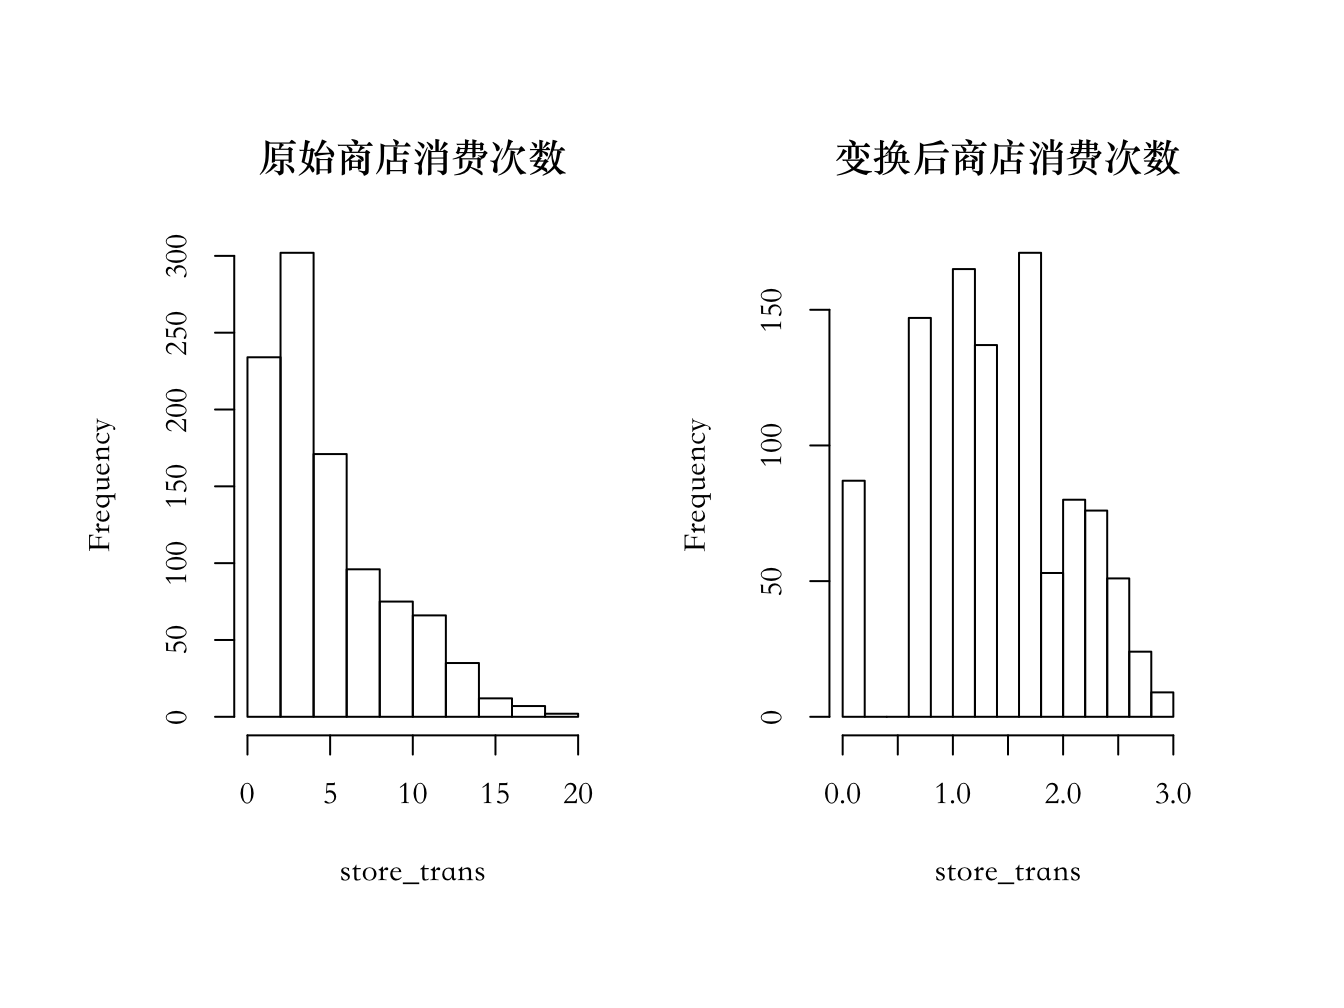
\includegraphics[width=0.8\linewidth]{IDS_files/figure-latex/bc-1} 

}

\caption{Box-Cox Transformation}\label{fig:bc}
\end{figure}

Before the transformation, the \texttt{stroe\_trans} is skewed right.
The situation is significantly improved after (figure\ref{fig:bc}).
\texttt{BoxCoxTrans\ ()} can also conduct Box-Cox transform. But note
that \texttt{BoxCoxTrans\ ()} can only be applied to a single variable,
and it is not possible to transform difference columns in a data frame
at the same time.

\begin{Shaded}
\begin{Highlighting}[]
\NormalTok{(trans<-}\KeywordTok{BoxCoxTrans}\NormalTok{(dat_bc$store_trans))}
\end{Highlighting}
\end{Shaded}

\begin{verbatim}
## Box-Cox Transformation
## 
## 1000 data points used to estimate Lambda
## 
## Input data summary:
##    Min. 1st Qu.  Median    Mean 3rd Qu.    Max. 
##    1.00    3.00    4.00    5.35    7.00   20.00 
## 
## Largest/Smallest: 20 
## Sample Skewness: 1.11 
## 
## Estimated Lambda: 0.1 
## With fudge factor, Lambda = 0 will be used for transformations
\end{verbatim}

\begin{Shaded}
\begin{Highlighting}[]
\NormalTok{transformed<-}\KeywordTok{predict}\NormalTok{(trans,dat_bc$store_trans)}
\KeywordTok{skewness}\NormalTok{(transformed)}
\end{Highlighting}
\end{Shaded}

\begin{verbatim}
## [1] -0.2155
\end{verbatim}

The estimate of \(\lambda\) is the same as before (0.1). The skewness of
the original observation is 1.1, and -0.2 after transformation. Although
it is not strictly 0, it is greatly improved.

\section{Resolve Outliers}\label{resolve-outliers}

Even under certain assumptions we can statistically define outliers, it
can be hard to define in some situations. Box plot, histogram and some
other basic visualizations can be used to initially check whether there
are outliers. For example, we can visualize numerical non-survey
variables in \texttt{sim.dat}:

\begin{Shaded}
\begin{Highlighting}[]
\CommentTok{# select numerical non-survey data}
\NormalTok{sdat<-}\KeywordTok{subset}\NormalTok{(sim.dat,}\DataTypeTok{select=}\KeywordTok{c}\NormalTok{(}\StringTok{"age"}\NormalTok{,}\StringTok{"income"}\NormalTok{,}\StringTok{"store_exp"}\NormalTok{,}\StringTok{"online_exp"}\NormalTok{,}\StringTok{"store_trans"}\NormalTok{,}\StringTok{"online_trans"} \NormalTok{))}
\CommentTok{# use scatterplotMatrix() function from car package}
\KeywordTok{par}\NormalTok{(}\DataTypeTok{oma=}\KeywordTok{c}\NormalTok{(}\DecValTok{2}\NormalTok{,}\DecValTok{2}\NormalTok{,}\DecValTok{1}\NormalTok{,}\DecValTok{2}\NormalTok{))}
\KeywordTok{scatterplotMatrix}\NormalTok{(sdat,}\DataTypeTok{diagonal=}\StringTok{"boxplot"}\NormalTok{,}\DataTypeTok{smoother=}\OtherTok{FALSE}\NormalTok{)}
\end{Highlighting}
\end{Shaded}

\begin{figure}

{\centering 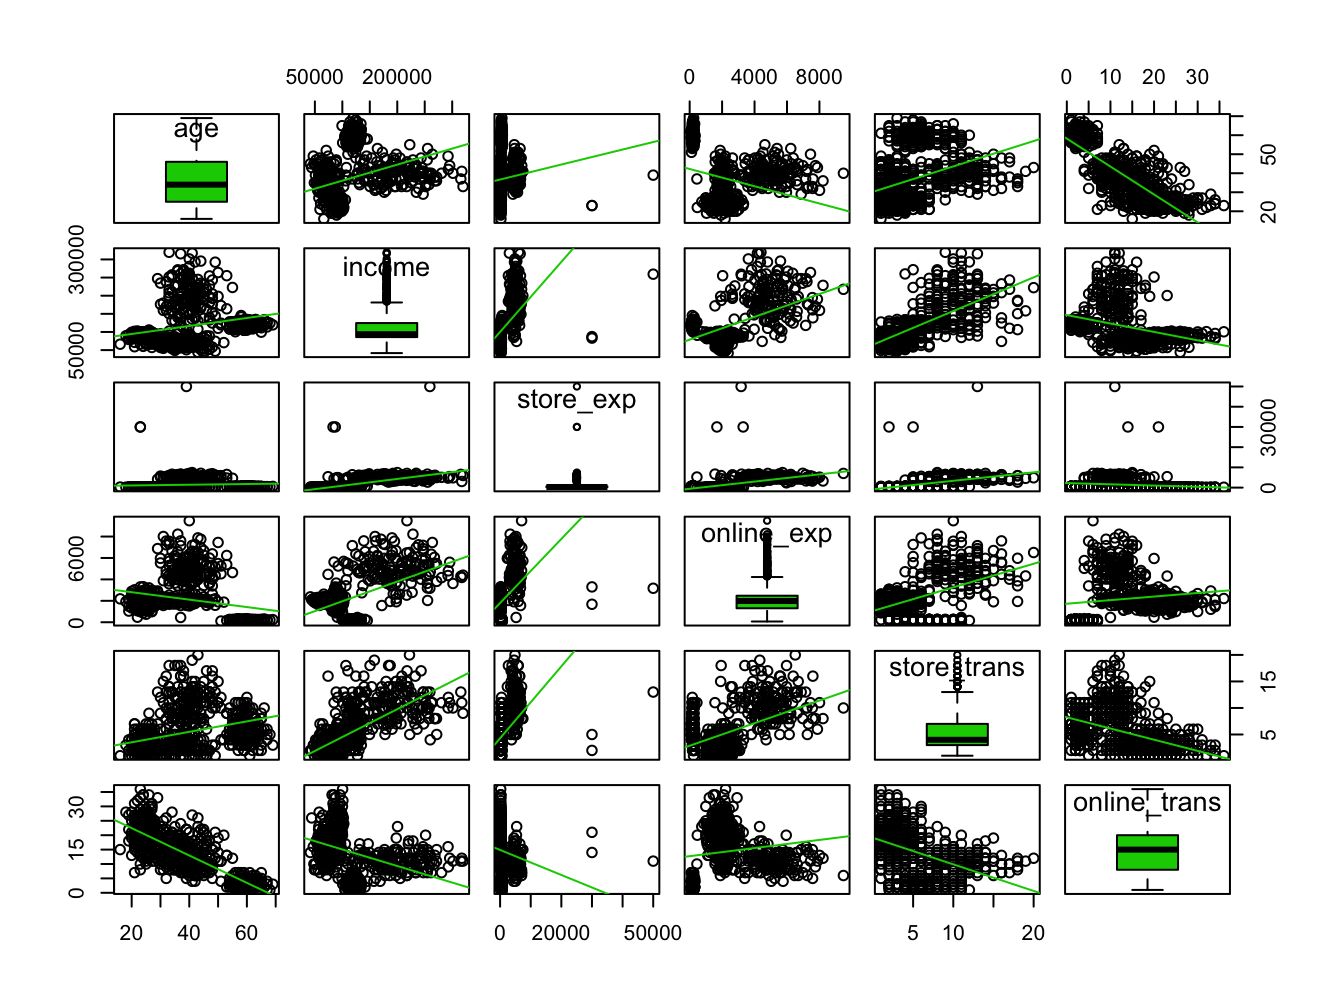
\includegraphics[width=0.8\linewidth]{IDS_files/figure-latex/scm-1} 

}

\caption{Use basic visualization to check outliers}\label{fig:scm}
\end{figure}

As figure \ref{fig:scm} shows, \texttt{store\_exp} has outliers. It is
also easy to observe the pair relationship from the plot. \texttt{age}
is negatively correlated with \texttt{online\_trans} but positively
correlated with \texttt{store\_trans}. It seems that older people tend
to purchase from the local store. The amount of expense is positively
correlated with income. Scatterplot matrix like this can reveal lots of
information before modeling.

In addition to visualization, there are some statistical methods to
define outliers, such as the commonly used Z-score. The Z-score for
variable \(\mathbf{Y}\) is defined as:

\[Z_{i}=\frac{Y_{i}-\bar{Y}}{s}\]

where \(\bar{Y}\) and \(s\) are mean and standard deviation for \(Y\).
Z-score is a measurement of the distance between each observation and
the mean. This method may be misleading, especially when the sample size
is small. Iglewicz and Hoaglin proposed to use the modified Z-score to
determine the outlier\citep{mad1}:

\[M_{i}=\frac{0.6745(Y_{i}-\bar{Y})}{MAD}\]

Where MAD is the median of a series of \(|Y_ {i} - \bar{Y}|\), called
the median of the absolute dispersion. Iglewicz and Hoaglin suggest that
the points with the Z-score greater than 3.5 corrected above are
possible outliers. Let's apply it to \texttt{income}:

\begin{Shaded}
\begin{Highlighting}[]
\CommentTok{# calculate median of the absolute dispersion for income}
\NormalTok{ymad<-}\KeywordTok{mad}\NormalTok{(}\KeywordTok{na.omit}\NormalTok{(sdat$income))}
\CommentTok{# calculate z-score}
\NormalTok{zs<-(sdat$income-}\KeywordTok{mean}\NormalTok{(}\KeywordTok{na.omit}\NormalTok{(sdat$income)))/ymad}
\CommentTok{# count the number of outliers}
\KeywordTok{sum}\NormalTok{(}\KeywordTok{na.omit}\NormalTok{(zs>}\FloatTok{3.5}\NormalTok{))}
\end{Highlighting}
\end{Shaded}

\begin{verbatim}
## [1] 59
\end{verbatim}

According to modified Z-score, variable income has 59 outliers. Refer to
\citep{mad1} for other ways of detecting outliers.

The impact of outliers depends on the model. Some models are sensitive
to outliers, such as linear regression, logistic regression. Some are
pretty robust to outliers, such as tree models, support vector machine.
Also, the outlier is not wrong data. It is real observation so cannot be
deleted at will. If a model is sensitive to outliers, we can use
\emph{spatial sign transformation} \citep{ssp} to minimize the problem.
It projects the original sample points to the surface of a sphere by:

\[x_{ij}^{*}=\frac{x_{ij}}{\sqrt{\sum_{j=1}^{p}x_{ij}^{2}}}\]

where \(x_{ij}\) represents the \(i^{th}\) observation and \(j^{th}\)
variable. As shown in the equation, every observation for sample \(i\)
is divided by its square mode. The denominator is the Euclidean distance
to the center of the p-dimensional predictor space. Three things to pay
attention here:

\begin{enumerate}
\def\labelenumi{\arabic{enumi}.}
\tightlist
\item
  It is important to center and scale the predictor data before using
  this transformation
\item
  Unlike centering or scaling, this manipulation of the predictors
  transforms them as a group
\item
  If there are some variables to remove (for example, highly correlated
  variables), do it before the transformation
\end{enumerate}

Function \texttt{spatialSign()} \texttt{caret} package can conduct the
transformation. Take \texttt{income} and \texttt{age} as an example:

\begin{Shaded}
\begin{Highlighting}[]
\CommentTok{# KNN imputation}
\NormalTok{sdat<-sim.dat[,}\KeywordTok{c}\NormalTok{(}\StringTok{"income"}\NormalTok{,}\StringTok{"age"}\NormalTok{)]}
\NormalTok{imp<-}\KeywordTok{preProcess}\NormalTok{(sdat,}\DataTypeTok{method=}\KeywordTok{c}\NormalTok{(}\StringTok{"knnImpute"}\NormalTok{),}\DataTypeTok{k=}\DecValTok{5}\NormalTok{)}
\NormalTok{sdat<-}\KeywordTok{predict}\NormalTok{(imp,sdat)}
\NormalTok{transformed <-}\StringTok{ }\KeywordTok{spatialSign}\NormalTok{(sdat)}
\NormalTok{transformed <-}\StringTok{ }\KeywordTok{as.data.frame}\NormalTok{(transformed)}
\KeywordTok{par}\NormalTok{(}\DataTypeTok{mfrow=}\KeywordTok{c}\NormalTok{(}\DecValTok{1}\NormalTok{,}\DecValTok{2}\NormalTok{),}\DataTypeTok{oma=}\KeywordTok{c}\NormalTok{(}\DecValTok{2}\NormalTok{,}\DecValTok{2}\NormalTok{,}\DecValTok{2}\NormalTok{,}\DecValTok{2}\NormalTok{))}
\KeywordTok{plot}\NormalTok{(income ~}\StringTok{ }\NormalTok{age,}\DataTypeTok{data =} \NormalTok{sdat,}\DataTypeTok{col=}\StringTok{"blue"}\NormalTok{,}\DataTypeTok{main=}\StringTok{"Before"}\NormalTok{)}
\KeywordTok{plot}\NormalTok{(income ~}\StringTok{ }\NormalTok{age,}\DataTypeTok{data =} \NormalTok{transformed,}\DataTypeTok{col=}\StringTok{"blue"}\NormalTok{,}\DataTypeTok{main=}\StringTok{"After"}\NormalTok{)}
\end{Highlighting}
\end{Shaded}

\begin{figure}

{\centering 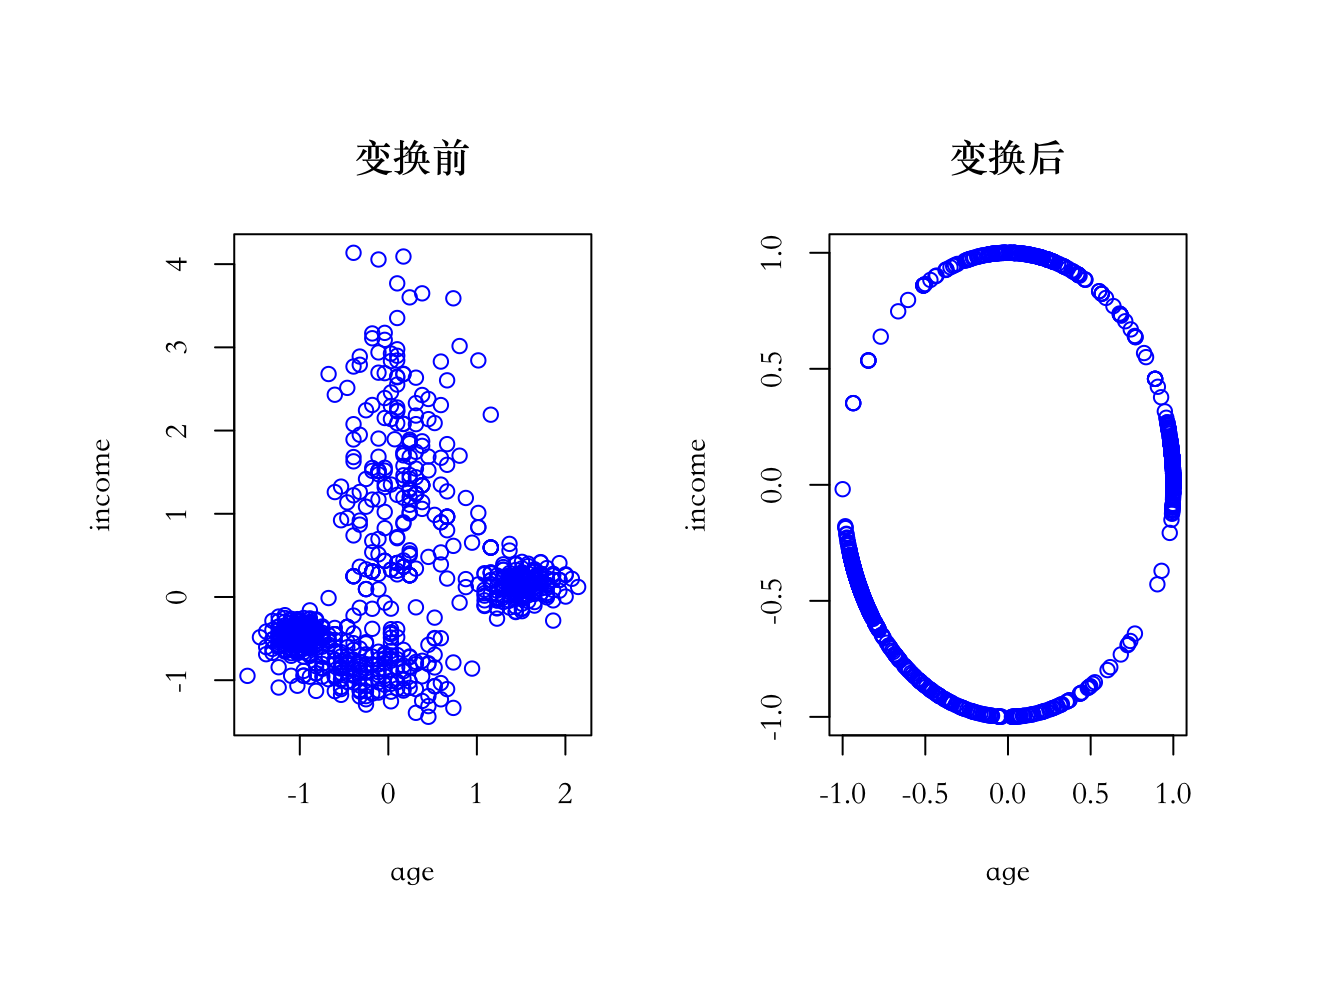
\includegraphics[width=0.8\linewidth]{IDS_files/figure-latex/sst-1} 

}

\caption{Spatial sign transformation}\label{fig:sst}
\end{figure}

Some readers may have found that the above code does not seem to
standardize the data before transformation. Recall the introduction of
KNN, \texttt{preProcess()} with \texttt{method="knnImpute"} by default
will standardize data.

\section{Collinearity}\label{collinearity}

It is probably the technical term known by the most un-technical people.
When two predictors are very strongly correlated, including both in a
model may lead to confusion or problem with a singular matrix. There is
an excellent function in \texttt{corrplot} package with the same name
\texttt{corrplot()} that can visualize correlation structure of a set of
predictors. The function has the option to reorder the variables in a
way that reveals clusters of highly correlated ones.

\begin{Shaded}
\begin{Highlighting}[]
\CommentTok{# select non-survey numerical variables}
\NormalTok{sdat<-}\KeywordTok{subset}\NormalTok{(sim.dat,}\DataTypeTok{select=}\KeywordTok{c}\NormalTok{(}\StringTok{"age"}\NormalTok{,}\StringTok{"income"}\NormalTok{,}\StringTok{"store_exp"}\NormalTok{,}\StringTok{"online_exp"}\NormalTok{,}\StringTok{"store_trans"}\NormalTok{,}\StringTok{"online_trans"} \NormalTok{))}
\CommentTok{# use bagging imputation here}
\NormalTok{imp<-}\KeywordTok{preProcess}\NormalTok{(sdat,}\DataTypeTok{method=}\StringTok{"bagImpute"}\NormalTok{)}
\NormalTok{sdat<-}\KeywordTok{predict}\NormalTok{(imp,sdat)}
\CommentTok{# get the correlation matrix}
\NormalTok{correlation<-}\KeywordTok{cor}\NormalTok{(sdat)}
\CommentTok{# plot }
\KeywordTok{par}\NormalTok{(}\DataTypeTok{oma=}\KeywordTok{c}\NormalTok{(}\DecValTok{2}\NormalTok{,}\DecValTok{2}\NormalTok{,}\DecValTok{2}\NormalTok{,}\DecValTok{2}\NormalTok{))}
\KeywordTok{corrplot.mixed}\NormalTok{(correlation,}\DataTypeTok{order=}\StringTok{"hclust"}\NormalTok{,}\DataTypeTok{tl.pos=}\StringTok{"lt"}\NormalTok{,}\DataTypeTok{upper=}\StringTok{"ellipse"}\NormalTok{)}
\end{Highlighting}
\end{Shaded}

\begin{figure}

{\centering 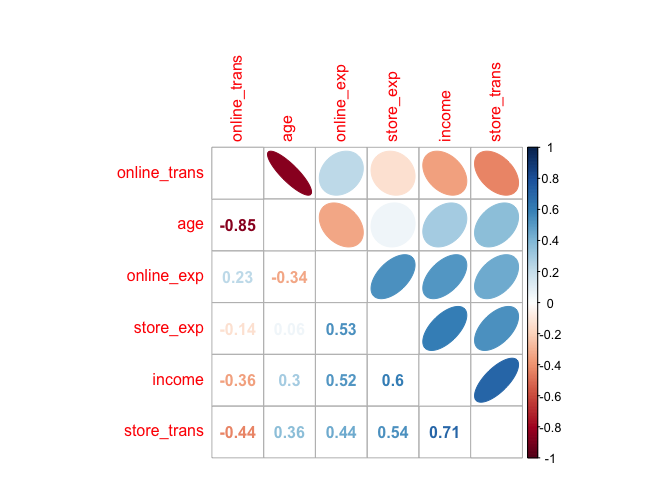
\includegraphics[width=0.8\linewidth]{IDS_files/figure-latex/corp-1} 

}

\caption{Correlation Matrix}\label{fig:corp}
\end{figure}

Here use \texttt{corrplot.mixed()} function to visualize the correlation
matrix (figure \ref{fig:corp}). The closer the correlation is to 0, the
lighter the color is and the closer the shape is to a circle. The
elliptical means the correlation is not equal to 0 (because we set the
\texttt{upper\ =\ "ellipse"}), the greater the correlation, the narrower
the ellipse. Blue represents a positive correlation; red represents a
negative correlation. The direction of the ellipse also changes with the
correlation. The correlation coefficient is shown in the lower triangle
of the matrix. The variables relationship from previous scatter matrix
(figure @ref(fig: scm)) are clear here: the negative correlation between
age and online shopping, the positive correlation between income and
amount of purchasing. Some correlation is very strong ( such as the
correlation between \texttt{online\_trans} and\texttt{age} is -0.85)
which means the two variables contain duplicate information.

Section 3.5 of ``Applied Predictive Modeling'' \citep{APM} presents a
heuristic algorithm to remove a minimum number of predictors to ensure
all pairwise correlations are below a certain threshold:

\begin{quote}
\begin{enumerate}
\def\labelenumi{(\arabic{enumi})}
\tightlist
\item
  Calculate the correlation matrix of the predictors.
\item
  Determine the two predictors associated with the largest absolute
  pairwise correlation (call them predictors A and B).
\item
  Determine the average correlation between A and the other variables.
  Do the same for predictor B.
\item
  If A has a larger average correlation, remove it; otherwise, remove
  predictor B.
\item
  Repeat Step 2-4 until no absolute correlations are above the
  threshold.
\end{enumerate}
\end{quote}

The \texttt{findCorrelation()} function in package \texttt{caret} will
apply the above algorithm.

\begin{Shaded}
\begin{Highlighting}[]
\NormalTok{(highCorr<-}\KeywordTok{findCorrelation}\NormalTok{(}\KeywordTok{cor}\NormalTok{(sdat),}\DataTypeTok{cutoff=}\NormalTok{.}\DecValTok{75}\NormalTok{))}
\end{Highlighting}
\end{Shaded}

\begin{verbatim}
## [1] 1
\end{verbatim}

It returns the index of columns need to be deleted. It tells us that we
need to remove the first column to make sure the correlations are all
below 0.75.

\begin{Shaded}
\begin{Highlighting}[]
\CommentTok{# delete highly correlated columns}
\NormalTok{sdat<-sdat[-highCorr]}
\CommentTok{# check the new correlation matrix}
\KeywordTok{cor}\NormalTok{(sdat)}
\end{Highlighting}
\end{Shaded}

\begin{verbatim}
##               income store_exp online_exp store_trans
## income        1.0000    0.6004     0.5199      0.7070
## store_exp     0.6004    1.0000     0.5350      0.5399
## online_exp    0.5199    0.5350     1.0000      0.4421
## store_trans   0.7070    0.5399     0.4421      1.0000
## online_trans -0.3573   -0.1367     0.2256     -0.4368
##              online_trans
## income            -0.3573
## store_exp         -0.1367
## online_exp         0.2256
## store_trans       -0.4368
## online_trans       1.0000
\end{verbatim}

The absolute value of the elements in the correlation matrix after
removal are all below 0.75. How strong does a correlation have to get,
before you should start worrying about multicollinearity? There is no
easy answer to that question. You can treat the threshold as a tuning
parameter and pick one that gives you best prediction accuracy.

\section{Sparse Variables}\label{sparse-variables}

Other than the highly related predictors, predictors with degenerate
distributions can cause the problem too. Removing those variables can
significantly improve some models' performance and stability (such as
linear regression and logistic regression but the tree based model is
impervious to this type of predictors). One extreme example is a
variable with a single value which is called zero-variance variable.
Variables with very low frequency of unique values are near-zero
variance predictors. In general, detecting those variables follows two
rules:

\begin{itemize}
\tightlist
\item
  The fraction of unique values over the sample size
\item
  The ratio of the frequency of the most prevalent value to the
  frequency of the second most prevalent value.
\end{itemize}

\texttt{nearZeroVar()} function in the \texttt{caret} package can filter
near-zero variance predictors according to the above rules. In order to
show the useage of the function, let's arbitaryly add some problematic
variables to the origional data \texttt{sim.dat}:

\begin{Shaded}
\begin{Highlighting}[]
\CommentTok{# make a copy}
\NormalTok{zero_demo<-sim.dat}
\CommentTok{# add two sparse variable}
\CommentTok{# zero1 only has one unique value}
\CommentTok{# zero2 is a vector with the first element 1 and the rest are 0s}
\NormalTok{zero_demo$zero1<-}\KeywordTok{rep}\NormalTok{(}\DecValTok{1}\NormalTok{,}\KeywordTok{nrow}\NormalTok{(zero_demo))}
\NormalTok{zero_demo$zero2<-}\KeywordTok{c}\NormalTok{(}\DecValTok{1}\NormalTok{,}\KeywordTok{rep}\NormalTok{(}\DecValTok{0}\NormalTok{,}\KeywordTok{nrow}\NormalTok{(zero_demo)-}\DecValTok{1}\NormalTok{))}
\end{Highlighting}
\end{Shaded}

The function will return a vector of integers indicating which columns
to remove:

\begin{Shaded}
\begin{Highlighting}[]
\KeywordTok{nearZeroVar}\NormalTok{(zero_demo,}\DataTypeTok{freqCut =} \DecValTok{95}\NormalTok{/}\DecValTok{5}\NormalTok{, }\DataTypeTok{uniqueCut =} \DecValTok{10}\NormalTok{)}
\end{Highlighting}
\end{Shaded}

As expected, it returns the two columns we generated. You can go ahead
to remove them. Note the two arguments in the function
\texttt{freqCut\ =} and \texttt{uniqueCut\ =} are corresponding to the
previous two rules.

\begin{itemize}
\tightlist
\item
  \texttt{freqCut}: the cutoff for the ratio of the most common value to
  the second most common value
\item
  \texttt{uniqueCut}: the cutoff for the percentage of distinct values
  out of the number of total samples
\end{itemize}

\section{Re-encode Dummy Variables}\label{re-encode-dummy-variables}

A dummy variable is a binary variable (0/1) to represent subgroups of
the sample. Sometimes we need to recode categories to smaller bits of
information named ``dummy variables.'' For example, some questionnaires
have five options for each question, A, B, C, D, and E. After you get
the data, you will usually convert the corresponding categorical
variables for each question into five nominal variables, and then use
one of the options as the baseline.

Let's encode \texttt{gender} and \texttt{house} from \texttt{sim.dat} to
dummy variables. There are two ways to implement this. The first is to
use \texttt{class.ind()} from \texttt{nnet} package. However, it only
works on one variable at a time.

\begin{Shaded}
\begin{Highlighting}[]
\NormalTok{dumVar<-nnet::}\KeywordTok{class.ind}\NormalTok{(sim.dat$gender)}
\KeywordTok{head}\NormalTok{(dumVar)}
\end{Highlighting}
\end{Shaded}

\begin{verbatim}
##      Female Male
## [1,]      1    0
## [2,]      1    0
## [3,]      0    1
## [4,]      0    1
## [5,]      0    1
## [6,]      0    1
\end{verbatim}

Since it is redundant to keep both, we need to remove one of them when
modeling. Another more powerful function is \texttt{dummyVars()} from
\texttt{caret}:

\begin{Shaded}
\begin{Highlighting}[]
\NormalTok{dumMod<-}\KeywordTok{dummyVars}\NormalTok{(~gender+house+income,}
                  \DataTypeTok{data=}\NormalTok{sim.dat,}
                  \CommentTok{# use "origional variable name + level" as new name}
                  \DataTypeTok{levelsOnly=}\NormalTok{F)}
\KeywordTok{head}\NormalTok{(}\KeywordTok{predict}\NormalTok{(dumMod,sim.dat))}
\end{Highlighting}
\end{Shaded}

\begin{verbatim}
##   gender.Female gender.Male house.No house.Yes income
## 1             1           0        0         1 120963
## 2             1           0        0         1 122008
## 3             0           1        0         1 114202
## 4             0           1        0         1 113616
## 5             0           1        0         1 124253
## 6             0           1        0         1 107661
\end{verbatim}

\texttt{dummyVars()} can also use formula format. The variable on the
right-hand side can be both categorical and numeric. For a numerical
variable, the function will keep the variable unchanged. The advantage
is that you can apply the function to a data frame without removing
numerical variables. Other than that, the function can create
interaction term:

\begin{Shaded}
\begin{Highlighting}[]
\NormalTok{dumMod<-}\KeywordTok{dummyVars}\NormalTok{(~gender+house+income+income:gender,}
                  \DataTypeTok{data=}\NormalTok{sim.dat,}
                  \DataTypeTok{levelsOnly=}\NormalTok{F)}
\KeywordTok{head}\NormalTok{(}\KeywordTok{predict}\NormalTok{(dumMod,sim.dat))}
\end{Highlighting}
\end{Shaded}

\begin{verbatim}
##   gender.Female gender.Male house.No house.Yes income
## 1             1           0        0         1 120963
## 2             1           0        0         1 122008
## 3             0           1        0         1 114202
## 4             0           1        0         1 113616
## 5             0           1        0         1 124253
## 6             0           1        0         1 107661
##   gender.Female:income gender.Male:income
## 1               120963                  0
## 2               122008                  0
## 3                    0             114202
## 4                    0             113616
## 5                    0             124253
## 6                    0             107661
\end{verbatim}

If you think the impact income levels on purchasing behavior is
different for male and female, then you may add the interaction term
between \texttt{income} and \texttt{gender}. You can do this by adding
\texttt{income:\ gender} in the formula.

\section{Python Computing}\label{python-computing}

\textbf{Environmental Setup}

\begin{Shaded}
\begin{Highlighting}[]
\ImportTok{from} \NormalTok{IPython.core.interactiveshell }\ImportTok{import} \NormalTok{InteractiveShell}
\NormalTok{InteractiveShell.ast_node_interactivity }\OperatorTok{=} \StringTok{"all"}

\ImportTok{import} \NormalTok{numpy }\ImportTok{as} \NormalTok{np}
\ImportTok{import} \NormalTok{scipy }\ImportTok{as} \NormalTok{sp}
\ImportTok{import} \NormalTok{pandas }\ImportTok{as} \NormalTok{pd}
\ImportTok{import} \NormalTok{math}

\ImportTok{from} \NormalTok{sklearn.preprocessing }\ImportTok{import} \NormalTok{Imputer}
\ImportTok{from} \NormalTok{sklearn.preprocessing }\ImportTok{import} \NormalTok{StandardScaler}

\ImportTok{from} \NormalTok{pandas.plotting }\ImportTok{import} \NormalTok{scatter_matrix}
\ImportTok{import} \NormalTok{matplotlib.pyplot }\ImportTok{as} \NormalTok{plt}
\end{Highlighting}
\end{Shaded}

\subsection{Data Cleaning}\label{data-cleaning-1}

\chapter{Model Tuning Strategy}\label{model-tuning-strategy}

When training a machine learning model, there are many decisions to
make. For example, when training a random forest, you need to decide the
number trees and the number of variables to enter the model. For lasso
method, you need to determine the penalty parameter. There may be
standard settings for some of the parameters, but it's unlikely to guess
the right values for all of these correctly. Other than that, making
good choices on how you split the data into training and testing sets
can make a huge difference in helping you find a high-performance model
efficiently.

This chapter will illustrate the practical aspects of model tuning. We
will talk about different types of model error, sources of model error,
hyperparameter tuning, how to set up your data and how to make sure your
model implementation is correct. In practice applying machine learning
is a highly iterative process.

\section{Systematic Error and Random
Error}\label{systematic-error-and-random-error}

Assume \(\mathbf{X}\) is \(n \times p\) observation matrix and
\(\mathbf{y}\) is response variable, we have:

\[\mathbf{y}=f(\mathbf{X})+\mathbf{\epsilon}\]

where \(\mathbf{\epsilon}\) is the random error with a mean of zero. The
function \(f(\cdot)\) is our modeling target, which represents the
information in the response variable that predictors can explain. The
main goal of estimating \(f(\cdot)\) is inference or prediction, or
sometimes both. In general, there is a trade-off between flexibility and
interpretability of the model. So data scientists need to comprehend the
delicate balance between the two.

Depending on the modeling purposes, the requirement for interpretability
varies. If the prediction is the only goal, then as long as the
prediction is accurate enough, the interpretability is not under
consideration. In this case, people often use ``black box'' model, such
as random forest, boosting tree, neural network and so on. These models
are very flexible but nearly impossible to explain. Their predictive
accuracy is usually higher on the training set, but not necessary when
it predicts. It is not surprising since those models have a huge number
of parameters and high flexibility that they can memorize the entire
training data. A paper by Chiyuan Zhang et al. in 2017 pointed out that
``Deep neural networks (even just two-layer net) easily fit random
labels'' \citep{rethinkDL}. The traditional forms of regularization,
such as weight decay, dropout, and data augmentation, fail to control
generalization error. It poses a conceptual challenge to statistical
theory and also calls our attention when we use such black-box models.

There are two kinds of application problems: complete information
problem and incomplete information problem. The complete information
problem has all the information you need to know the correct response.
Take the famous cat recognition, for example, all the information you
need to identify a cat is in the picture. In this situation, the
algorithm that penetrates the data the most wins. There are some other
similar problems such as the self-driving car, chess game, facial
recognition and speech recognition. But in most of the data science
applications, the information is incomplete. If you want to know whether
a customer is going to purchase again or not, it is unlikely to have
360-degree of the customer's information. You may have their historical
purchasing record, discounts and service received. But you don't know if
the customer sees your ad, or has a friend recommends competitor's
product, or encounters some unhappy purchasing experience somewhere.
There could be a myriad of factors that will influence the customer's
purchase decision while what you have as data is only a small part. To
make things worse, in many cases, you don't even know what you don't
know. Deep learning doesn't have any advantage in solving those
problems. Instead, some parametric models often work better in this
situation. You will comprehend this more after learning the different
types of model error.

Assume we have \(\hat{f}\) which is an estimator of \(f\). Then we can
further get \(\mathbf{\hat{y}}=\hat(f)(\mathbf(X))\). The predicted
error is divided into two parts, systematic error, and random error:

\[E(\mathbf{y}-\hat{\mathbf{y}})^{2}=E[f(\mathbf{X})+\mathbf{\epsilon}-\hat{f}(\mathbf{X})]^{2}=\underset{\text{(1)}}{\underbrace{E[f(\mathbf{X})-\hat{f}(\mathbf{X})]^{2}}}+\underset{\text{(2)}}{\underbrace{Var(\mathbf{\epsilon})}}
\label{eq:error}\]

In the above equation, (1) is the systematic error. It exists because
\(\hat{f}\) usually does not entirely describe the ``systematic
relation'' between X and y which refers to the stable relationship that
exists across different samples. Using a better model can reduce this
kind of the error; (2) is the random error which represents the part of
y that cannot be explained by X. A more complex model does not reduce
the error. The biggest problem with the black-box model is that it fits
random error, i.e., over-fitting. The notable feature of random error is
that it varies over different samples. So one way to determine whether
overfitting happens is to reserve a part of the data as the test set and
then check the performance of the trained model on the test data. Note
that overfitting is a general problem from which any model could suffer.
However, since black-box models usually have a large number of
parameters, it is much more suspectable to over-fitting.

\begin{figure}[htbp]
\centering
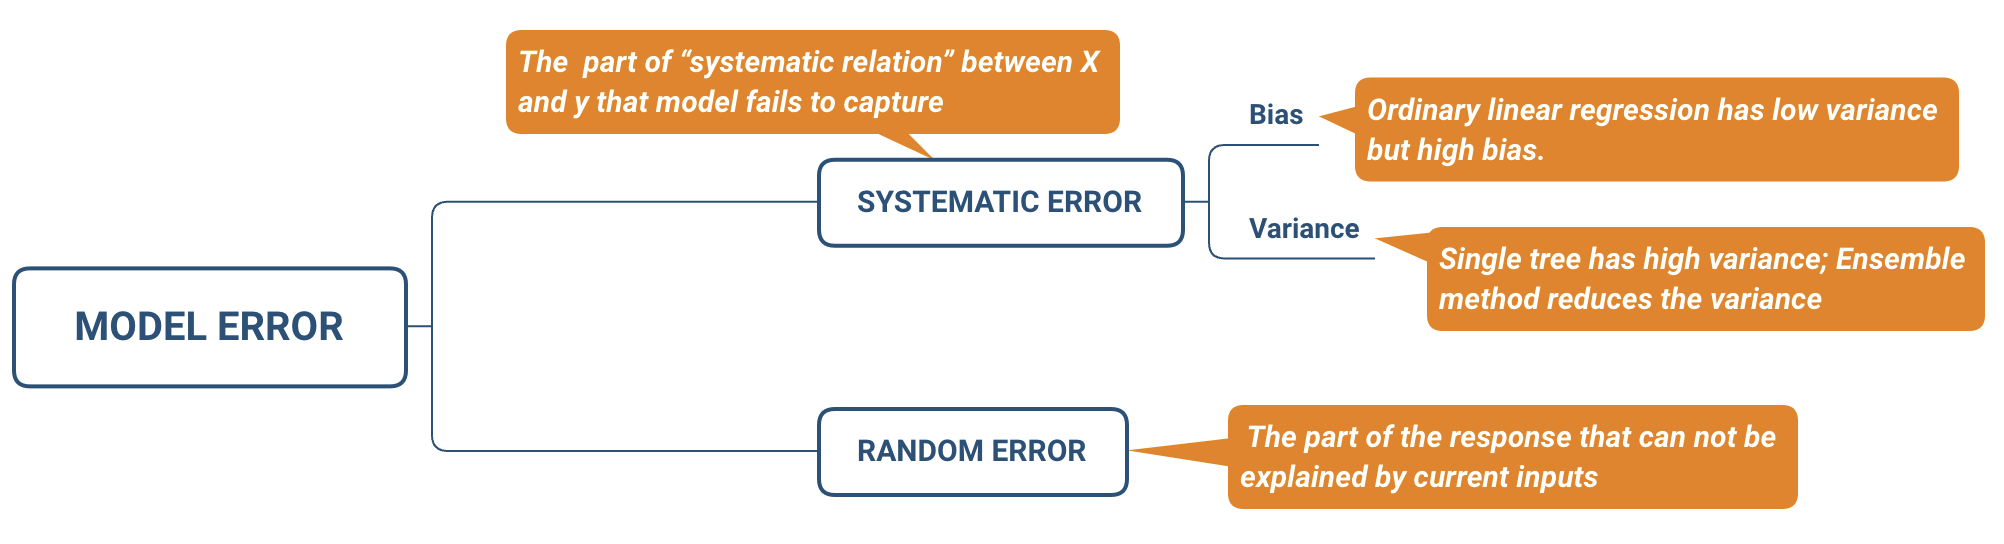
\includegraphics{images/ModelError.png}
\caption{Types of Model Error}
\end{figure}

The systematic error can be further decomposed as:

\[
\begin{array}{ccc}
E[f(\mathbf{X})-\hat{f}(\mathbf{X})]^{2} & = & E\left(f(\mathbf{X})-E[\hat{f}(\mathbf{X})]+E[\hat{f}(\mathbf{X})]-\hat{f}(\mathbf{X})\right)^{2}\\
 & = & E\left(E[\hat{f}(\mathbf{X})]-f(\mathbf{X})\right)^{2}+E\left(\hat{f}(\mathbf{X})-E[\hat{f}(\mathbf{X})]\right)^{2}\\
 & = & [Bias(\hat{f}(\mathbf{X}))]^{2}+Var(\hat{f}(\mathbf{X}))
\end{array}
\]

The systematic error consists of two parts,
\(Bias(\hat{f}(\mathbf{X}))\) and \(Var (\hat{f}(\mathbf{X}))\). To
minimize the systematic error, we need to minimize both. The bias
represents the error caused by the model's approximation of the reality,
i.e., systematic relation, which may be very complex. For example,
linear regression assumes a linear relationship between the predictors
and the response, but rarely is there a perfect linear relationship in
real life. So linear regression is more likely to have a high bias.

To explore bias and variance, let's begin with a simple simulation. We
will simulate a data with a non-linear relationship and fit different
models on it.

The relationship between \(x\) and \(f(x)\) in the following figure is
non-linear. Therefore, despite a large sample size, linear regression
can not give the accurate prediction. In other words, in this case, the
prediction of the linear regression model has a high bias.

\begin{Shaded}
\begin{Highlighting}[]
\KeywordTok{library}\NormalTok{(grid)}
\KeywordTok{library}\NormalTok{(lattice)}
\KeywordTok{library}\NormalTok{(ggplot2)}
\KeywordTok{source}\NormalTok{(}\StringTok{"https://raw.githubusercontent.com/happyrabbit/DataScientistR/master/R/multiplot.r"}\NormalTok{)}
\CommentTok{# randomly simulate some non-linear samples}
\NormalTok{x=}\KeywordTok{seq}\NormalTok{(}\DecValTok{1}\NormalTok{,}\DecValTok{10}\NormalTok{,}\FloatTok{0.01}\NormalTok{)*pi}
\NormalTok{e=}\KeywordTok{rnorm}\NormalTok{(}\KeywordTok{length}\NormalTok{(x),}\DataTypeTok{mean=}\DecValTok{0}\NormalTok{,}\DataTypeTok{sd=}\FloatTok{0.2}\NormalTok{)}
\NormalTok{fx<-}\KeywordTok{sin}\NormalTok{(x)+e+}\KeywordTok{sqrt}\NormalTok{(x)}
\NormalTok{dat=}\KeywordTok{data.frame}\NormalTok{(x,fx)}
\CommentTok{# plot fitting result}
\KeywordTok{ggplot}\NormalTok{(dat,}\KeywordTok{aes}\NormalTok{(x,fx))+}\StringTok{ }
\StringTok{  }\KeywordTok{geom_point}\NormalTok{() +}
\StringTok{  }\KeywordTok{geom_smooth}\NormalTok{(}\DataTypeTok{method =} \StringTok{"lm"}\NormalTok{, }\DataTypeTok{se =} \OtherTok{FALSE}\NormalTok{)}
\end{Highlighting}
\end{Shaded}

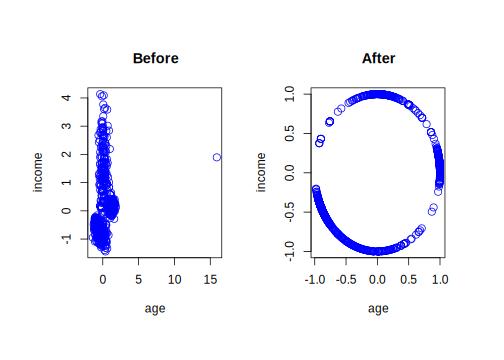
\includegraphics{IDS_files/figure-latex/unnamed-chunk-31-1.pdf}

The estimated parameters will be different for the different training
data. Intuitively, the estimated variance indicates that if we fit the
same model with different data sets, how much the estimated results will
change. Ideally, the change is small. For high variance models, small
changes in the training data result in very different estimates. In
general, a model with high flexibility also has high variance., such as
the CART tree, and the initial boosting method. The Random Forest and
Gradient Boosting Model aim to reduce the variance by summarizing the
results obtained on different samples.

The blue curve in the figure below is obtained by fitting the above
nonlinear observations by a smoothing method, which is highly flexible
and can fit the current data tightly:

\begin{Shaded}
\begin{Highlighting}[]
\KeywordTok{ggplot}\NormalTok{(dat,}\KeywordTok{aes}\NormalTok{(x,fx))+}\KeywordTok{geom_smooth}\NormalTok{(}\DataTypeTok{span =} \FloatTok{0.03}\NormalTok{)}
\end{Highlighting}
\end{Shaded}

\begin{verbatim}
## `geom_smooth()` using method = 'loess' and formula 'y ~ x'
\end{verbatim}

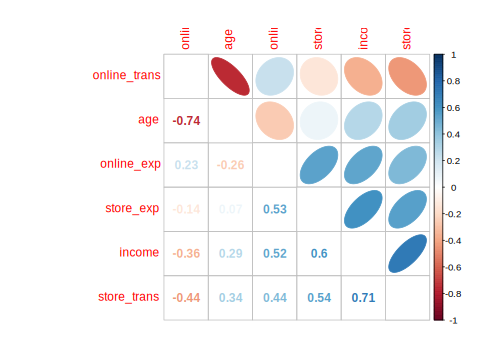
\includegraphics{IDS_files/figure-latex/unnamed-chunk-32-1.pdf}

However, this method has a high variance, and if we simulate different
subsets of the sample, the result curve will change significantly:

\begin{Shaded}
\begin{Highlighting}[]
\CommentTok{# set random seed}
\KeywordTok{set.seed}\NormalTok{(}\DecValTok{2016}\NormalTok{)}
\CommentTok{# sample part of the data to fit model}
\CommentTok{# sample 1}
\NormalTok{idx1=}\KeywordTok{sample}\NormalTok{(}\DecValTok{1}\NormalTok{:}\KeywordTok{length}\NormalTok{(x),}\DecValTok{100}\NormalTok{)}
\NormalTok{dat1=}\KeywordTok{data.frame}\NormalTok{(}\DataTypeTok{x1=}\NormalTok{x[idx1],}\DataTypeTok{fx1=}\NormalTok{fx[idx1])}
\NormalTok{p1=}\KeywordTok{ggplot}\NormalTok{(dat1,}\KeywordTok{aes}\NormalTok{(x1,fx1))+}\KeywordTok{geom_smooth}\NormalTok{(}\DataTypeTok{span =} \FloatTok{0.03}\NormalTok{)}
\CommentTok{# sample 2}
\NormalTok{idx2=}\KeywordTok{sample}\NormalTok{(}\DecValTok{1}\NormalTok{:}\KeywordTok{length}\NormalTok{(x),}\DecValTok{100}\NormalTok{)}
\NormalTok{dat2=}\KeywordTok{data.frame}\NormalTok{(}\DataTypeTok{x2=}\NormalTok{x[idx2],}\DataTypeTok{fx2=}\NormalTok{fx[idx2])}
\NormalTok{p2=}\KeywordTok{ggplot}\NormalTok{(dat2,}\KeywordTok{aes}\NormalTok{(x2,fx2))+}\KeywordTok{geom_smooth}\NormalTok{(}\DataTypeTok{span =} \FloatTok{0.03}\NormalTok{)}
\CommentTok{# sample 3}
\NormalTok{idx3=}\KeywordTok{sample}\NormalTok{(}\DecValTok{1}\NormalTok{:}\KeywordTok{length}\NormalTok{(x),}\DecValTok{100}\NormalTok{)}
\NormalTok{dat3=}\KeywordTok{data.frame}\NormalTok{(}\DataTypeTok{x3=}\NormalTok{x[idx3],}\DataTypeTok{fx3=}\NormalTok{fx[idx3])}
\NormalTok{p3=}\KeywordTok{ggplot}\NormalTok{(dat3,}\KeywordTok{aes}\NormalTok{(x3,fx3))+}\KeywordTok{geom_smooth}\NormalTok{(}\DataTypeTok{span =} \FloatTok{0.03}\NormalTok{)}
\CommentTok{# sample 4}
\NormalTok{idx4=}\KeywordTok{sample}\NormalTok{(}\DecValTok{1}\NormalTok{:}\KeywordTok{length}\NormalTok{(x),}\DecValTok{100}\NormalTok{)}
\NormalTok{dat4=}\KeywordTok{data.frame}\NormalTok{(}\DataTypeTok{x4=}\NormalTok{x[idx4],}\DataTypeTok{fx4=}\NormalTok{fx[idx4])}
\NormalTok{p4=}\KeywordTok{ggplot}\NormalTok{(dat4,}\KeywordTok{aes}\NormalTok{(x4,fx4))+}\KeywordTok{geom_smooth}\NormalTok{(}\DataTypeTok{span =} \FloatTok{0.03}\NormalTok{)}
\KeywordTok{multiplot}\NormalTok{(p1,p2,p3,p4,}\DataTypeTok{cols=}\DecValTok{2}\NormalTok{)}
\end{Highlighting}
\end{Shaded}

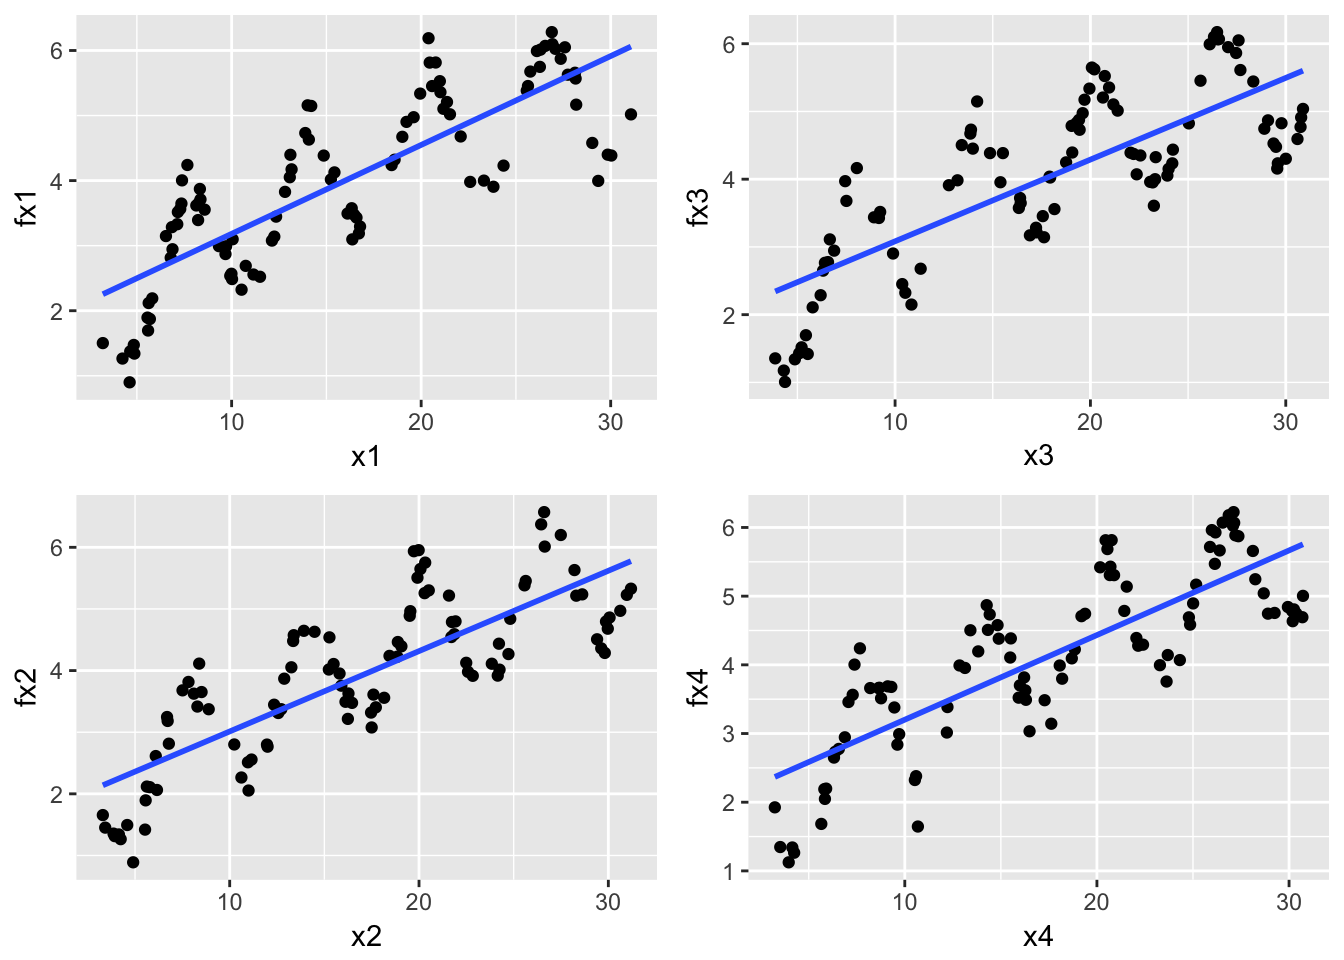
\includegraphics{IDS_files/figure-latex/unnamed-chunk-33-1.pdf}

Fitting the linear model using the same four subsets, the result barely
changes:

\begin{Shaded}
\begin{Highlighting}[]
\NormalTok{p1=}\KeywordTok{ggplot}\NormalTok{(dat1,}\KeywordTok{aes}\NormalTok{(x1,fx1))+}\StringTok{ }
\StringTok{  }\KeywordTok{geom_point}\NormalTok{() +}
\StringTok{  }\KeywordTok{geom_smooth}\NormalTok{(}\DataTypeTok{method =} \StringTok{"lm"}\NormalTok{, }\DataTypeTok{se =} \OtherTok{FALSE}\NormalTok{)}
\NormalTok{p2=}\KeywordTok{ggplot}\NormalTok{(dat2,}\KeywordTok{aes}\NormalTok{(x2,fx2))+}\StringTok{ }
\StringTok{  }\KeywordTok{geom_point}\NormalTok{() +}
\StringTok{  }\KeywordTok{geom_smooth}\NormalTok{(}\DataTypeTok{method =} \StringTok{"lm"}\NormalTok{, }\DataTypeTok{se =} \OtherTok{FALSE}\NormalTok{)}
\NormalTok{p3=}\KeywordTok{ggplot}\NormalTok{(dat3,}\KeywordTok{aes}\NormalTok{(x3,fx3))+}\StringTok{ }
\StringTok{  }\KeywordTok{geom_point}\NormalTok{() +}
\StringTok{  }\KeywordTok{geom_smooth}\NormalTok{(}\DataTypeTok{method =} \StringTok{"lm"}\NormalTok{, }\DataTypeTok{se =} \OtherTok{FALSE}\NormalTok{)}
\NormalTok{p4=}\KeywordTok{ggplot}\NormalTok{(dat4,}\KeywordTok{aes}\NormalTok{(x4,fx4))+}\StringTok{ }
\StringTok{  }\KeywordTok{geom_point}\NormalTok{() +}
\StringTok{  }\KeywordTok{geom_smooth}\NormalTok{(}\DataTypeTok{method =} \StringTok{"lm"}\NormalTok{, }\DataTypeTok{se =} \OtherTok{FALSE}\NormalTok{)}
\KeywordTok{multiplot}\NormalTok{(p1,p2,p3,p4,}\DataTypeTok{cols=}\DecValTok{2}\NormalTok{)}
\end{Highlighting}
\end{Shaded}

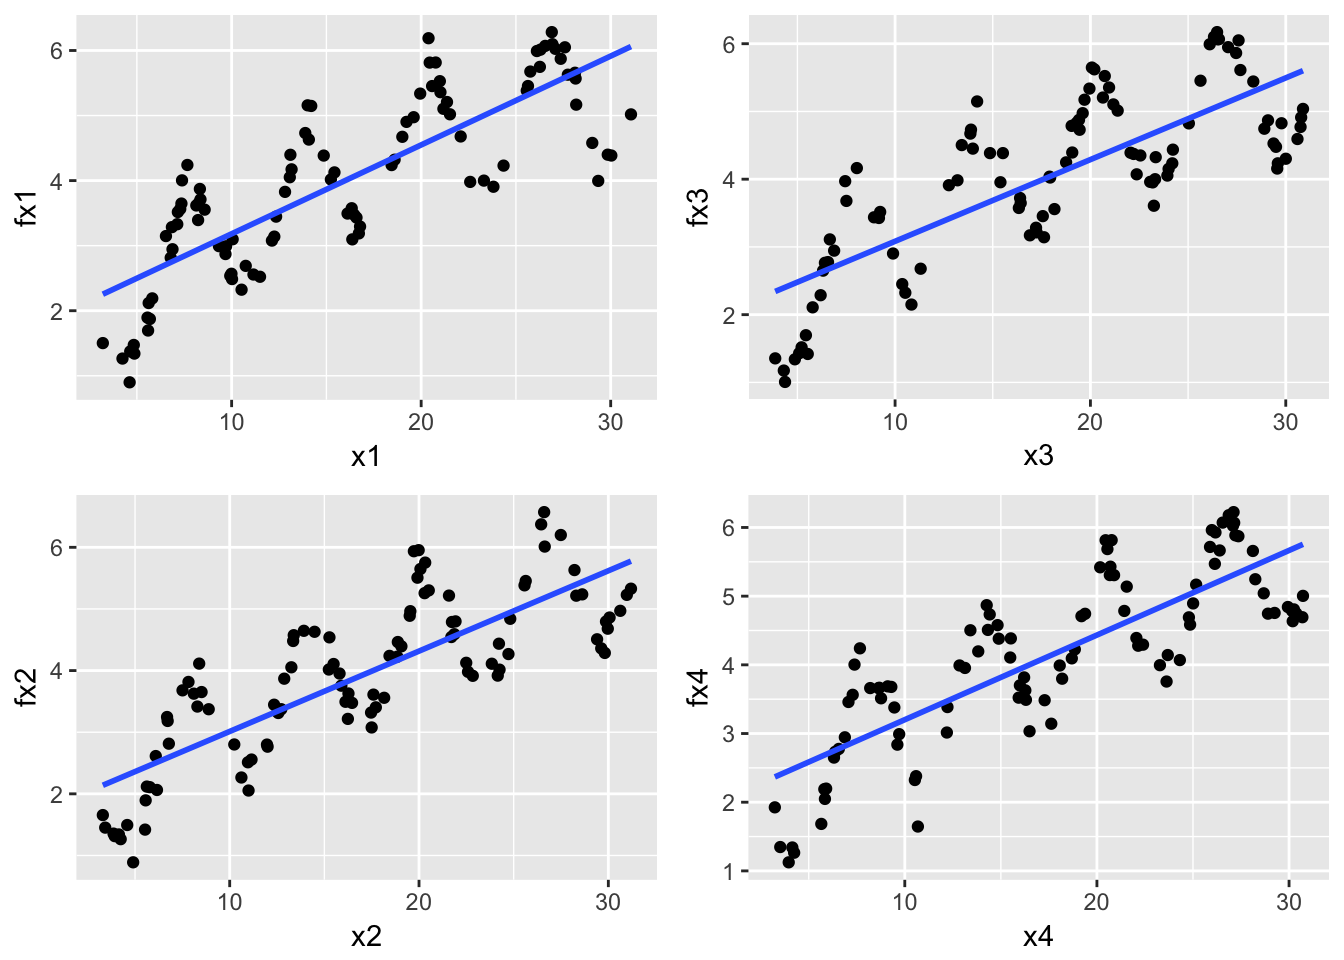
\includegraphics{IDS_files/figure-latex/unnamed-chunk-34-1.pdf}

In general, the variance (\(Var(\hat{f}(\mathbf{X}))\))
\textbf{increases} and the bias (\(Bias(\hat{f}(\mathbf{X}))\))
\textbf{decreases} as the model flexibility increases. Variance and bias
together determine the systematic error (or mean square error, MSE). As
we increase the flexibility of the model, at first the rate at which
\(Bias(\hat{f}(\mathbf{X}))\) decreases is faster than
\(Var (\hat{f} (\mathbf{X}))\), so the MSE decreases. However, to some
degree, higher flexibility has little effect on
\(Bias(\hat{f}(\mathbf{X}))\) but \(Var(\hat{f} (\mathbf{X}))\)
increases significantly, so the MSE increases.

\subsection{Measurement Error in the
Response}\label{measurement-error-in-the-response}

The random error (\(\mathbf{\epsilon}\)) reflects the measurement error
in the response. This part of the error is irreducible, and so it makes
the root mean square error (RMSE) and \(R^2\) have the corresponding
upper and lower limits. RMSE and \(R^2\) are commonly used performance
measures for the regression model which we will talk in more detail
later. Therefore, the random error term not only represents the part of
fluctuations the model cannot explain but also contains measurement
error in the response variables. Section 20.2 of Applied Predictive
Modeling \citep{APM} has an example that shows the effect of the
measurement error in the response variable on the model performance
(RMSE and \(R^2\)).

The authors increased the error in the response proportional to a base
level error which was gotten using the original data without introducing
extra noise. Then fit a set of models repeatedly using the
``contaminated'' data sets to study the change of \(RMSE\) and \(R^2\)
as the level of noise. Here we use clothing consumer data for a similar
illustration. Suppose many people do not want to disclose their income
and so we need to use other variables to establish a model to predict
income. We set up the following model:

\begin{Shaded}
\begin{Highlighting}[]
\CommentTok{# load data}
\NormalTok{sim.dat <-}\StringTok{ }\KeywordTok{read.csv}\NormalTok{(}\StringTok{"https://raw.githubusercontent.com/happyrabbit/DataScientistR/master/Data/SegData.csv "}\NormalTok{)}
\NormalTok{ymad<-}\KeywordTok{mad}\NormalTok{(}\KeywordTok{na.omit}\NormalTok{(sim.dat$income))}
\CommentTok{# calculate z-score}
\NormalTok{zs<-(sim.dat$income-}\KeywordTok{mean}\NormalTok{(}\KeywordTok{na.omit}\NormalTok{(sim.dat$income)))/ymad}
\CommentTok{# which(na.omit(zs>3.5)): identify outliers}
\CommentTok{# which(is.na(zs)): identify missing values}
\NormalTok{idex<-}\KeywordTok{c}\NormalTok{(}\KeywordTok{which}\NormalTok{(}\KeywordTok{na.omit}\NormalTok{(zs>}\FloatTok{3.5}\NormalTok{)),}\KeywordTok{which}\NormalTok{(}\KeywordTok{is.na}\NormalTok{(zs)))}
\CommentTok{# delete rows with outliers and missing values}
\NormalTok{sim.dat<-sim.dat[-idex,]}
\NormalTok{fit<-}\KeywordTok{lm}\NormalTok{(income~store_exp+online_exp+store_trans+online_trans,}\DataTypeTok{data=}\NormalTok{sim.dat)}
\end{Highlighting}
\end{Shaded}

The output shows that without additional noise, the root mean square
error (RMSE) of the model is 29567, \(R^2\) is 0.6.

Let's add various degrees of noise (0 to 3 times the RMSE) to the
variable \texttt{income}:

\[ RMSE \times (0.0, 0.5, 1.0, 1.5, 2.0, 2.5, 3.0) \]

\begin{Shaded}
\begin{Highlighting}[]
\NormalTok{noise<-}\KeywordTok{matrix}\NormalTok{(}\KeywordTok{rep}\NormalTok{(}\OtherTok{NA}\NormalTok{,}\DecValTok{7}\NormalTok{*}\KeywordTok{nrow}\NormalTok{(sim.dat)),}\DataTypeTok{nrow=}\KeywordTok{nrow}\NormalTok{(sim.dat),}\DataTypeTok{ncol=}\DecValTok{7}\NormalTok{)}
\NormalTok{for (i in }\DecValTok{1}\NormalTok{:}\KeywordTok{nrow}\NormalTok{(sim.dat))\{}
\NormalTok{noise[i,]<-}\KeywordTok{rnorm}\NormalTok{(}\DecValTok{7}\NormalTok{,}\KeywordTok{rep}\NormalTok{(}\DecValTok{0}\NormalTok{,}\DecValTok{7}\NormalTok{),}\KeywordTok{summary}\NormalTok{(fit)$sigma*}\KeywordTok{seq}\NormalTok{(}\DecValTok{0}\NormalTok{,}\DecValTok{3}\NormalTok{,}\DataTypeTok{by=}\FloatTok{0.5}\NormalTok{))}
\NormalTok{\}}
\end{Highlighting}
\end{Shaded}

We then examine the effect of noise intensity on \(R^2\) for models with
different complexity. The models with complexity from low to high are:
ordinary linear regression, partial least square regression(PLS),
multivariate adaptive regression spline (MARS), support vector machine
(SVM, the kernel function is radial basis function), and random forest.

\begin{Shaded}
\begin{Highlighting}[]
\CommentTok{# fit ordinary linear regression}
\NormalTok{rsq_linear<-}\KeywordTok{rep}\NormalTok{(}\DecValTok{0}\NormalTok{,}\KeywordTok{ncol}\NormalTok{(noise))}
\NormalTok{for (i in }\DecValTok{1}\NormalTok{:}\DecValTok{7}\NormalTok{)\{}
\NormalTok{withnoise<-sim.dat$income+noise[,i]}
\NormalTok{fit0<-}\KeywordTok{lm}\NormalTok{(withnoise~store_exp+online_exp+store_trans+online_trans,}\DataTypeTok{data=}\NormalTok{sim.dat)}
\NormalTok{rsq_linear[i]<-}\KeywordTok{summary}\NormalTok{(fit0)$adj.r.squared}
\NormalTok{\}}
\end{Highlighting}
\end{Shaded}

PLS is a method of linearizing nonlinear relationships through hidden
layers. It is similar to the principal component regression (PCR),
except that PCR does not take into account the information of the
dependent variable when selecting the components, and its purpose is to
find the linear combinations (i.e., unsupervised) that capture the most
variance of the independent variables. When the independent variables
and response variables are related, PCR can well identify the systematic
relationship between them. However, when there exist independent
variables not associated with response variable, it will undermine PCR's
performance. And PLS maximizes the linear combination of dependencies
with the response variable. In the current case, the more complicated
PLS does not perform better than simple linear regression.

\begin{Shaded}
\begin{Highlighting}[]
\CommentTok{# pls: conduct PLS and PCR}
\KeywordTok{library}\NormalTok{(pls)}
\NormalTok{rsq_pls<-}\KeywordTok{rep}\NormalTok{(}\DecValTok{0}\NormalTok{,}\KeywordTok{ncol}\NormalTok{(noise))}
\CommentTok{# fit PLS}
\NormalTok{for (i in }\DecValTok{1}\NormalTok{:}\DecValTok{7}\NormalTok{)\{}
\NormalTok{withnoise<-sim.dat$income+noise[,i]}
\NormalTok{fit0<-}\KeywordTok{plsr}\NormalTok{(withnoise~store_exp+online_exp+store_trans+online_trans,}\DataTypeTok{data=}\NormalTok{sim.dat)}
\NormalTok{rsq_pls[i]<-}\KeywordTok{max}\NormalTok{(}\KeywordTok{drop}\NormalTok{(}\KeywordTok{R2}\NormalTok{(fit0, }\DataTypeTok{estimate =} \StringTok{"train"}\NormalTok{,}\DataTypeTok{intercept =} \OtherTok{FALSE}\NormalTok{)$val))}
\NormalTok{\}}
\end{Highlighting}
\end{Shaded}

\begin{Shaded}
\begin{Highlighting}[]
\CommentTok{# earth: fit mars }
\KeywordTok{library}\NormalTok{(earth)}
\NormalTok{rsq_mars<-}\KeywordTok{rep}\NormalTok{(}\DecValTok{0}\NormalTok{,}\KeywordTok{ncol}\NormalTok{(noise))}
\NormalTok{for (i in }\DecValTok{1}\NormalTok{:}\DecValTok{7}\NormalTok{)\{}
\NormalTok{withnoise<-sim.dat$income+noise[,i]}
\NormalTok{fit0<-}\KeywordTok{earth}\NormalTok{(withnoise~store_exp+online_exp+store_trans+online_trans,}\DataTypeTok{data=}\NormalTok{sim.dat)}
\NormalTok{rsq_mars[i]<-fit0$rsq}
\NormalTok{\}}
\end{Highlighting}
\end{Shaded}

\begin{Shaded}
\begin{Highlighting}[]
\CommentTok{# caret: awesome package for tuning predictive model}
\KeywordTok{library}\NormalTok{(caret)}
\NormalTok{rsq_svm<-}\KeywordTok{rep}\NormalTok{(}\DecValTok{0}\NormalTok{,}\KeywordTok{ncol}\NormalTok{(noise))}
\CommentTok{# Need some time to run}
\NormalTok{for (i in }\DecValTok{1}\NormalTok{:}\DecValTok{7}\NormalTok{)\{}
\NormalTok{idex<-}\KeywordTok{which}\NormalTok{(}\KeywordTok{is.na}\NormalTok{(sim.dat$income))}
\NormalTok{withnoise<-sim.dat$income+noise[,i]}
\NormalTok{trainX<-sim.dat[,}\KeywordTok{c}\NormalTok{(}\StringTok{"store_exp"}\NormalTok{,}\StringTok{"online_exp"}\NormalTok{,}\StringTok{"store_trans"}\NormalTok{,}\StringTok{"online_trans"}\NormalTok{)]}
\NormalTok{trainY<-withnoise}
\NormalTok{fit0<-}\KeywordTok{train}\NormalTok{(trainX,trainY,}\DataTypeTok{method=}\StringTok{"svmRadial"}\NormalTok{,}
            \DataTypeTok{tuneLength=}\DecValTok{15}\NormalTok{,}
            \DataTypeTok{trControl=}\KeywordTok{trainControl}\NormalTok{(}\DataTypeTok{method=}\StringTok{"cv"}\NormalTok{))}
\NormalTok{rsq_svm[i]<-}\KeywordTok{max}\NormalTok{(fit0$results$Rsquared)}
\NormalTok{\}}
\end{Highlighting}
\end{Shaded}

\begin{Shaded}
\begin{Highlighting}[]
\CommentTok{# randomForest: random forest model}
\KeywordTok{library}\NormalTok{(randomForest)}
\NormalTok{rsq_rf<-}\KeywordTok{rep}\NormalTok{(}\DecValTok{0}\NormalTok{,}\KeywordTok{ncol}\NormalTok{(noise))}
\CommentTok{# ntree=500 number of trees}
\CommentTok{# na.action = na.omit  ignore missing value}
\NormalTok{for (i in }\DecValTok{1}\NormalTok{:}\DecValTok{7}\NormalTok{)\{}
\NormalTok{withnoise<-sim.dat$income+noise[,i]}
\NormalTok{fit0<-}\KeywordTok{randomForest}\NormalTok{(withnoise~store_exp+online_exp+store_trans+online_trans,}\DataTypeTok{data=}\NormalTok{sim.dat,}\DataTypeTok{ntree=}\DecValTok{500}\NormalTok{,}\DataTypeTok{na.action =} \NormalTok{na.omit)}
\NormalTok{rsq_rf[i]<-}\KeywordTok{tail}\NormalTok{(fit0$rsq,}\DecValTok{1}\NormalTok{)}
\NormalTok{\}}
\KeywordTok{library}\NormalTok{(reshape2)}
\NormalTok{rsq<-}\KeywordTok{data.frame}\NormalTok{(}\KeywordTok{cbind}\NormalTok{(}\DataTypeTok{Noise=}\KeywordTok{c}\NormalTok{(}\FloatTok{0.0}\NormalTok{, }\FloatTok{0.5}\NormalTok{, }\FloatTok{1.0}\NormalTok{, }\FloatTok{1.5}\NormalTok{, }\FloatTok{2.0}\NormalTok{, }\FloatTok{2.5}\NormalTok{, }\FloatTok{3.0}\NormalTok{),rsq_linear,rsq_pls,rsq_mars,rsq_svm,rsq_rf))}
\NormalTok{rsq<-}\KeywordTok{melt}\NormalTok{(rsq,}\DataTypeTok{id.vars=}\StringTok{"Noise"}\NormalTok{,}\DataTypeTok{measure.vars=}\KeywordTok{c}\NormalTok{(}\StringTok{"rsq_linear"}\NormalTok{,}\StringTok{"rsq_pls"}\NormalTok{,}\StringTok{"rsq_mars"}\NormalTok{,}\StringTok{"rsq_svm"}\NormalTok{,}\StringTok{"rsq_rf"}\NormalTok{))}
\end{Highlighting}
\end{Shaded}







\begin{Shaded}
\begin{Highlighting}[]
\KeywordTok{library}\NormalTok{(ggplot2)}
\KeywordTok{ggplot}\NormalTok{(}\DataTypeTok{data=}\NormalTok{rsq, }\KeywordTok{aes}\NormalTok{(}\DataTypeTok{x=}\NormalTok{Noise, }\DataTypeTok{y=}\NormalTok{value, }\DataTypeTok{group=}\NormalTok{variable, }\DataTypeTok{colour=}\NormalTok{variable)) +}
\StringTok{    }\KeywordTok{geom_line}\NormalTok{() +}
\StringTok{    }\KeywordTok{geom_point}\NormalTok{()+}
\StringTok{  }\KeywordTok{ylab}\NormalTok{(}\StringTok{"R2"}\NormalTok{) }
\end{Highlighting}
\end{Shaded}

\begin{figure}

{\centering 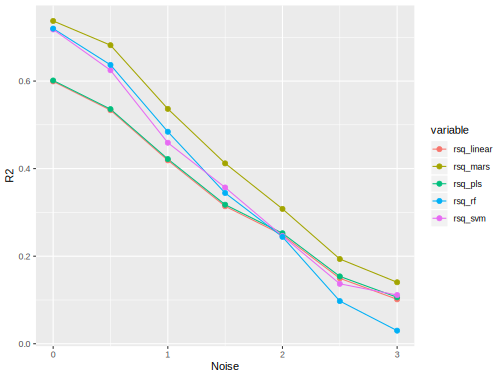
\includegraphics[width=0.8\linewidth]{IDS_files/figure-latex/error-1} 

}

\caption{Test set \(R^2\) profiles for income models when
measurement system noise increases. \texttt{rsq\_linear}: linear
regression, \texttt{rsq\_pls}: Partial Least Square, \texttt{rsq\_mars}:
Multiple Adaptive Regression Spline Regression, \texttt{rsq\_svm}:
Support Vector Machine,\texttt{rsq\_rf}: Random Forest}\label{fig:error}
\end{figure}

Fig. \ref{fig:error} shows that:

All model performance decreases sharply with increasing noise intensity.
To better anticipate model performance, it helps to understand the way
variable is measured. It is something need to make clear at the
beginning of an analytical project. A data scientist should be aware of
the quality of the data in the database. For data from the clients, it
is an important to understand the quality of the data by communication.

More complex model is not necessarily better. The best model in this
situation is MARS, not random forests or SVM. Simple linear regression
and PLS perform the worst when noise is low. MARS is more complicated
than the linear regression and PLS, but it is simpler and easier to
explain than random forest and SVM.

When noise increases to a certain extent, the potential structure
becomes vaguer, and complex random forest model starts to fail. When the
systematic measurement error is significant, a more straightforward but
not naive model may be a better choice. It is always a good practice to
try different models, and select the simplest model in the case of
similar performance. Model evaluation and selection represent the career
``maturity'' of a data scientist.

\subsection{Measurement Error in the Independent
Variables}\label{measurement-error-in-the-independent-variables}

The traditional statistical model usually assumes that the measurement
of the independent variable has no error which is not possible in
practice. Considering the error in the independent variables is
necessary. The impact of the error depends on the following factors: (1)
the magnitude of the randomness; (2) the importance of the corresponding
variable in the model, and (3) the type of model used. Use variable
\texttt{online\_exp} as an example. The approach is similar to the
previous section. Add varying degrees of noise and see its impact on the
model performance. We add the following different levels of noise (0 to
3 times the standard deviation) to\texttt{online\_exp}:

\[\sigma_{0} \times (0.0, 0.5, 1.0, 1.5, 2.0, 2.5, 3.0)\]

where \(\sigma_{0}\) is the standard error of \texttt{online\_exp}.

\begin{Shaded}
\begin{Highlighting}[]
\NormalTok{noise<-}\KeywordTok{matrix}\NormalTok{(}\KeywordTok{rep}\NormalTok{(}\OtherTok{NA}\NormalTok{,}\DecValTok{7}\NormalTok{*}\KeywordTok{nrow}\NormalTok{(sim.dat)),}\DataTypeTok{nrow=}\KeywordTok{nrow}\NormalTok{(sim.dat),}\DataTypeTok{ncol=}\DecValTok{7}\NormalTok{)}
\NormalTok{for (i in }\DecValTok{1}\NormalTok{:}\KeywordTok{nrow}\NormalTok{(sim.dat))\{}
\NormalTok{noise[i,]<-}\KeywordTok{rnorm}\NormalTok{(}\DecValTok{7}\NormalTok{,}\KeywordTok{rep}\NormalTok{(}\DecValTok{0}\NormalTok{,}\DecValTok{7}\NormalTok{),}\KeywordTok{sd}\NormalTok{(sim.dat$online_exp)*}\KeywordTok{seq}\NormalTok{(}\DecValTok{0}\NormalTok{,}\DecValTok{3}\NormalTok{,}\DataTypeTok{by=}\FloatTok{0.5}\NormalTok{))}
\NormalTok{\}}
\end{Highlighting}
\end{Shaded}

Likewise, we examine the effect of noise intensity on different models
(\(R^2\)). The models with complexity from low to high are: ordinary
linear regression, partial least square regression(PLS), multivariate
adaptive regression spline (MARS), support vector machine (SVM, the
Kernel function is radial basis function), and random forest. The code
is similar as before so not shown here.








\begin{figure}

{\centering 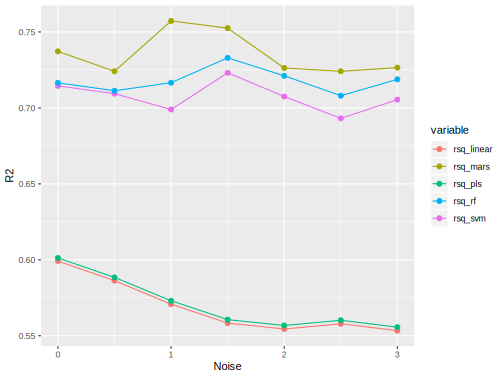
\includegraphics[width=0.8\linewidth]{IDS_files/figure-latex/errorvariable-1} 

}

\caption{Test set \(R^2\) profiles for income models when
noise in \texttt{online\_exp} increases. \texttt{rsq\_linear} : linear
regression, \texttt{rsq\_pls} : Partial Least Square,
\texttt{rsq\_mars}: Multiple Adaptive Regression Spline Regression,
\texttt{rsq\_svm}: Support Vector Machine,\texttt{rsq\_rf}: Random
Forest}\label{fig:errorvariable}
\end{figure}

Comparing Fig. \ref{fig:errorvariable} and Fig. \ref{fig:error}, the
influence of the two types of error is very different. The error in
response cannot be overcome for any model, but it is not the case for
the independent variables. Imagine an extreme case, if
\texttt{online\_exp} is completely random, that is, no information in
it, the impact on the performance of random forest and support vector
machine is marginal. Linear regression and PLS still perform similarly.
With the increase of noise, the performance starts to decline faster. To
a certain extent, it becomes steady. In general, if an independent
variable contains error, other variables associated with it can
compensate to some extent.

\section{Data Splitting and
Resampling}\label{data-splitting-and-resampling}

Those highly adaptable models can model complex relationships. However,
they tend to overfit which leads to the poor prediction by learning too
much from the data. It means that the model is susceptible to the
specific sample used to fit it. When future data is not exactly like the
past data, the model prediction may have big mistakes. A simple model
like ordinary linear regression tends instead to underfit which leads to
a bad prediction by learning too little from the data. It systematically
over-predicts or under-predicts the data regardless of how well future
data resemble past data. Without evaluating models, the modeler will not
know about the problem before the future samples. Data splitting and
resampling are fundamental techniques to build sound models for
prediction.

\emph{Data splitting} is to put part of the data aside as testing set
(or Hold-outs, out of bag samples) and use the rest for model training.
Training samples are also called in-sample. Model performance metrics
evaluated using in-sample are retrodictive, not predictive.

The traditional business intelligence usually handles data description.
Answer simple questions by querying and summarizing the data, such as:

\begin{itemize}
\tightlist
\item
  What is the monthly sales of a product in 2015?
\item
  What is the number of visits to our site in the past month?\\
\item
  What is the sales difference in 2015 for two different product
  designs?
\end{itemize}

There is no need to go through the tedious process of splitting the
data, tuning and testing model to answer questions of this kind.
Instead, people usually use as complete data as possible and then sum or
average the parts of interest.

Many models have parameters which cannot be directly estimated from the
data, such as \(\lambda\) in the lasso (penalty parameter), the number
of trees in the random forest. This type of model parameter is called
tuning parameter, and there is no analytical formula available to
calculate the optimizing value. Tuning parameters often control the
complexity of the model. Poor choice for the values can result in
over-fitting or under-fitting. A standard approach to estimate tuning
parameters is through cross-validation which is a data resampling
approach.

Since to get reasonable precision of the performance values on a single
test set, the size of the test set may need to be large. So more often,
people will instead resample the training set. \emph{Data resampling}
operates similarly: use a subset of samples to fit a model and use the
rest to evaluate model performance. This process will repeat multiple
times to get a performance profile. In that sense, resampling is based
on splitting. The general steps are:

\begin{itemize}
\tightlist
\item
  Define a set of candidate values for tuning parameter(s)

  \begin{itemize}
  \tightlist
  \item
    For each candidate value in the set

    \begin{itemize}
    \tightlist
    \item
      Resample data
    \item
      Fit model
    \item
      Predict hold-out
    \item
      Calculate performance
    \end{itemize}
  \end{itemize}
\item
  Aggregate the results
\item
  Determine the final tuning parameter
\item
  Refit the model with the entire training set
\end{itemize}

\begin{figure}[htbp]
\centering
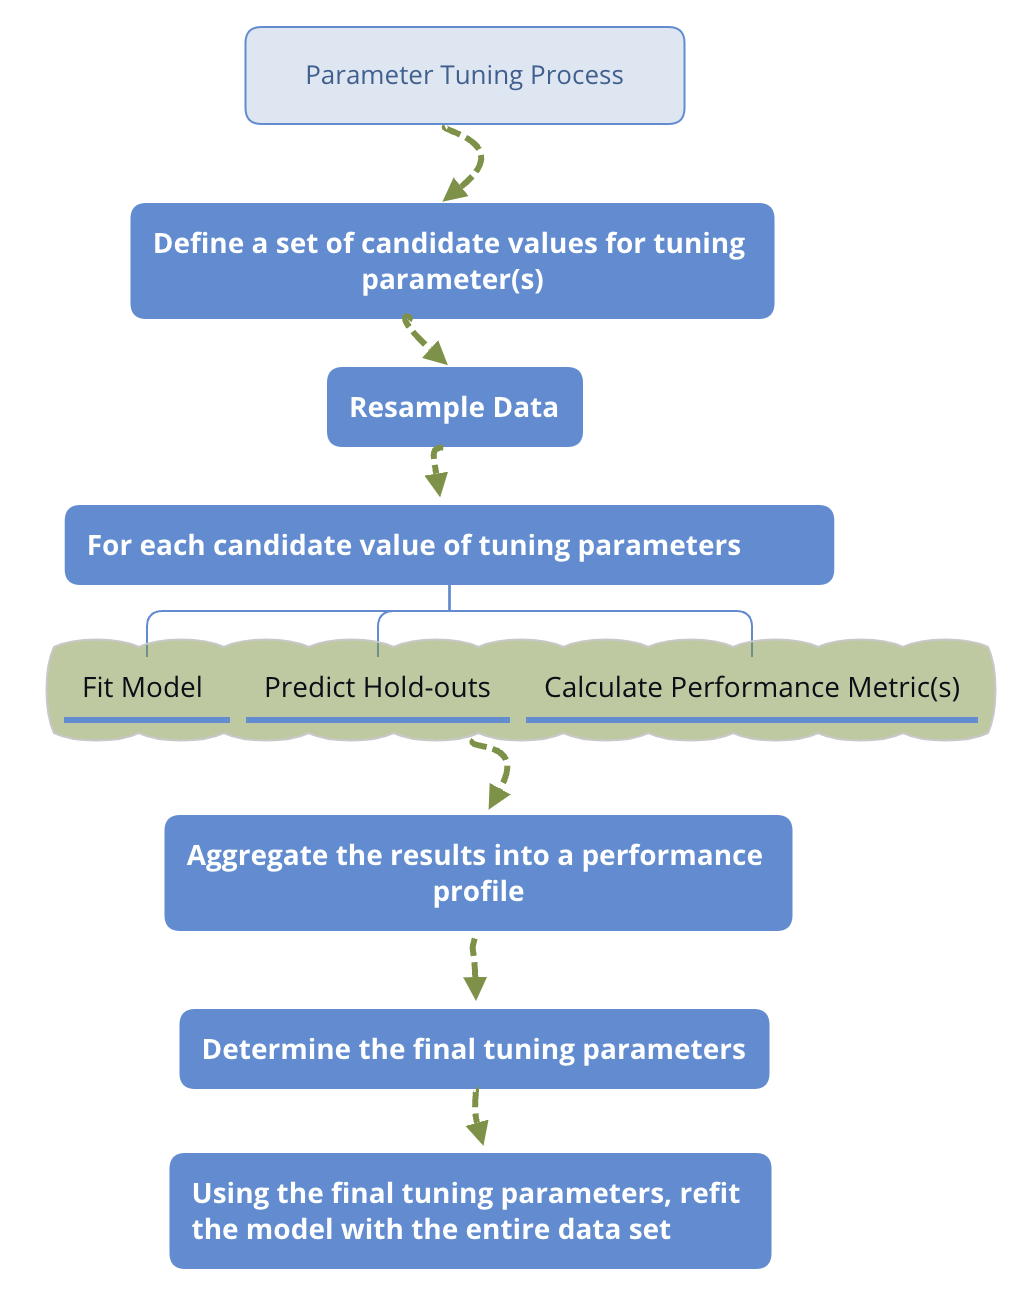
\includegraphics[width=0.80000\textwidth]{images/ParameterTuningProcess.png}
\caption{Parameter Tuning Process}
\end{figure}

We have outlined above the general procedure to tune parameters. Now
let's focus on the critical part of the process: data splitting.

\chapter{References}\label{references}

\bibliography{bibliography.bib}

\backmatter
\printindex

\end{document}
